\documentclass[a4paper, 12pt]{report}

\usepackage[dvipsnames]{xcolor}

%%%%%%%%%%%%%%%%
% Set Variables %
%%%%%%%%%%%%%%%%

\def\useItalian{0}  % 1 = Italian, 0 = English

\def\courseName{Graph Theory}

\def\coursePrerequisites{Sufficient knowledge of algorithm design, probability and combinatorics}

\def\book{\curlyquotes{Graph Theory}, R. Diestel}

\def\authorName{Simone Bianco}
\def\email{bianco.simone@outlook.it}
\def\github{https://github.com/Exyss/university-notes}
\def\linkedin{https://www.linkedin.com/in/simone-bianco}

%%%%%%%%%%%%
% Packages %
%%%%%%%%%%%%

\usepackage{../../packages/Nyx/nyx-packages}
\usepackage{../../packages/Nyx/nyx-styles}
\usepackage{../../packages/Nyx/nyx-frames}
\usepackage{../../packages/Nyx/nyx-macros}
\usepackage{../../packages/Nyx/nyx-title}
\usepackage{../../packages/Nyx/nyx-intro}

%%%%%%%%%%%%%%
% Title-page %
%%%%%%%%%%%%%%

\logo{../../packages/Nyx/logo.png}

\if\useItalian1
    \institute{\curlyquotes{\hspace{0.25mm}Sapienza} Università di Roma}
    \faculty{Ingegneria dell'Informazione,\\Informatica e Statistica}
    \department{Dipartimento di Informatica}
    \ifdefined\book
        \subtitle{Appunti integrati con il libro \book}
    \fi
    \author{\textit{Autore}\\\authorName}
\else
    \institute{\curlyquotes{\hspace{0.25mm}Sapienza} University of Rome}
    \faculty{Faculty of Information Engineering,\\Informatics and Statistics}
    \department{Department of Computer Science}
    \ifdefined\book
        \subtitle{Lecture notes integrated with the book \book}
    \fi
    \author{\textit{Author}\\\authorName}
\fi


\title{\courseName}
\date{\today}

% \supervisor{Linus \textsc{Torvalds}}
% \context{Well, I was bored\ldots}

%%%%%%%%%%%%
% Document %
%%%%%%%%%%%%

\addbibresource{./references.bib}

\begin{document}
    \maketitle

    % The following style changes are valid only inside this scope 
    {
        \hypersetup{allcolors=black}
        \fancypagestyle{plain}{%
        \fancyhead{}        % clear all header fields
        \fancyfoot{}        % clear all header fields
        \fancyfoot[C]{\thepage}
        \renewcommand{\headrulewidth}{0pt}
        \renewcommand{\footrulewidth}{0pt}}

        \romantableofcontents
    }

    \introduction


    \chapter{Introduction to Graph Theory}

    \section{Graphs, subgraphs and neighbors}
    \label{graphs}

    The city of Königsberg (in Prussia), situated along the Pregel River, is divided into four regions: two parts of the mainland and two islands, Kneiphof and Lomse. In the 18th century, these areas were connected by \textit{seven bridges} that spanned the river, crossing it in various directions. As time passed, a fascinating question emerged among residents: could one walk through the city, crossing each of the seven bridges exactly once, and return to the starting point? This became known as the \textit{Seven Bridges of Königsberg problem}.
    
    \centeredimage[The map of Königsberg in the 18th century, showing the layout of the seven bridges.]{0.7}{images/konigsberg.png}

    Though it appeared to be a simple challenge, no one had succeeded in solving it. The riddle became a popular topic of conversation, discussed in markets and taverns alike. Some believed the walk was possible with the right path, while others doubted it could be done. Word of this puzzling problem eventually reached the brilliant Swiss mathematician, Leonhard Euler. Fascinated by the challenge, Euler sought a solution -- not by walking the streets himself, but by abstracting the problem into a more general form. Euler realized that the precise layout of the city itself wasn't essential. What really mattered was how the landmasses were \textbf{connected} by the bridges. He began by representing each landmass as a dot and each bridge as a line between them. By doing this, he removed unnecessary details and created a simple yet powerful combinatorial structure, which we now call a \textbf{graph}.

    \begin{figure}[H]
        \centering
        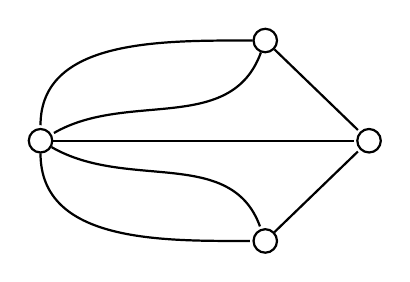
\begin{tikzpicture}[-,>=stealth,shorten >=1pt,auto,node distance=2cm,thick,main node/.style={scale=0.9,circle,draw,font=\sffamily\normalsize}]
            \node[main node] (1) {};
            \node[main node] (2) [below left of=1, xshift = -50] {};
            \node[main node] (3) [below right of=2, xshift = 50] {};
            \node[main node] (4) [right of=2, xshift = 75] {};

            \path[every node/.style={font=\sffamily\small}]
                (1) edge [out=180, in=90] (2)
                (1) edge [out=-110, in=30] (2)
                (2) edge [out=270, in=180] (3)
                (2) edge [out=-30, in=110] (3)
                (2) edge (4)
                (1) edge (4)
                (3) edge (4)
                ;
        \end{tikzpicture}
        \caption{The graph drawn by Euler for the Seven Bridges of Königsberg problem.}
        \label{konigsberg}
    \end{figure}

    Through his analysis, Euler discovered a key insight: for a walk to cross each bridge exactly once and return to the starting point, each landmass must be connected to an even number of bridges. In the case of Königsberg, however, every landmass was connected to an odd number of bridges, making such a walk impossible. Euler's solution, published in 1736, was groundbreaking. It not only answered the Königsberg puzzle but also laid the groundwork for an entirely new field of mathematics: \textit{graph theory}. This area of study has since become fundamental to understanding networks, from transportation systems to social media, and even the internet itself. Thus, from a simple riddle about bridges in a small Prussian city, a new mathematical discipline was born—one that continues to influence the world to this day.

    \begin{frameddefn}{Graph}
        A \textbf{graph} is a mathematical structure $G = (V,E)$, where $V$ is the set of vertices (or nodes) of $G$ and $E$ is the set of edges that link the vertices of $G$.
    \end{frameddefn}

    A graph can be \textbf{directed} or \textbf{undirected}. In a directed graph the edges are \textit{oriented}, meaning that there is difference between the edge $(u,v)$ -- going from $u$ to $v$ -- and the edge $(v,u)$ -- going from $v$ to $u$. Formally, we have that:
    \[E(G) \subseteq V \times V \{ (u,v) \mid u,v \in V(G)\}\]

    In an undirected graph, instead, the edges are \textit{not oriented}, meaning that there not is difference between the edges $(u,v)$ and $(v,u)$. Formally, we have that:
    \[E(G) \subseteq \binom{V(G)}{2} = \{ \{u,v\} \mid u,v \in V(G)\}\]
    \begin{figure}[H]
        \centering


        \begin{tabular}{ccc}
            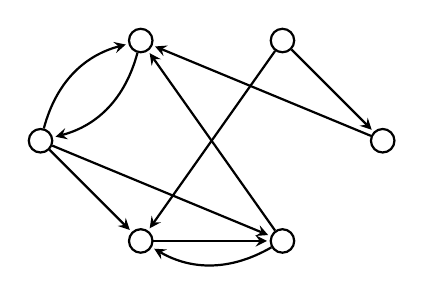
\begin{tikzpicture}[->,>=stealth,shorten >=1pt,auto,node distance=2cm,thick,main node/.style={scale=0.9,circle,draw,font=\sffamily\normalsize}]
                \node[main node] (1) {};
                \node[main node] (2) [below left of=1] {};
                \node[main node] (3) [below right of=2] {};
                \node[main node] (6) [right of=1] {};
                \node[main node] (5) [below right of=6] {};
                \node[main node] (4) [below left of=5] {};
    
                \path[every node/.style={font=\sffamily\small}]
                    (1) edge [bend left](2)
                    (2) edge [bend left] (1)
                    (2) edge (3)
                    (2) edge (4)
                    (3) edge (4)
                    (4) edge [bend left](3)
                    (4) edge (1)
                    (5) edge (1)
                    (6) edge (3)
                    (6) edge (5)
                    ;
            \end{tikzpicture}

            &\qquad\qquad&
            
            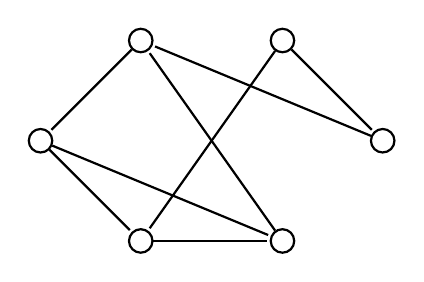
\begin{tikzpicture}[-,>=stealth,shorten >=1pt,auto,node distance=2cm,thick,main node/.style={scale=0.9,circle,draw,font=\sffamily\normalsize}]
                \node[main node] (1) {};
                \node[main node] (2) [below left of=1] {};
                \node[main node] (3) [below right of=2] {};
                \node[main node] (6) [right of=1] {};
                \node[main node] (5) [below right of=6] {};
                \node[main node] (4) [below left of=5] {};
    
                \path[every node/.style={font=\sffamily\small}]
                    (1) edge (2)
                    (2) edge (3)
                    (2) edge (4)
                    (3) edge (4)
                    (4) edge (1)
                    (5) edge (1)
                    (6) edge (3)
                    (6) edge (5)
                    ;
            \end{tikzpicture}
        \end{tabular}

        \caption{A directed graph (left) and an undirected graph (right)}
    \end{figure}

    We observe that the definition of graph that we just gave doesn't allow \textit{multiple edges} between two vertices and \textit{loops}, i.e. edges out-going frm and in-going to the same vertex. When this is the case, we say that the graph is \textbf{simple}. Generally, simple graphs are enough for any model. Sometimes, however, multiple edges and loops are needed -- such as in the Seven Bridges of Königsberg problem. Graphs that allow such edges are called \textbf{multigraphs}.

    \begin{figure}[H]
        \centering
        \begin{tabular}{ccc}
            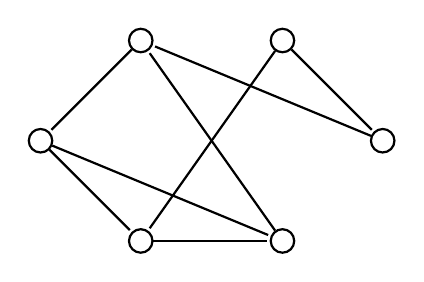
\begin{tikzpicture}[-,>=stealth,shorten >=1pt,auto,node distance=2cm,thick,main node/.style={scale=0.9,circle,draw,font=\sffamily\normalsize}]
                \node[main node] (1) {};
                \node[main node] (2) [below left of=1] {};
                \node[main node] (3) [below right of=2] {};
                \node[main node] (6) [right of=1] {};
                \node[main node] (5) [below right of=6] {};
                \node[main node] (4) [below left of=5] {};
    
                \path[every node/.style={font=\sffamily\small}]
                    (1) edge (2)
                    (2) edge (3)
                    (2) edge (4)
                    (3) edge (4)
                    (4) edge (1)
                    (5) edge (1)
                    (6) edge (3)
                    (6) edge (5)
                    ;
            \end{tikzpicture}

            &\qquad\qquad&
            
            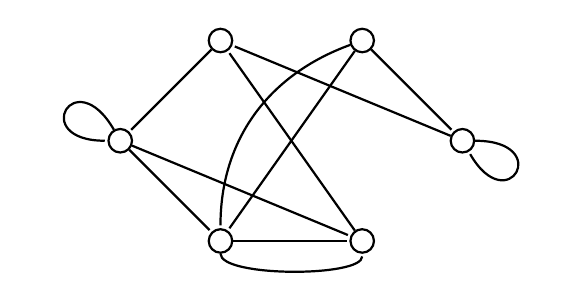
\begin{tikzpicture}[-,>=stealth,shorten >=1pt,auto,node distance=2cm,thick,main node/.style={scale=0.9,circle,draw,font=\sffamily\normalsize}]
                \node[main node] (1) {};
                \node[main node] (2) [below left of=1] {};
                \node[main node] (3) [below right of=2] {};
                \node[main node] (6) [right of=1] {};
                \node[main node] (5) [below right of=6] {};
                \node[main node] (4) [below left of=5] {};
    
                \path[every node/.style={font=\sffamily\small}]
                    (1) edge (2)
                    (2) edge (3)
                    (2) edge (4)
                    (2) edge [loop left, in=180, out=120, min distance=10mm] (2)
                    (3) edge (4)
                    (3) edge [in=-90, out=-90, max distance=3mm] (4)
                    (4) edge (1)
                    (5) edge (1)
                    (5) edge [loop right, in=-60, out=0, min distance=10mm] (5)
                    (6) edge (3)
                    (6) edge [in=90, out=200, min distance=10mm] (3)
                    (6) edge (5)
                    ;
            \end{tikzpicture}
        \end{tabular}
        \caption{A simple graph (left) and a multigraph (right)}
        \label{graph}
    \end{figure}

    From now on, unless stated differently, we'll assume that each graph is \underline{simple} and \underline{undirected}. Moreover, to make notation lighter, we will always assume that $\abs{V(G)} = n, \abs{E(G)} = m$ and that $xy = \{x,y\}$ (or $xy = (x,y)$ for directed graphs). 

    \begin{frameddefn}{Subgraph}
        Let $G$ be a graph. If $H$ is a graph such that $V(H) \subseteq V(G)$ and $E(H) \subseteq E(G)$ then $H$ is a \textbf{subgraph} of $G$, written as $H \subseteq G$. A subgraph $H \subseteq G$ is said to be \textbf{induced} when for all edges $xy \in E(G)$ such that $u,v \in V(H)$ it holds that $xy \in E(H)$.
    \end{frameddefn}

    \begin{figure}[H]
        \centering
        \begin{tabular}{ccc}
            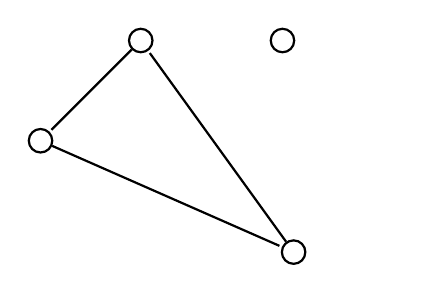
\begin{tikzpicture}[-,>=stealth,shorten >=1pt,auto,node distance=2cm,thick,main node/.style={scale=0.9,circle,draw,font=\sffamily\normalsize}]
                \node[main node] (1) {};
                \node[main node] (2) [below left of=1] {};
                \node[] (3) [below right of=2] {};
                \node[main node] (6) [right of=1] {};
                \node[] (5) [below right of=6] {};
                \node[main node] (4) [below left of=5] {};
    
                \path[every node/.style={font=\sffamily\small}]
                    (1) edge (2)
                    (2) edge (4)
                    (4) edge (1)
                    ;
            \end{tikzpicture}

            &\qquad\qquad&
            
            \begin{tikzpicture}[-,>=stealth,shorten >=1pt,auto,node distance=2cm,thick,main node/.style={scale=0.9,circle,draw,font=\sffamily\normalsize}]
                \node[main node] (1) {};
                \node[main node] (2) [below left of=1] {};
                \node[] (3) [below right of=2] {};
                \node[main node] (6) [right of=1] {};
                \node[] (5) [below right of=6] {};
                \node[main node] (4) [below left of=5] {};
    
                \path[every node/.style={font=\sffamily\small}]
                    (1) edge (2)
                    (4) edge (1)
                    ;
            \end{tikzpicture}
        \end{tabular}
        \caption{Both graphs are a subgraph of the simple graph shown on the left in \Cref{graph}. The left subgraph is induced, while the right one is not.}
    \end{figure}

    We observe that, by definition, if a subgraph $H \subseteq G$ is induced then $H$ is the unique induced subgraph for the vertices $V(H)$. Hence, when talking about an induced graphs we can consider his set of vertices. Given a subset of vertices $X \subseteq V(G)$, we denote with $G[X]$ the unique induced subgraph of $G$ such that $V(G[X]) = X$, where $E(G[X]) = \{xy \in E(G) \mid x,y \in X\}$. 


    \begin{frameddefn}{Adjancency, neighborhood and independence}
        Given a graph $G$ and two nodes $x,y \in V(G)$, we say that $x,y$ are \textbf{adjacent} to each other, written as $x \sim y$, if $xy \in E(G)$. For any edge $xy \in E(G)$, we say that $xy$ is incident to $x$ and $y$. The set of all vertices adjacent to $x$ in $G$ is called \textbf{neighborhood}, written as $N_G(x)$, is defined as:
        \[N_G(x) = \{y \in V(G) \mid x \sim y\}\]

        A subset of vertices $X$ such that for each $x,y \in X$ it holds that $x \not\sim y$ is called \textbf{independent set}.
    \end{frameddefn}
    
    \begin{figure}[H]
        \centering
        \begin{tikzpicture}[-,>=stealth,shorten >=1pt,auto,node distance=2cm,thick,main node/.style={scale=0.9,circle,draw,font=\sffamily\normalsize}]
            \node[main node, fill = BlueLagoon] (1) {};
            \node[main node, fill = Carmine] (2) [below left of=1] {};
            \node[main node, fill = BlueLagoon] (3) [below right of=2] {};
            \node[main node] (6) [right of=1] {};
            \node[main node] (5) [below right of=6] {};
            \node[main node, fill = BlueLagoon] (4) [below left of=5] {};

            \path[every node/.style={font=\sffamily\small}]
                (1) edge (2)
                (2) edge (3)
                (2) edge (4)
                (3) edge (4)
                (4) edge (1)
                (5) edge (1)
                (6) edge (3)
                (6) edge (5)
                ;
        \end{tikzpicture}
        \caption{The blue nodes form the neighborhood of the red node. The red node and the white nodes form an independent set.}
    \end{figure}

    \begin{frameddefn}{Degree}
        Let $G$ be a graph. Given a vertex $x \in V(G)$, the \textbf{degree} of $x$ over $G$ is defined as $\deg_G(x) = \abs{N_G(x)}$. The minimum and maximum degree of $G$ are respectively denoted  as $\delta(G)$ and $\Delta(G)$.
        \[\delta(G) = \min_{x \in V(G)} \deg_G(x)\]
        \[\Delta(G) = \max_{x \in V(G)} \deg_G(x)\]

        We say that a graph is \textbf{k-regular} if $\delta = \Delta = k$, i.e. every node has degree $k$
    \end{frameddefn}

    When the context makes it clear, we'll simply write $\deg(x)$ instead of $\deg_G(x)$. The minimum and maximum degree of a graph are two very powerful theorem-proving tools: large portion of results are proven by reasoning on the degree of each node, often proving that some condition does or does not hold. The most basic result involving the degree of a graph is known as the \textbf{Handshaking lemma}, which can be stated in two equivalent forms. 

    \begin{framedlem}{Handshaking lemma}
        For every graph $G$ it holds that:
        \[\sum_{x \in V(G)} \deg(x) = 2m\]
        Equivalently, for every graph $G$ the number of odd-degree vertices is even.
    \end{framedlem}

    \begin{proof}
        It's easy to see that every edge $xy \in E(G)$ is counted exactly two times through $\deg(x)$ and $\deg(y)$, implying that:
        \[\sum_{x \in V(G)} \deg(x) = 2m\]

        Consider now the subset $X \subseteq V(G)$ containing all the vertices of even degree. We observe that:
        \[2m = \sum_{x \in V(G)} \deg(x) = \sum_{x \in X} \deg(x) + \sum_{x' \in V(G)-X} \deg(x')\]

        Let $a = \sum_{x \in X} \deg(x)$ and $b = \sum_{x' \in X} \deg(x')$. Since the degrees of the vertices in $X$ are even, we know that $a$ is even. Hence, in order for $2m = a +b$ to hold, $b$ must also be even. However, since each degree in $V(G) - X$ is odd, in order for $b$ to be even it must hold that $\abs{V(G)-X}$ is even.
    \end{proof}

    \section{Paths, walks, cycles and trees}

    After discussing the more general concept of subgraph, we can now focus on particular types of structures that can be usually found in graphs. These sub-structures are the real fundamental tool of reasoning for graph properties.

    \begin{frameddefn}{Path}
        A \textbf{path} is a graph $P$ such that $V(P) = \{x_1, \ldots, x_n\}$ and $E(G) = \{x_0x_1, x_1x_2, \ldots, x_{n-1}x_n\}$. The length of a path is defined as the number of edges that form it. A path with $n$ vertices is denoted as $P_n$.
    \end{frameddefn}

    \begin{figure}[H]
        \centering
        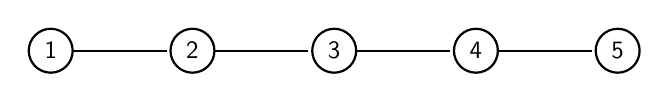
\begin{tikzpicture}[-,>=stealth,shorten >=1pt,auto,node distance=2cm,thick,main node/.style={scale=0.9,circle,draw,font=\sffamily\normalsize}]
            \node[main node] (1) [] {1};
            \node[main node] (2) [right of = 1]{2};
            \node[main node] (3) [right of = 2]{3};
            \node[main node] (4) [right of = 3]{4};
            \node[main node] (5) [right of = 4]{5};

            \path[every node/.style={font=\sffamily\small}]
                (1) edge (2)
                (2) edge (3)
                (3) edge (4)
                (4) edge (5)
                ;
        \end{tikzpicture}
        \caption{The path $P_5$.}
    \end{figure}

    \begin{frameddefn}{Walk}
        Let $G$ be a graph. A \textbf{walk} on $G$ is defined as a sequence $x_0 e_1 x_1 e_2 \ldots e_{k-1} e_k x_k$ where $x_0, \ldots, x_k \in V(G)$ and $e_1, \ldots, e_k \in E(G)$. The length of a walk is defined as the number of edges that form it.
    \end{frameddefn}
    
    When the first and last vertices are equal, i.e. $x_0 = x_k$, we say that the walk is \textbf{closed}. We observe that, by definition, a walk allows edges and vertices to be repeated in the sequence.  When no vertices in a walk are repeated, the walk corresponds to a path.
    
    \begin{figure}[H]
        \centering
        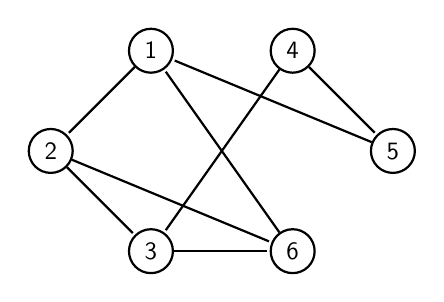
\begin{tikzpicture}[-,>=stealth,shorten >=1pt,auto,node distance=2cm,thick,main node/.style={scale=0.9,circle,draw,font=\sffamily\normalsize}]
            \node[main node] (1) {1};
            \node[main node] (2) [below left of=1] {2};
            \node[main node] (3) [below right of=2] {3};
            \node[main node] (6) [right of=1] {4};
            \node[main node] (5) [below right of=6] {5};
            \node[main node] (4) [below left of=5] {6};

            \path[every node/.style={font=\sffamily\small}]
                (1) edge (2)
                (2) edge (3)
                (2) edge (4)
                (3) edge (4)
                (4) edge (1)
                (5) edge (1)
                (6) edge (3)
                (6) edge (5)
                ;
        \end{tikzpicture}
        \caption{The sequence $1 \{1,2\} 2 \{2,6\} 6 \{6,1\} 1 \{1,5\} 5$ forms a walk on $G$, but not a path. The sequence  $1 \{1,2\} 2 \{2,6\} 6 \{6,3\} 3 \{3,4\} 4$, instead, forms a path on $G$.}
    \end{figure}

    \begin{framedprop}[label=paths_walks]{Paths and walks}
        Let $G$ be a graph. Given the vertices $x,y \in V(G)$, there is a path from $x$ to $y$ if and only if there is a walk from $x$ to $y$.
    \end{framedprop}

    \begin{proof}
        Since every path is also a walk, the first direction is trivial. Let $W = x_0 e_1 x_1 e_2 \ldots$ $e_{k-1} e_k x_k$ be the shortest walk. i.e the one with minimum length, such that $x = x_0$ and $y = x_k$. By way of contradiction, suppose that $W$ is not a path. Hence, at least one edge in $W$ must repeat at least once. Let $i,j \in [k]$ be two indices such that $e_i = e_j$. Then, the following sequence $W'$ is a walk from $x$ to $y$ with fewer edges than $W$, raising a contradiction. Hence, $W$ must be a path.
        \[W' = x_0 e_1 x_1 e_2 \ldots e_i x_i e_{j+1} x_{j+1} e_{j+2} \ldots e_{k-1} e_k x_k\]
    \end{proof}

    \begin{framedprop}[label=delta_path]{}
        The longest path in any graph has length at least $\delta$.
    \end{framedprop}

    \begin{proof}
        If $\delta = 1$ then the longest path is trivially made by one single edge. Suppose now that $\delta \geq 2$, implying that there are at least two vertices in $G$. Let $P$ be the longest path in $G$ and let $x_1, \ldots, x_k$ be its vertices.

        \textbf{Claim:} $N(x_k) \subseteq \{x_1, \ldots, x_{k-1}\}$.

        \begin{proof}
            By way of contradiction, suppose that there is a vertex $x' \in N(x_k)$ such that $x' \notin \{x_1, \ldots, x_{k-1}\}$. Then, since $x_k \sim x'$, there must be an edge $x_k x'$, implying that the path $P \cup x_kx'$ is longer than $P$, raising a contradiction. 
        \end{proof}

        Through the claim we easily conclude that $\delta \leq \abs{N(x_k)} \leq k$, meaning that $P$ has length at least $\delta$.
    \end{proof}

    \begin{frameddefn}{Cycle}
        A cycle is a graph $C$ such that $V(C) = \{x_1, \ldots, x_n\}$ and $E(G) = \{x_0x_1, x_1x_2, \ldots,$ $x_{n-1}x_n, x_nx_1\}$. The length of a cycle is defined as the number of edges that form it. A cycle with $n$ vertices is denoted as $C_n$.
    \end{frameddefn}

    \begin{figure}[H]
        \centering
        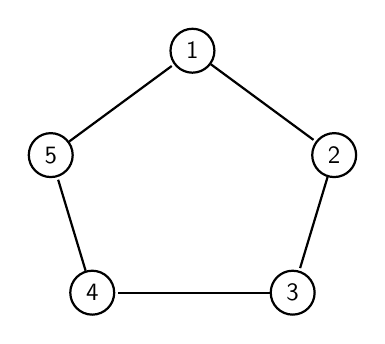
\begin{tikzpicture}[-,>=stealth,shorten >=1pt,auto,node distance=2cm,thick,main node/.style={scale=0.9,circle,draw,font=\sffamily\normalsize}]
            \node[] (x) {};
            \node[main node] (1) [above of = x] {1};
            \node[main node] (2) [right of = x, yshift=15]{2};
            \node[main node] (3) [below right of = x]{3};
            \node[main node] (4) [below left of = x]{4};
            \node[main node] (5) [left of = x, yshift=15]{5};

            \path[every node/.style={font=\sffamily\small}]
                (1) edge (2)
                (2) edge (3)
                (3) edge (4)
                (4) edge (5)
                (5) edge (1)
                ;
        \end{tikzpicture}
        \caption{The cycle $C_5$.}
    \end{figure}

    Given a graph $G$ and a cycle $C$, we say that the edge $xy$ is a \textbf{chord} of $C$ if $x,y \in V(C)$ and $xy \in E(G-C)$, i.e. it is an edge that splits the graph into two parts.

    \begin{framedprop}[label={delta_cycle}]{}
        In any graph such that $\delta \geq 2$ there is a cycle of length at least $\delta + 1$.
    \end{framedprop}

    \begin{proof}
        Let $P$ be the longest path in $G$ and let $x_1, \ldots, x_k$ be its vertices. Through an argument equal to the claim of \Cref{delta_path}, we know that $N(x_k) \subseteq \{x_1, \ldots, x_{k-1}\}$. Let $i \in [k-1]$ be the minimal index such that $x_i \in N(x_k)$. Since every neighbor of $x_k$ must be inside $P$ and the graph is simple, it must hold that $i \geq \delta$, meaning that the vertices $x_i, x_{i+1}, \ldots, x_{k-1}, x_k, x_i$ form the cycle $C_{i+1}$.
    \end{proof}

    \begin{frameddefn}{Connectivity, components and distance}
        Let $G$ be a graph. Two nodes $x,y \in V(G)$ are said to be linked if there is a path from $x$ to $y$. If every pair of nodes in $G$ is linked, we say that $G$ is \textbf{connected}. If a connected subgraph $H$ of $G$ is maximal -- meaning that no other edges can be added to it while preserving connectivity -- $H$ is called \textbf{component} of $G$. The \textbf{distance} $\dist_G(x,y)$ between two nodes $x,y$ is the length of the shortest path connecting them.
    \end{frameddefn}

    \begin{figure}[H]
        \centering
        \begin{tabular}{ccc}
            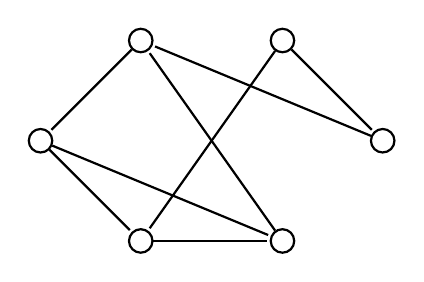
\begin{tikzpicture}[-,>=stealth,shorten >=1pt,auto,node distance=2cm,thick,main node/.style={scale=0.9,circle,draw,font=\sffamily\normalsize}]
                \node[main node] (1) {};
                \node[main node] (2) [below left of=1] {};
                \node[main node] (3) [below right of=2] {};
                \node[main node] (6) [right of=1] {};
                \node[main node] (5) [below right of=6] {};
                \node[main node] (4) [below left of=5] {};
    
                \path[every node/.style={font=\sffamily\small}]
                    (1) edge (2)
                    (2) edge (3)
                    (2) edge (4)
                    (3) edge (4)
                    (4) edge (1)
                    (5) edge (1)
                    (6) edge (3)
                    (6) edge (5)
                    ;
            \end{tikzpicture}

            &\qquad\qquad&
            
            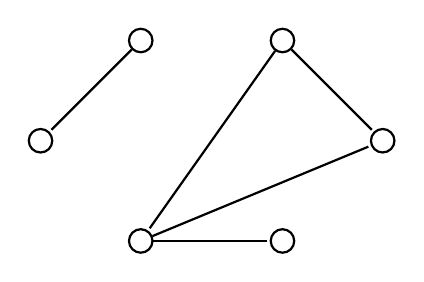
\begin{tikzpicture}[-,>=stealth,shorten >=1pt,auto,node distance=2cm,thick,main node/.style={scale=0.9,circle,draw,font=\sffamily\normalsize}]
                \node[main node] (1) {};
                \node[main node] (2) [below left of=1] {};
                \node[main node] (3) [below right of=2] {};
                \node[main node] (6) [right of=1] {};
                \node[main node] (5) [below right of=6] {};
                \node[main node] (4) [below left of=5] {};
    
                \path[every node/.style={font=\sffamily\small}]
                        (1) edge (2)
                        (3) edge (4)
                        (6) edge (3)
                        (6) edge (5)
                        (3) edge (5)
                    ;
            \end{tikzpicture}
        \end{tabular}
        \caption{A connected graph (left) and a disconnected graph (right). The connected graph has an unique component, while the disconnected graph has two components.}
    \end{figure}

    \begin{framedlem}[label={cycle_conn}]{}
        Let $G$ be a graph. If $G$ is connected and $C$ is a cycle in $G$ then for all $e \in E(C)$ it holds that $G - \{e\}$ is still connected.
    \end{framedlem}

    \begin{proof}
        Fix an edge $e \in E(C)$. Let $P = x_0 e_1 x_1 \ldots e_k x_k$ be a path in $G$ from $x$ to $y$. If $e \notin E(P)$ then $P$ is also a path in $G - \{e\}$, preserving the connectivity of $x$ and $y$. Suppose now that $e \in E(P)$. Given $C = z_0 f_1 z_1 \ldots f_v z_v$, without loss of generality assume that $e = e_i = f_1$. Then, the following sequence $W$ is a walk from $x$ to $y$ in $G - \{e\}$ -- we cannot be sure that $W$ is a path since $P$ may intersect $C$ on multiple edges.
        \[W =  x_0 e_1 x_1 \ldots x_i f_v z_{v-1} \ldots f_2 z_2 e_{i+1} x_{i+1} \ldots e_k x_k\]

        By \Cref{paths_walks}, we know that since $W$ is a walk from $x$ to $y$ in $G- \{e\}$ there must also be a path from $x$ to $y$ in $G-\{e\}$, preserving connectivity.
    \end{proof}

    \begin{frameddefn}{Tree}
        A \textbf{tree} is an connected acyclic subgraph. Any vertex in a tree with degree 1 is called leaf. A rooted tree is a tree with a chosen node called \textbf{root}. If every component of a graph is a tree, the graph is referred to as a \textbf{forest}.
    \end{frameddefn}

    \begin{figure}[H]
        \centering
        \begin{tikzpicture}[-,>=stealth,shorten >=1pt,auto,node distance=2.5cm,thick,main node/.style={scale=0.9,circle,draw,font=\sffamily\normalsize}]
            \node[main node] (1) {};
            \node[main node, fill = Carmine] (2) [right of=1] {};
            \node[main node] (3) [below right of=2] {};
            \node[main node] (4) [above of=1] {};
            \node[main node] (5) [above of=2] {};
            \node[main node] (6) [above left of=1] {};
            \node[main node] (7) [below left of=1] {};

            \path[every node/.style={font=\sffamily\small}]
                (6) edge (1)
                (6) edge (4)
                (1) edge (5)
                (1) edge (2)
                (2) edge (3)
                (1) edge (7)
            ;
        \end{tikzpicture}
        \caption{A rooted tree. The red node has been chosen as the root.}
    \end{figure}

    When the tree is rooted in $r \in V(T)$, we often use the concept of \textbf{ancestor} and \textbf{parent}. Given two nodes $a,x \in V(T)$, we say that $a$ is an ancestor of $x$ if $x$ lies on a path from $r$ to $x$. If $p$ is an ancestor of $x$ and $px \in E(T)$, we say that $p$ is the parent of $x$. The \textbf{least common ancestor (LCA)} between two vertices $x,y \in V(T)$ is the ancestor $z \in V(T)$ shared by $x$ and $y$ that minimizes the value of $\dist(r,z)$.  We observe that every pair of vertices of a tree must have a LCA since the root is an ancestor of every node.


    \begin{framedthm}[label={tree_defs}]{Equivalent definitions of tree}
        Given a graph $T$, the following statements are equivalent:
        \begin{enumerate}
            \item $T$ is a tree
            \item Every vertex pair of $T$ is connected by an unique path
            \item $T$ is minimally connected
            \item $T$ is maximally acyclic
        \end{enumerate}
    \end{framedthm}

    \begin{proof}
        We'll proceed by proving a chain of implications.
        \begin{itemize}
            \item[$1 \implies 2$] Without loss of generality, assume that every pair of nodes has at least one path, since otherwise $T$ is not connected, hence not a tree. Suppose now that there are two vertices $x,y \in V(T)$ that have at least two different paths $P, Q$ from $x$ to $y$. While traversing $P$ from $x$ to $y$, let $z$ be the first node such that $z \in V(P) \cap V(Q)$. Similarly, let $w \in V(P) \cap V(Q)$ be the first node encountered while traversing $Q$ from $y$ to $x$. We observe that since $x,y \in V(P) \cap V(Q)$, the vertices $z,w$ always exist. Given the subpath $P' \subseteq P$ from $w$ to $z$ and the subpath $Q' \subseteq Q$ from $z$ to $w$, the graph $Q' \cup P'$ is a cycle in $T$, meaning that $T$ cannot be a tree. By contrapositive, we get that if $T$ is a tree then every pair of vertices is connected by an unique path.
            
            \item[$2 \implies 3$] Suppose that every vertex pair of $T$ is connected by an unique path. Then, $T$ is clearly connected. By way of contradiction, suppose that there is an edge $e \in E(G)$ such that $T-\{e\}$ is still connected. Then, the edge $e$ must be part of at least one of the unique paths connecting two nodes, meaning that such path cannot exist inside $T - \{e\}$, implying that it is not connected. Hence, $T$ must be minimally connected.
            
            \item[$3 \implies 4$] Suppose that $T$ is minimally connected but not maximally acyclic. By way of contradiction, suppose that $T$ has a cycle. Then, by \Cref{cycle_conn} we know that we can remove an edge of the cycle from $T$ and keep it connected, contradicting the fact that $T$ is minimally connected. Hence, $T$ must be acyclic. Pick two vertices $x,y \in V(T)$. Since $T$ is connected, we know that there is a path $P$ connecting $x$ to $y$. Then, if we were to add the edge $xy$, the subgraph $P \cup \{xy\}$ would be a cycle in $T \cup \{xy\}$. Thus, $T$ is maximally acyclic.
            
            \item[$4 \implies 1$] Suppose that $T$ is maximally acyclic. Fix a pair of vertices $x,y \in V(T)$. Since $T$ is maximally acyclic, we know that adding the edge $xy$ makes $T \cup \{xy\}$ cyclic. Let $C$ be the cycle in $T \cup \{xy\}$ containing $xy$. Then, $C - \{xy\}$ must be a path in $T$ from $x$ to $y$.
        \end{itemize}
    \end{proof}

    \newpage

    \begin{framedlem}{}
        Let $T$ be a tree. Then:
        \begin{enumerate}
            \item If $T$ has at least two nodes then $T$ has at least a leaf.
            \item If $x \in V(T)$ is a leaf then $T-\{x\}$ is still a tree
        \end{enumerate}
    \end{framedlem}

    \begin{proof}

        \quad

        \begin{enumerate}
            \item By way of contradiction, suppose that $T$ is a tree without leaves. Then, we have that $\delta \geq 2$. However, by \Cref{delta_cycle}, in $T$ there must be a cycle with length at least $\delta+1$, contradicting the very definition of tree. Hence, $T$ must have at least a leaf.
    
            \item Let $x$ be a leaf of $T$. Since $T$ is acyclic, $T-\{x\}$ is also clearly acyclic. By way of contradiction, suppose that $T-\{x\}$ is not connected. Then, there are at least two vertices $u,v \in V(T-\{x\})$ for which there is a path $P$ between them in $T$ but not in $T-\{x\}$. Since by removing $x$ the vertices $u,v$ became disconnected, the vertex $x$ must lie on $P$. Moreover, since $u, v \neq x$, the vertex $x$ must be an internal node of the path, meaning that it must have degree 2, contradicting the very definition of leaf. 
        \end{enumerate}
    \end{proof}

    \begin{frameddefn}{Spanning tree}
        Given a graph $G$, we say that $T \subseteq G$ is a \textbf{spanning tree} of $G$ if $T$ is a tree and $V(T) = V(G)$.
    \end{frameddefn}

    \begin{figure}[H]
        \centering
        \begin{tabular}{ccc}
            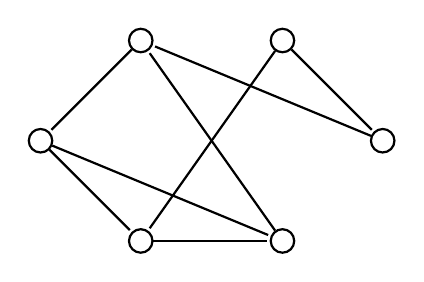
\begin{tikzpicture}[-,>=stealth,shorten >=1pt,auto,node distance=2cm,thick,main node/.style={scale=0.9,circle,draw,font=\sffamily\normalsize}]
                \node[main node] (1) {};
                \node[main node] (2) [below left of=1] {};
                \node[main node] (3) [below right of=2] {};
                \node[main node] (6) [right of=1] {};
                \node[main node] (5) [below right of=6] {};
                \node[main node] (4) [below left of=5] {};
    
                \path[every node/.style={font=\sffamily\small}]
                    (1) edge (2)
                    (2) edge (3)
                    (2) edge (4)
                    (3) edge (4)
                    (4) edge (1)
                    (5) edge (1)
                    (6) edge (3)
                    (6) edge (5)
                    ;
            \end{tikzpicture}

            &\qquad\qquad&
            
            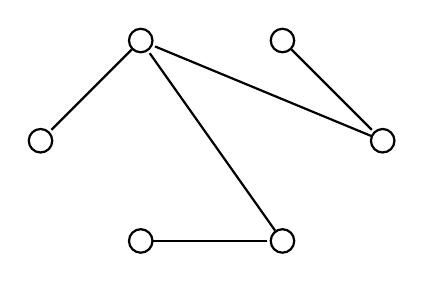
\begin{tikzpicture}[-,>=stealth,shorten >=1pt,auto,node distance=2cm,thick,main node/.style={scale=0.9,circle,draw,font=\sffamily\normalsize}]
                \node[main node] (1) {};
                \node[main node] (2) [below left of=1] {};
                \node[main node] (3) [below right of=2] {};
                \node[main node] (6) [right of=1] {};
                \node[main node] (5) [below right of=6] {};
                \node[main node] (4) [below left of=5] {};
    
                \path[every node/.style={font=\sffamily\small}]
                        (1) edge (2)
                        (3) edge (4)
                        (4) edge (1)
                        (5) edge (1)
                        (6) edge (5)
                    ;
            \end{tikzpicture}
        \end{tabular}
        \caption{A graph (left) and one of its spanning trees (right)}
    \end{figure}

    \begin{framedlem}{}
        Every connected graph has a spanning tree.
    \end{framedlem}

    \begin{proof}
        If $G$ is a tree then clearly it is its own spanning tree. Suppose now that $G$ is a connected graph that is not a tree, meaning that it is acyclic.  Then, through \Cref{delta_cycle}, we can keep removing the edges $e_1, \ldots, e_k$ from every cycle of $G$ until we reach a minimally connected subgraph $T$ such that $V(T) = V(G)$. By \Cref{tree_defs}, we know that $T$ must be a tree.
    \end{proof}

    \begin{framedthm}{}
        Let $T$ be a connected graph. Then, $T$ is a tree if and only if it has $n-1$ edges.
    \end{framedthm}

    \begin{proof}
        We proceed by induction on $n$. If $n = 1$ then $T$ is trivially the tree with 0 edges. If $n > 1$, instead, through the previous lemma we know that $T$ must have at least a leaf $x \in V(T)$ for which $T-\{x\}$ is still a tree. By inductive hypothesis, we know that $T-\{x\}$ has $n-2$ edges. Hence, by adding the unique edge incident to $x$, we get that $T$ has $n-1$ edges.

        Vice versa, by way of contradiction, suppose that $T$ is connected, has $n-1$ edges but that it is not acyclic. Then, through the previous lemma we know that $T$ must have a spanning tree $T'$. Moreover, since $T$ has a cycle and $T'$ does not, we know that $T'$ must have fewer edges than $T$. However, we have just proven that every tree must have $n-1$ edges. Hence, we get that $n-1 = \abs{E(T')} < \abs{E(T)} = n-1$, which is a contradiction. Hence, $T$ must also be acyclic.
    \end{proof}

    \section{Complete graphs and bipartite graphs}

    \begin{frameddefn}{Complete graph}
        A \textbf{complete graph} is a graph where every pair of vertices is adjacent to each other. A complete graph with $n$ vertices in denoted as $K_n$. An induced subgraph that is complete is called \textbf{clique}.
    \end{frameddefn}
    
    \begin{figure}[H]
        \centering
        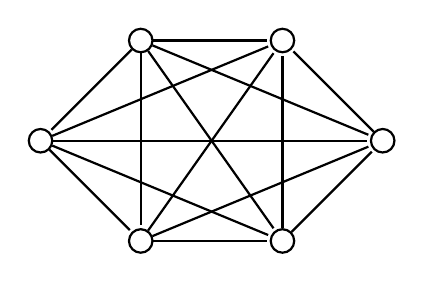
\begin{tikzpicture}[-,>=stealth,shorten >=1pt,auto,node distance=2cm,thick,main node/.style={scale=0.9,circle,draw,font=\sffamily\normalsize}]
            \node[main node] (1) {};
            \node[main node] (2) [below left of=1] {};
            \node[main node] (3) [below right of=2] {};
            \node[main node] (6) [right of=1] {};
            \node[main node] (5) [below right of=6] {};
            \node[main node] (4) [below left of=5] {};

            \path[every node/.style={font=\sffamily\small}]
                (1) edge (2)
                (1) edge (3)
                (1) edge (4)
                (1) edge (5)
                (1) edge (6)

                (2) edge (3)
                (2) edge (4)
                (2) edge (5)
                (2) edge (6)

                (3) edge (4)
                (3) edge (5)
                (3) edge (6)

                (4) edge (5)
                (4) edge (6)

                (5) edge (6)
                ;
        \end{tikzpicture}

        \caption{The complete graph $K_6$}
    \end{figure}

    \begin{frameddefn}{Bipartite graph}
        A \textbf{bipartite graph} is a graph with a subset of vertices $X \subseteq V(G)$ such that for every edge $\{u,v\} \in E(G)$ it holds that $u \in X$ and $v \in V(G)- X$. Equivalently, we have that both $X$ and $V(G)-X$ are independent sets.
    \end{frameddefn}

    \begin{figure}[H]
        \centering
        \resizebox{0.175\textwidth}{!}{
            \begin{tikzpicture}[-,>=stealth,shorten >=1pt,auto,node distance=2cm,thick,main node/.style={scale=1,circle,draw,font=\sffamily\normalsize}, rotate=90,transform shape]
                \node[main node] (1) [fill = Carmine,]{};
                \node[main node] (2) [fill = Carmine,right of=1] {};
                \node[main node] (3) [fill = Carmine,right of=2] {};
                \node[main node] (4) [fill = Carmine,right of=3] {};
                \node (5) [below right of=1] {};
                \node[main node] (6) [fill = BlueLagoon,below left of=5] {};
                \node[main node] (7) [fill = BlueLagoon,right of=6] {};
                \node[main node] (8) [fill = BlueLagoon,right of=7] {};
                \node[main node] (9) [fill = BlueLagoon,right of=8] {};

                \path[every node/.style={font=\sffamily\small}]
                        (1) edge (6)
                        (1) edge (9)
                        (2) edge (8)
                        (3) edge (6)
                        (3) edge (7)
                        (4) edge (8)
                        (4) edge (9)
                    ;
            \end{tikzpicture}
        }

        \caption{The red and blue nodes form a bipartition of the graph.}
    \end{figure}

    It's easy to see that no complete graph can be bipartitioned since it's impossible to separates the nodes into two independent sets. In fact, by definition, cliques are the very opposite of the concept of independent set. Through the following lemma we can extend the claim on complete graphs to cliques: if $G$ contains a clique of any cardinality then $G$ cannot be bipartitioned.

    \begin{framedprop}{}
        $G$ is bipartite if and only if every subgraph of $G$ is bipartite
    \end{framedprop}

    \begin{proof}
        The converse implication trivially holds. Let $H$ be a subgraph of $G$. Then, any bipartition $(X, V(G)-X)$ of $G$ induces a bipartition $(X \cap V(H), V(H)- X)$ over $H$. 
    \end{proof}

    \begin{framedlem}{}
        $G$ is bipartite if and only if every component of $G$ is bipartite
    \end{framedlem}
    
    \begin{proof}
        The direct implication trivially follows from the previous proposition. Given the components $H_1, \ldots, H_k$ of $G$, let $(X_1, V(H_1)- X_1), \ldots, (X_k, V(H_k)-X_k)$ be the bipartitions of the components. Then, since each component is by definition disjoint from the others, the pair $\rbk{X, V(G)-X}$ where $X = \bigcup_{i \in [k]} X_i$ is a bipartition of $G$.
    \end{proof}

    We observe that the above characterizations of bipartite graphs are useful but still \curlyquotes{weak}. A stronger characterization can be achieved through the following theorem. Given a path $P$ and two vertices $x,y \in V(P)$, we denote the subpath of $P$ from $x$ to $y$ with $xPy$.

    \begin{framedthm}[label={bip_cycle}]{}
        $G$ is bipartite if and only if it doesn't contain odd cycles.
    \end{framedthm}

    \begin{proof}
        Through the above proposition, it's sufficient to prove that for all $k \in \N$, $C_{2k+1}$ is not bipartite. Fix $k \in \N$. By way of contradiction, suppose that there is bipartition $(X, V(G)-X)$ of $C_{2k+1}$. Let $x_1, \ldots, x_{2k+1} x_1$ be the edges of $C_{2k+1}$. Without loss of generality, assume that $x_1 \in X, x_2 \notin X, x_3 \in X, \ldots, x_{2k} \notin X$. Then, if $x_{2k+1} \in X$ then $x_{2k+1}x_1 \subseteq X$, while if $x_{2k+1} \notin X$ then $x_{2k}x_{2k+1} \subseteq V(G)-X$. In both cases, we get that the pair cannot be a bipartition.

        Vice versa, suppose that $G$ is not bipartite. Then, through the previous lemma at least one component $H$ of $G$ is not bipartite. Let $T$ be a spanning tree of $H$ and fix $r \in V(T)$ as its root. Let $X = \{x \in V(T) \mid \dist_T(r,x) \text{ is even}\}$. By definition, $(X, V(T)-X)$ for a bipartition of $T$. Hence, since $T$ is bipartite but $H$ isn't, there must be an edge $xy \in E(H)$ such that either $x,y \in X$ or $x,y \notin X$. Let $P_x$ and $P_y$ respectively be the paths in $T$ from $x$ to $r$ and from $y$ to $r$. Let $z$ be the LCA of $x$ and $y$ in $T$.

        \textbf{Claim:} $C = z P_x x \cup z P_y y \cup xy$ is an odd cycle

        \begin{proof}[Proof of the claim.]
            Since either $x,y \in X$ or $x,y \notin X$ holds, we know that $\dist(r,x)$ and $\dist(r,y)$ must be either both even or both odd. Hence, the lengths of $P_x$ and $P_y$ must share the same parity. Moreover, since $z$ is the LCA of $x$ and $y$ w have that $r P_x z = rP_y z$. Thus, the lengths of $z P_x x$ and $z P_y y$ must also share the same parity. This concludes that $z P_x x \cup z P_y y \cup xy$ must be an odd cycle.
        \end{proof}

        Since $C$ is an odd cycle and it is a subgraph of $T$, and thus of $G$, we conclude that $G$ contains an odd cycle.
    \end{proof}

    \section{Eulerian tours and Hamiltonian paths}

    At the start of this chapter, we introduced the Seven Bridges of Königsberg problem, which led to the emergence of graph theory as a branch of combinatorics. In modern graph theory, the problem is formalized through the concept of \textit{Eulerian tour}.

    \begin{frameddefn}{Eulerian tour}
        An Eulerian tour over a graph $G$ is closed walk that traverses every edge of $G$ exactly once.
    \end{frameddefn}

    To solve the problem, \textcite{konigsberg} proved the following theorem, which implies that the answer is \curlyquotes{no} since the multigraph that models the problem contains some odd-degree vertices.

    \begin{framedthm}{Euler's theorem}
        A graph (or multigraph) has an Eulerian tour if and only if $G$ is connected and every vertex has even degree
    \end{framedthm}

    \begin{proof}
        By way of contradiction, suppose that $G$ has an Eulerian tour $W$. By way of contradiction, suppose that $G$ is not connected. Then, we get an easy contradiction: if $G$ is disconnected then $W$ cannot traverse every edge of the graph. Hence, $G$ must be connected. Again, by way of contradiction suppose that $G$ has at least one odd-degree vertex $x \in V(G)$. Let $\deg(x) = 2k+1$. Since $W$ is a closed walk, we can assume without loss of generality that $x$ is the first vertex of the walk. When traversing $W$ starting from $x$, one of the edges incident to $x$ is crossed, hence we have $2k$ incident edges left. Every time the tour returns to $x$, two edges are crossed -- one in-going and one out-going. Hence, in order to cover all the edges, the tour has to return to $x$ for $k$ times. However, this implies that there are no more edges left to close the tour on $x$, raising a contradiction. Hence, the vertex $x$ cannot exist.
        
        Vice versa, assume that $G$ is connected and every vertex has even degree. Let $W = x_0 e_1 x_1 \ldots e_k x_k$ be the longest walk over $G$ with no repeating edges.

        \textbf{Claim 1:} $x_k = x_0$, i.e. $W$ is a closed walk

        \begin{proof}[Proof of Claim 1.]
            By way of contradiction, suppose that $x_k \neq x_0$. Let $2v+1$ be the number of edges incident to $x_k$ in $W$ -- one edge is given by $e_k$ while $2v$ edges are given by edges needed to cross the other $v$ the vertices $x_{i_{1}}, \ldots, x_{1_v}$ such that $x_i = x_k$. Since $x_k$ has even degree, we know that there must be another edge $\{x_k, y\} \in E(G-W)$, implying that $W \cup \{x_k,y\}$ is walk longer than $W$, which is absurd.
        \end{proof}

        \textbf{Claim 2: } $W$ contains every edge of $G$
        
        \begin{proof}[Proof of Claim 2.]
            By way of contradiction, suppose that that there is an edge $uv \in E(G-W)$. Fix $i \in [k]$. By connectivity of $G$, we know that there must be a path $P$ disjoint from $x_i$ to $u$ or from $x_i$ to $v$. Without loss of generality, assume that $P$ is a path from $x_i$ to $u$. Since $uv \notin E(W)$, there must be an edge $x_jy \in E(P-W)$ outgoing from $W$. Since $W$ is a closed walk, we can assume  without loss of generality that $x_j$ is the first (and last) vertex of the walk. Then, the walk $W \cup x_jy$ is walk that doesn't repeat any vertices longer than $W$, raising a contradiction.
        \end{proof}

        Through the two claims, we conclude that $W$ is an Eulerian tour.
    \end{proof}

    As a corollary to Euler's theorem, we get that the problem that asks to determine the existence of an Eulerian tour inside the graph lies in the intersection $\mathsf{NP} \cap \mathsf{coNP}$ since the theorem gives us a polynomially verifiable condition both for existence and non-existence of the tour. In fact, as many problems that lie in this intersection, the problem actually lies in the class $\mathsf{P}$.

    Another very interesting concept similar to Eulerian tours was formulated by Hamilton: closed walks that touch every node exactly once instead of every edge exactly once. We observe that this condition implies that the closed walk is nothing more than the subgraph $P_n$. Even though they are similar in concept, finding an \textbf{Hamiltonian path} inside a graph is an $\mathsf{NP}$-hard problem, making it intractable. A variant of this concept is the \textbf{Hamiltonian cycle}, i.e. a cycle that goes through all the nodes of a graph. The decision of existence of Hamiltonian cycles is also $\mathsf{NP}$-hard.

    \begin{frameddefn}{Hamiltonian paths and cycles}
        An Hamiltonian path over a graph $G$ is a subgraph $P_n \subseteq G$. An Hamiltonian cycle over a graph $G$ is a subgraph $C_n \subseteq G$.
    \end{frameddefn}

    When some conditions are met, an Hamiltonian cycle (hence also an Hamiltonian path) is guaranteed to exist. For instance, \textcite{dirac} formulated the following theorem.

    \begin{framedthm}{Dirac's theorem}
        Let $G$ be a graph. If $\delta \geq \frac{n}{2}$ then there is an Hamiltonian cycle in $G$.
    \end{framedthm}

    \begin{proof}
        First of all, we show that Dirac's condition forces the graph to be connected.

        \textbf{Claim 1:} $G$ is connected

        \begin{proof}[Proof of Claim 1.]
            By way of contradiction, suppose that $G$ is not connected. Then, $G$ has at least two components. Hence, the smallest component $H$ of $G$ can have at most $\frac{n}{2}$ edge. However, since $\delta \geq \frac{n}{2}$, each node $x \in H$ must have at least $\frac{n}{2}$ neighbors. Thus, since $\{x\} \cup N(x) \subseteq H$, we get that $H$ must have at least $\frac{n}{2}+1$ nodes, raising a contradiction.
        \end{proof}

        Let $P$ be the longest path on $G$ an let $x_0, \ldots, x_k$ be its vertices. 

        \textbf{Claim 2:} There is an index $v$ such that $x_0, x_{v}, x_{v+1}, \ldots, x_{k-1}, x_k, x_{v-1}, x_{v-2}, \ldots, x_1, x_0$ is a cycle

        \begin{proof}[Proof of Claim 2.]
            Using the same argument as \Cref{delta_path}, we know that $N(x_0), N(x_k) \subseteq \{x_0, \ldots, x_k\}$. Let $I_0$ and $I_k$ be defined as:
            \[I_0 = \{i \mid 1 \leq i \leq k, x_i \in N(x_0)\} \qquad\qquad I_k = \{i \mid 1 \leq i \leq k, x_{i-1} \in N(k)\}\]

            Since $\delta \geq \frac{n}{2}$, we know that $\frac{n}{2} \leq \abs{I_0}, \abs{I_k} \leq n-1$, by the pigeonhole principle there must be at least one index $v \in I_0 \cap I_k$, meaning that $x_0 \sim x_v$ and $x_k \sim x_{v-1}$. Thus, the sequence of nodes $x_0, x_{v}, x_{v+1}, \ldots, x_{k-1}, x_k, x_{v-1}, x_{v-2}, \ldots, x_1, x_0$ is a cycle.
        \end{proof}

        Let $C$ be the cycle given by $x_0, x_{v}, x_{v+1}, \ldots, x_{k-1}, x_k, x_{v-1}, x_{v-2}, \ldots, x_1, x_0$. By way of contradiction, suppose that $C$ has less than $n$ nodes. Given $y \in V(G-C)$, by connectivity of $G$ there must be an index $i$ for which there is a path $P$ connecting $x_i$ and $y$. However, this implies that the following path
        \[P \cup x_ix_{i+1} \cup \ldots \cup x_kx_0 \cup \ldots \cup x_{i-2}x_{i-1}\]
        is longer than $P$, raising a contradiction. Hence, $C$ must be an Hamiltonian cycle.
    \end{proof}

    We observe that Dirac's condition, i.e. $\delta \geq \frac{n}{2}$ is actually optimal, meaning that we cannot find a better lower bound that guarantees the existence of an Hamiltonian cycle: there are many graphs with $\delta = \frac{n}{2} - 1$ for which there is no Hamiltonian cycle.

    \section{Solved exercises}

    \begin{framedprob}{}
        For any graph $G$, prove that at least two vertices have the same degree.
    \end{framedprob}

    \begin{proof}[Solution]
        By way of contradiction, suppose that no vertices share the same degree. Then, the function $\deg : V \to \{0,\ldots, n-1\}$ must be bijective, implying that there are two vertices $u,v \in V$ such that $\deg(u) = 0$ and $\deg(v) = n-1$, which is absurd since there should both be and not be an edge between $u$ and $v$. Hence, at least two vertices must share have the same degree. 
    \end{proof}

    \begin{framedprob}{}
        Show that the components of a graph parition its vertex set.
    \end{framedprob}

    \begin{proof}[Solution]
        Let $G$ be a graph. For each vertex $v$ of $G$, we denote its compinent with $\mathrm{comp}(v)$. Since each node can reach itself, we get that $v \in \mathrm{comp}(v)$, implying that:
        \[V(G) = \bigcup_{v \in V(G)} \mathrm{comp}(v)\]

        Consider now any pair of vertices $x,y \in V(G)$. We observe that if $\mathrm{comp}(v) = \mathrm{comp}(y)$ then $\mathrm{comp}(v) \cap \mathrm{comp}(y) \neq \varnothing$ trivially holds since at least $x$ and $y$ lie in the intersection. Vice versa, suppose that $\mathrm{comp}(v) \cap \mathrm{comp}(y) \neq \varnothing$. Then, there is a vertex $z$ that lies in the intersection, implying that there is a path $P$ from $x$ to $z$ and a path $Q$ from $z$ to $y$. Then, the path $P \cup Q$ goes from $x$ to $y$, meaning that $\mathrm{comp}(v) = \mathrm{comp}(y)$. This concludes that $\mathrm{comp}(v) \neq \mathrm{comp}(y)$ if and only if $\mathrm{comp}(v) \cap \mathrm{comp}(y) = \varnothing$, proving that the components are pairwise disjoint.
    \end{proof}

    \begin{framedprob}{}
        Given a graph $G$ and a cycle $C$, recall that the edge $xy$ is a chord of $C$ if $x,y \in V(C)$ and $xy \in E(G-C)$. Prove that if $\delta(G) \geq 3$ then there is a cycle in $G$ with a chord.
    \end{framedprob}

    \begin{proof}
        Let $P = x_0 x_1 \ldots x_k$ be the longest path in $G$. By choice of $P$, it must hold that $N(x_k) \subseteq V(P)$, otherwise we could extend $P$. Since $\delta \geq 3$, we know that $x_k$ has at least three neighbors. Hence, there are at least three vertices $x_i, x_j, x_t \in V(P) \cap N(x_k)$ and we know that one of them must be $x_{k-1}$. Without loss of generality, let $x_t = x_{k-1}$ and let $i < j$. Then, $C = x_i x_{i+1} \ldots x_{j-1} x_j x_{j+1} \ldots x_k x_i$ is a cycle with a chord $x_k x_j$.
    \end{proof}

    \begin{framedprob}{}
        Let $G$ be a graph with a cycle $C$ and a path $P$ of length at least $k$ between two vertices in $C$. Prove that $G$ contains a cycle of length at least $\sqrt{k}$.
    \end{framedprob}

    \begin{proof}[Solution]
        We may assume that $C$ has length less than $k$ since otherwise the statement is trivially true. Let $x,y \in V(C)$ be the two endpoints of $P$. Consider the vertices $V(C) \cap V(P) = \{z_1, \ldots, z_v\}$ in which $P$ intersects $C$ while traversing $P$ from $x$ to $y$, meaning that $z_1 = x$ and $z_v = y$. These vertices partition the path $P$ into $v-1$ sub-paths $P_1, \ldots, P_{v-1}$, where $z_i$ and $z_{i+1}$ are the endpoints of each $P_i$. Since $v < \sqrt{k}$ due to $C$ having length less than $\sqrt{k}$, we observe that:
        \[\max_{i \in [v-1]} \abs{E(P_i)} \geq \avg_{i \in [v-1]} \abs{E(P_i)} = \frac{k}{v-1} > \frac{k}{\sqrt k -1} > \sqrt{k}\]
        Hence, the longest path $P_j$ between $P_1, \ldots, P_{v_1}$ has length greater than $\sqrt{k}$. Moreover, we observe that $z_k$ and $z_{j+1}$ are still connected in $G-C$, implying that there is a path $Q$ connecting them. This concludes that $P_j \cup Q$ is a cycle in $G$ with length at least $\sqrt{k}$.
    \end{proof}

    \begin{framedprob}{}
        Let $G$ be a graph. We say that $G$ is $k$-vertex-connected if $\abs{V(G)} > k$ and for each $X \subseteq V(G)$ with $\abs{X} < k$ the graph $G-X$ is connected. Similarly, we say that $G$ is $v$-edge-connected if $\abs{V(G)} > 1$ and for each $F \subseteq E(G)$ with $\abs{F} < k$ the graph $G-F$ is connected. We denote with $\kappa(G)$ the maximum value $k$ such that $G$ is $k$-vertex-connected, while $\lambda(G)$ is the maximum value $v$ such that $G$ is $v$-edge-connected. Prove that $\kappa(G) \leq \lambda(G) \lambda \delta(G)$ holds for every non-trivial graph. 
    \end{framedprob}

    \begin{proof}[Solution]
        Let $X \subseteq V(G)$ be a subset with $\abs{X} = \kappa(G)$ and such that $G-X$ is disconnected. Let $F = \{e \in E(G) \mid \abs{X \cap e} \geq 1\}$. Since removing $X$ disconnects the graph, removing the edges in $F$ also does. Moreover, since $\kappa(G) > 1$ due to $G$ being non-trivial (hence non-disconnected in this case), each vertex in $X$ must have at least one edge, concluding that:
        \[\kappa(G) = \abs{X} \leq \abs{F} \leq \lambda(G)\]

        By way of contradiction, suppose that $\lambda(G) > \delta(G)$. Then, for any vertex $v \in V(G)$, removing all of its incident edges wouldn't disconnect the graph, which is absurd since $v$ would be an independent node. Hence, it must hold that $\lambda(G) \leq \delta(G)$
    \end{proof}

    \begin{framedprob}{}
        Let $G$ be a connected graph. Prove that there is a path of length at least $\min(2\delta, n-1)$
    \end{framedprob}

    \begin{proof}[Solution]
        Let $P = x_1 \ldots x_k$ be the longest path in $G$. We may assume that $k < n$ since otherwise $\abs{E(P)} = n-1 \geq \min(2\delta, n-1)$ trivially concludes the proof.

        \textbf{Claim}: for all $i \in [k]$ if $x_i \in N(x_1)$ then $x_{i-1} \notin N(x_k)$

        \begin{proof}[Proof of the claim.]
            By way of contradiction, suppose that $x_i \in N(x_1)$ and $x_{i-1} \notin N(x_k)$. Then, the following is a cycle:
            \[C = x_1 x_2\ldots x_{i-2} x_{i-1} x_k x_{k-1} \ldots x_{i+1} x_i x_1\]

            Since $k < n$, there is at least one vertex $z \in V(G-P)$. Moreover, by connectivity of $G$ there must be a path $Q$ from $z$ to a vertex $x_v$ of $C$. Hence, the following path is longer than $P$, raising a contradiction:
            \[Q \cup x_v x_{v+1} \ldots x_{k-1} x_k x_0 x_1 \ldots x_{i-1}\]
        \end{proof}

        We observe that $N(x_0) \subseteq \{x_2, \ldots, x_k\}$ and $N(x_k) \subseteq \{x_1, \ldots, x_{k-1}\}$ since otherwise we could get a path longer than $P$. Therefore, let $N(x_0) = \{x_{i_1}, \ldots, x_{i_t}\}$. Through the previous claim, we know that:
        \[N(x_k) \subseteq \{x_1, \ldots, x_{k-1}\} - \{x_{i_1-1}, \ldots, x_{i_t-1}\}\]

        implying that:
        \[\delta \leq \abs{N(x_k)} \leq k-1 - \abs{N(x_0)} \leq k-1 - \delta\]

        Hence, we have that $k \geq 2\delta + 1$, concluding that $\abs{E(P)} = 2\delta \geq \min(2\delta, n-1)$.
    \end{proof}

    \begin{framedprob}{}
        Prove that for every non-trivial tree without nodes of degree 2 the number of leaves in the tree is greater than the number of non-leaves.
    \end{framedprob}

    \begin{proof}[Solution]
        Let $T$ be a tree and let $L = \{v \in V(T) \mid \deg(v) = 1\}$ be the set of leaves. We observe that since every node with degree 1 is a leaf and there are no nodes of degree 2, every non-leaf node must have degree at least 3. Through the Handshaking lemma we have that:
        \[\begin{split}
            2 \abs{E} &= \sum_{v \in V(G)} \deg(v) = \sum_{v \in L} \deg(v) + \sum_{u \in V(G)-L} \deg(u) \leq \abs{L} + 3\abs{V(G)-L}\\
        \end{split}\]

        Moreover, since $T$ is a tree we have that $\abs{E} = n-1 = \abs{L} + \abs{V(G)-L} -1$. Thus, we conclude that:
        \[2\abs{L} + 2\abs{V(G)-L} - 2 \leq \abs{L} + 3\abs{V(G)-L} \implies \abs{L} \geq \abs{V(G)-L} + 2\]
    \end{proof}

    \begin{framedprob}{}
        Let $T$ be a tree and let $T_1, \ldots, T_k$ be subtrees of $T$. Show that if $\forall i,j \in [k]$ it holds that $V(T_i \cap T_j) \neq \varnothing$ then $V(T_1 \cap \ldots \cap T_k) \neq \varnothing$.
    \end{framedprob}

    \begin{proof}
        We proceed by induction on $n$. When $n = 1$, $T, T_1, \ldots, T_k$ all contain the single existing vertex thus $V(T_1 \cap \ldots \cap T_k) \neq \varnothing$. Assume the inductive hypothesis and consider the case $n > 1$. Since $T$ has at least two vertices, we know that it has a leaf $v \in V(T)$. We may assume that $\nexists i \in [k]$ such that $T_i = \{v\}$, otherwise $\{v\} \cap T_j = \{v\}$ for all $j \in [k]$, thus $v \in V(T_1 \cap \ldots \cap T_k)$ holds trivially. For each $i \in [k]$ let $T_i' = T_i-v$.
        
        \textbf{Claim}: $\forall i,j \in [k]$ it holds that $V(T_i' \cap T_j') \neq \varnothing$

        \begin{proof}[Proof of the claim]

            Since every subtree $T_i$ that contains $v$ must also contain at least another vertex. However, since $T_i$ is a tree, this other vertex must be connected to $v$, thus $T_i$ must also contain the edge $uv$, hence the node $u$.

            Thus, given any pair of subtrees $T_i,T_j$, if $v \in V(T_i \cap T_j)$ then $u \in V(T_i \cap T_j)$, meaning that $u \in V(T_i' \cap T_j')$. If $v \notin V(T_i \cap T_j)$, instead, by assumption there must be another node $z \in V(T_i \cap T_j)$,  thus $V(T_i' \cap T_j')$
        \end{proof}

        By the claim, $T-v$ is a tree of $n-1$ nodes with subtrees $T_1', \ldots, T_k'$ such that $\forall i,j \in [k]$ it holds that $V(T_i' \cap T_j') \neq \varnothing$, hence by inductive hypothesis we conclude that $\exists t \in V(T_1' \cap \ldots \cap T_k') \subseteq V(T_1 \cap \ldots \cap T_k)$
     \end{proof}

     \begin{framedprob}{}
        Let $G$ be a connected graph and let $P_1,P_2$ be two paths with $t$ edges in $G$. Show that if $G$ doesn't contain any path of length greater than $t$ then $P_1,P_2$ are not vertex-disjoint.
     \end{framedprob}

     \begin{proof}
        By way of contradiction, suppose that $V(P_1 \cap P_2) = \varnothing$. Then, by connectivity of $G$ there must be a path $Q$ connecting a node $x_1 \in V(P_1)$ to a node $x_2 \in V(P_2)$. Then, each $x_i$ partitions $P_i$ into two paths $Q_i', Q_i''$. Without loss of generality, let $Q_1'$ and $Q_2'$ be the longest subpaths of $P_1,P_2$ given by $x_1,x_2$. By choice of $Q_1',Q_2'$, we have that $\abs{E(Q_1')}, \abs{E(Q_2')} \geq \frac{t}{2}$. Therefore, we get that:
        \[V(Q_1' \cup Q \cup Q_2') \geq \frac{t}{2} + 1 + \frac{t}{2} = t+1\]
        raising a contradiction.
     \end{proof}

    \chapter{Graph matchings}

    \section{Maximum matching}

    In graph theory, a \textbf{matching} in a graph is a set of edges that do not have a set of common vertices. In other words, a matching is a graph where each node has either zero or one edge incident to it. Graph matching has applications in flow networks, scheduling and planning, modeling bonds in chemistry, graph coloring, the stable marriage problem, neural networks in artificial intelligence and more.

    \begin{frameddefn}{Matching}
        Given a graph $G$, a matching over $G$ is a subset $M \subseteq E(G)$ such that $\forall e,e' \in M$ it holds that $e \cap e' = \varnothing$
    \end{frameddefn}

    \begin{figure}[H]
        \centering

        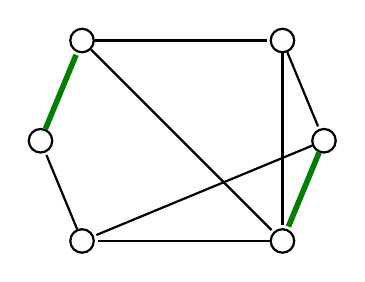
\begin{tikzpicture}[-,>=stealth,shorten >=1pt,auto,node distance=2cm, thick,main node/.style={scale=0.9,circle,draw,font=\sffamily\normalsize}]

            \node[] (x) []{};
            \node[main node] (1)[above left of = x] {};
            \node[main node] (2)[above right of = x] {};
            \node[main node] (3)[right of = x] {};
            \node[main node] (4)[below right of = x] {};
            \node[main node] (5)[below left of = x] {};
            \node[main node] (6)[left of = x] {};

            \path[every node/.style={font=\sffamily\small}]
                (1) edge (2)
                (2) edge (3)
                (3) edge[color = Green, line width = 2] (4)
                (4) edge (5)
                (5) edge (6)
                (6) edge[color = Green, line width = 2] (1)
                (1) edge (4)
                (2) edge (4)
                (3) edge (5)
                ;
        \end{tikzpicture}
        \caption{The green edges form a matching of the graph.}
    \end{figure}
    
    We're often interested in finding the matching with maximum cardinality. Before proceeding, it's important to distinguish between the concepts of \textbf{maximal} and \textbf{maximum}. In general, given a property $P$, a sub-structure $X$ of a structure $S$ is said to be maximal for $P$ over $S$ if $P(X)$ is true and there is no other sub-structure $X'$ of $S$ such that $P(X')$ is true and $X$ is contained inside $X'$. Instead, $X$ is said to be the maximum for $P$ over $S$ if $P(X)$ is true and there is no other sub-structure $X'$ of $S$ with a higher value for the property $P(X)$. For instance, the matching shown in the above figure is maximal because it cannot be extended with other edges without breaking the matching property, but it's not a maximum matching.

    \begin{figure}[H]
        \centering

        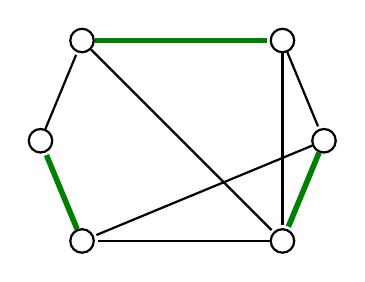
\begin{tikzpicture}[-,>=stealth,shorten >=1pt,auto,node distance=2cm, thick,main node/.style={scale=0.9,circle,draw,font=\sffamily\normalsize}]

            \node[] (x) []{};
            \node[main node] (1)[above left of = x] {};
            \node[main node] (2)[above right of = x] {};
            \node[main node] (3)[right of = x] {};
            \node[main node] (4)[below right of = x] {};
            \node[main node] (5)[below left of = x] {};
            \node[main node] (6)[left of = x] {};

            \path[every node/.style={font=\sffamily\small}]
                (1) edge[color = Green, line width = 2] (2)
                (2) edge (3)
                (3) edge[color = Green, line width = 2] (4)
                (4) edge (5)
                (5) edge[color = Green, line width = 2] (6)
                (6) edge (1)
                (1) edge (4)
                (2) edge (4)
                (3) edge (5)
                ;
        \end{tikzpicture}
        \caption{Maximum matching for the previous graph.}
    \end{figure}

    In particular, we'll focus on matching on \textbf{bipartite graphs}. These types of matchings are of particular interest due to how they describe many real-life situations. For instance, the problem of finding the optimal assignment of tasks to a group of employees can be solved by finding a maximum matching: we split the graph in two partitions, one with all the tasks and one with all the employees, connecting each employee to the tasks that he's capable of completing.

    \begin{figure}[H]
        \centering
        \resizebox{0.16\textwidth}{!}{
            \begin{tikzpicture}[-,>=stealth,shorten >=1pt,auto,node distance=2cm,thick,main node/.style={scale=1,circle,draw,font=\sffamily\normalsize}, rotate=90,transform shape]
                \node[main node] (1) [fill = Carmine,]{};
                \node[main node] (2) [fill = Carmine,right of=1] {};
                \node[main node] (3) [fill = Carmine,right of=2] {};
                \node[main node] (4) [fill = Carmine,right of=3] {};
                \node (5) [below right of=1] {};
                \node[main node] (6) [fill = BlueLagoon,below left of=5] {};
                \node[main node] (7) [fill = BlueLagoon,right of=6] {};
                \node[main node] (8) [fill = BlueLagoon,right of=7] {};
                \node[main node] (9) [fill = BlueLagoon,right of=8] {};

                \path[every node/.style={font=\sffamily\small}]
                        (1) edge (6)
                        (1) edge[color = Green, line width = 2] (9)
                        (2) edge (8)
                        (3) edge[color = Green, line width = 2] (6)
                        (3) edge (7)
                        (4) edge (8)
                        (4) edge (9)
                    ;
            \end{tikzpicture}
        }

        \caption{A matching on a bipartite graph.}
    \end{figure}

    Consider the matching on the bipartite graph shown above. We observe that this matching is neither maximal nor maximum. When the matching is not maximal, we can obtain a matching with greater cardinality simply by extending it.

    \begin{figure}[H]
        \centering
        \resizebox{0.16\textwidth}{!}{
                \begin{tikzpicture}[-,>=stealth,shorten >=1pt,auto,node distance=2cm,thick,main node/.style={scale=1,circle,draw,font=\sffamily\normalsize}, rotate=90,transform shape]
                \node[main node] (1) [fill = Carmine,]{};
                \node[main node] (2) [fill = Carmine,right of=1] {};
                \node[main node] (3) [fill = Carmine,right of=2] {};
                \node[main node] (4) [fill = Carmine,right of=3] {};
                \node (5) [below right of=1] {};
                \node[main node] (6) [fill = BlueLagoon,below left of=5] {};
                \node[main node] (7) [fill = BlueLagoon,right of=6] {};
                \node[main node] (8) [fill = BlueLagoon,right of=7] {};
                \node[main node] (9) [fill = BlueLagoon,right of=8] {};

                \path[every node/.style={font=\sffamily\small}]
                        (1) edge (6)
                        (1) edge[color = Green, line width = 2] (9)
                        (2) edge (8)
                        (3) edge[color = Green, line width = 2] (6)
                        (3) edge (7)
                        (4) edge[color = Green, line width = 2] (8)
                        (4) edge (9)
                    ;
            \end{tikzpicture}
        }

        \caption{A maximal matching on a bipartite graph.}
    \end{figure}

    We notice that the above matching is maximal, but not maximum. For instance, we observe that the number of edges outside of the matching that we selected form new matching with more edges than the one that we have considered. Hence, by \textit{swapping} all the edges, we get a matching with higher cardinality. Moreover, this new matching is clearly a maximum one since the number of nodes is equal to twice the number of selected edges.

    \begin{figure}[H]
        \centering
        \resizebox{0.16\textwidth}{!}{
            \begin{tikzpicture}[-,>=stealth,shorten >=1pt,auto,node distance=2cm,thick,main node/.style={scale=1,circle,draw,font=\sffamily\normalsize}, rotate=90,transform shape]
                \node[main node] (1) [fill = Carmine,]{};
                \node[main node] (2) [fill = Carmine,right of=1] {};
                \node[main node] (3) [fill = Carmine,right of=2] {};
                \node[main node] (4) [fill = Carmine,right of=3] {};
                \node (5) [below right of=1] {};
                \node[main node] (6) [fill = BlueLagoon,below left of=5] {};
                \node[main node] (7) [fill = BlueLagoon,right of=6] {};
                \node[main node] (8) [fill = BlueLagoon,right of=7] {};
                \node[main node] (9) [fill = BlueLagoon,right of=8] {};

                \path[every node/.style={font=\sffamily\small}]
                        (1) edge[color = Green, line width = 2] (6)
                        (1) edge (9)
                        (2) edge[color = Green, line width = 2] (8)
                        (3) edge (6)
                        (3) edge[color = Green, line width = 2] (7)
                        (4) edge (8)
                        (4) edge[color = Green, line width = 2] (9)
                    ;
            \end{tikzpicture}
        }

        \caption{The maximum matching obtained by swapping all the edges.}
    \end{figure}

    Let's take a closer look to what we just did. We notice that all the edges of the last non-maximum matching actually form a path whose edges alternate between being outside of the matching and inside of the matching. Moreover, both the first and last edge of such path are outside of the matching, hence the number of outside edges is one more than the number of inside edges. We generalize such paths through the concept of \textit{alternating path} and \textit{augmenting path}.
    
    \begin{frameddefn}{Alternating and augmenting path}
        Let $G$ be a bipartite graph and let $M \subseteq E(G)$ be a matching on $G$. An \textbf{$M$-alternating path} is a path starting from an unmatched node and whose edges alternate between $M$ and $E(G)-M$. If the path also ends at an unmatched node, the path is said to be \textbf{$M$-augmenting}.
    \end{frameddefn}

    To clarify this definition, let's make things more formal. A path $P = x_0 e_1 x_1 e_2 \ldots e_k x_k$ is $M$-alternating when $x_0$ is unmatched, meaning that there is no edge $e \in M$ in the matching such that $x_0 \in e$, and whose edges alternate between being outside of the matching and inside of the matching, meaning that $e_1 \notin M, e_2 \in M, e_3 \notin M$ and so on. When $x_k$ is also unmatched, the path is said to be $M$-augmenting. This name comes from the fact that, in order for $x_k$ to be unmatched, the last edge is not inside the matching, meaning that we have more edges outside of the matching then inside of it. Moreover, since $x_0$ and $x_k$ are unmatched, by swapping the edges inside of the matching with the edges outside of it we're guaranteed to get a matching (with more edges than the previous one).

    \begin{figure}[H]
        \centering
        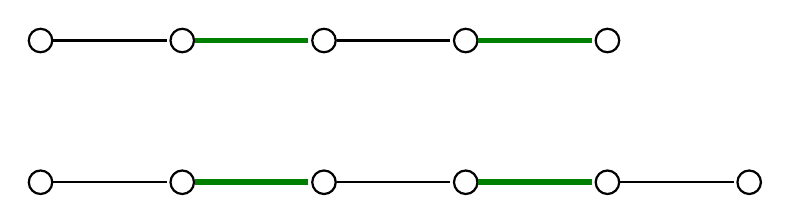
\begin{tikzpicture}[-,>=stealth,shorten >=1pt,auto,node distance=2cm,thick,main node/.style={scale=0.9,circle,draw,font=\sffamily\normalsize}]
            \node[main node] (1) []{};
            \node[main node] (2) [right of = 1]{};
            \node[main node] (3) [right of = 2]{};
            \node[main node] (4) [right of = 3]{};
            \node[main node] (5) [right of = 4]{};

            \node[main node] (6) [below of = 1]{};
            \node[main node] (7) [right of = 6]{};
            \node[main node] (8) [right of = 7]{};
            \node[main node] (9) [right of = 8]{};
            \node[main node] (10) [right of = 9]{};
            \node[main node] (11) [right of = 10]{};

            \path[every node/.style={font=\sffamily\small}]
                (1) edge (2)
                (2) edge[color = Green, line width = 2] (3)
                (3) edge (4)
                (4) edge[color = Green, line width = 2] (5)

                (6) edge (7)
                (7) edge[color = Green, line width = 2] (8)
                (8) edge (9)
                (9) edge[color = Green, line width = 2] (10)
                (10) edge (11)
            ;
        \end{tikzpicture}

        \caption{An $M$-alternating path (above) and an $M$-augmenting path (below).}
    \end{figure}

    \begin{framedlem}{}
        Let $G$ be a bipartite graph and let $M \subseteq E(G)$ be a matching on $G$. If $P$ is an $M$-augmenting path then $M \Delta E(P)$ is matching on $G$ with more edges than $M$
    \end{framedlem}

    \begin{proof}
        First, we recall that the \textit{symmetric difference} $M \Delta E(P)$ is defined as follows:
        \[M \Delta E(P) = (M \cup E(P)) - (M \cap E(P))\]

        Let $M' = M \Delta E(P)$. We observe that all the edges that aren't shared by $M$ and $P$ are also not in $M'$, hence we can ignore them. Let $P = x_0 e_1 x_1 e_2 \ldots e_k x_k$. Since $P$ is augmenting, the number of edges in $P$ that are also in $M$ is less than the number of edges that aren't in $M$. Hence, we get that $\abs{M'} > \abs{M}$.
    \end{proof}

    The above lemme gives us an easy way to increase the cardinality of our matching by finding augmenting paths and swapping edges. But how can we be sure that we have reached the maximum matching? \textcite{berge} proved that the above lemma can indeed be extended: if there are no augmenting paths then the matching is maximum.

    \begin{framedthm}[label={berge}]{Berge's theorem}
        Let $G$ be a bipartite graph and let $M \subseteq E(G)$ be a matching on $G$. Then, $M$ is a maximum matching on $G$ if and only if there are no $M$-augmenting paths.
    \end{framedthm}

    \begin{proof}
        One of the two implications directly follows from the previous lemma. For the other implication, we prove the contrapositive. Suppose that $M$ is a non-maximum matching on $G$. Then, there is at least one matching $M'$ on $G$ such that $\abs{M'} > \abs{M}$. Let $H \subseteq G$ be the graph such that $V(H) = V(G)$ and $E(H) = M \Delta M'$, where $\Delta$ denotes the \textit{symmetric difference}. We observe that every edge that is shared among $M$ and $M'$ gets deleted in $H$, hence we can ignore them.

        \textbf{Claim:} for every $x \in V(H)$ it holds that $\deg_H(x) \leq 2$.

        \begin{proof}[Proof of Claim 1.]
            Since $M$ and $M'$ are both matchings on $G$, each vertex can have at most one edge in $M$ and at most one edge in $M'$. If they share the same edge then $H$ won't contain such edge. If they don't, $x$ will have degree 2 in $H$.
        \end{proof}

        We observe that the above claim has many consequences. In particular, it implies that every component of $H$ must be either a cycle or a path (including trivial paths of one single vertex).
        
        \textbf{Claim 2}: every cycle component of $H$ has even length

        \begin{proof}[Proof of Claim 2.]
            By way of contradiction, suppose that there is a cycle $C$ of odd length. By construction, each component has to alternate between edges of $M$ and $M'$. Hence, at least one vertex of $C$ must have both edges lying either inside $M$ or $M'$, contradicting the fact that either $M$ or $M'$ is a matching. 
        \end{proof}

        Since $\abs{M'} > \abs{M}$, there must be a component with at least one (and at most one) edge in $M'$. Since the edges of each component alternate between $M$ and $M'$, by Claim 2 we know that such component cannot be a cycle. Hence, it must be a path component $P$. In order for $P$ to have more edges in $M'$ than edges in $M$, the first and last edge must be edges of $M'$, meaning that $P$ is an $M$-augmenting path. By contrapositive, if there is no $M$-augmenting path then $M$ is a maximum matching.
    \end{proof}

    This theorem has been used to construct many algorithms for finding a maximum matching on bipartite graphs. The most famous one is the \textbf{Hopcroft-Karp algorithm} \cite{hopcroft-karp}, due to a guaranteed runtime of $O(m \sqrt{n})$. Given a bipartite graph $G$ with bipartition $(A,B)$, the idea behind such algorithms is to run a simultaneous BFS starting from all the unmatched vertices of $A$, until at least
    one free node of $B$ is found. Then, we run a DFS over the forest produced by the BFS, starting from the unmatched nodes of $B$. Each path found through this procedure is an augmenting path, hence their edges can be swapped to increase the cardinality of the matching. The whole process is repeated until no augmenting path is found.

    What about non-bipartite graphs? For the general case, problems rise with odd cycles, which never exist in bipartite graphs (\Cref{bip_cycle}). Any matching over an odd-length cycle will never cover every vertex of the cycle. This means that in any odd-length cycle there must be a vertex adjacent to two edges which cannot be part of the matching considered. This makes finding the optimal matching hard to find on such graphs. In 1965, \textcite{blossom} came up with the \textbf{Blossom algorithm}, a real piece of art in the world of algorithm design. The algorithm is based on the repeated contraction and distension of \textit{blossoms}, i.e. a cycles of odd length which contain the maximal number of edges in the current matching. The \textit{blossom lemma} states that any matching found on the graph with every blossom contracted is a maximum matching if and only if it is also a maximum matching for the graph original graph.

    The maximum matching problem is highly related to the \textbf{Minimum Vertex Cover} problem. This problem involves finding the smallest subset of vertices in a graph such that every edge is incident to at least one vertex in the set.

    \begin{frameddefn}{Vertex Cover}
        Given a graph $G$, a vertex cover over $G$ is a subset $C \subseteq V(G)$ such that $\forall e \in E(G)$ there is a vertex $v \in C$ such that $v \in e$.
    \end{frameddefn}

    \begin{figure}[H]
        \centering
        \begin{tikzpicture}[-,>=stealth,shorten >=1pt,auto,node distance=1.75cm,thick,main node/.style={scale=0.9,circle,draw,font=\sffamily\normalsize}]
            \node[main node] (1) []{};
            \node[main node] (2) [fill = Carmine, below left of=1] {};
            \node[main node] (3) [fill = Carmine, below right of=1] {};
            \node[main node] (4) [fill = Carmine, below right of=2] {};
            \node[main node] (5) [below left of=2] {};
            \node[main node] (6) [below right of=3] {};

            \path[every node/.style={font=\sffamily\small}]
                (1) edge (2)
                (1) edge (3)
                (2) edge (4)
                (3) edge (4)
                (2) edge (5)
                (3) edge (6)
                (5) edge (4)
                (6) edge (4)
                ;
        \end{tikzpicture}

        \caption{The red nodes are the smallest possible vertex cover of the graph.}
    \end{figure}

    \begin{framedprop}{}
        Given a graph $G$, for every matching $M$ on $G$ and every vertex cover $V$ of $G$ it holds that $\abs{M} \leq \abs{V}$.
    \end{framedprop}

    \begin{proof}
        By definition, we observe that if $V$ is a vertex cover for $G$ then it is also a vertex cover for any subgrpah $G' \subseteq G$. Hence, $V$ is also a vertex cover for any $G_M$, where $V(G_M) = V(G)$ and $E(G_M) = M$. By definition of matching, in $G_M$ any vertex has either degree 0 or 1. Thus, each vertex of $V$ can cover at most one edge of $M$, meaning that $V$ has to have at least $\abs{M}$ vertices to cover all the edges of $M$.
    \end{proof}

    In bipartite graphs, the above proposition can be strengthened. In 1931, Kőnig \cite{konig} proved that the cardinality of the maximum matching and the minimum vertex cover is equal. This implies that the minimum vertex cover can be efficiently found on bipartite graphs by finding the maximum matching.

    \begin{framedthm}[label={konig}]{Kőnig's theorem}
        Given a bipartite graph $G$, let $M^*$ and $V^*$ respectively be a maximum matching and a minimum vertex cover on $G$. Then, it holds that $\abs{M^*} = \abs{V^*}$. 
    \end{framedthm}

    \begin{proof}
        We observe that it suffices to show that there is a (non-minimum) vertex cover $V$ such that $\abs{V} = \mathcal{M^*}$ in order to get $\abs{M^*} \leq \abs{V^*} \leq \abs{V} = \abs{M^*}$. Let $(A,B)$ be the bipartition of $G$. We define $V$ as the set of vertices such that $\forall ab \in M$, with $a \in A$ and $b \in B$, if there is an alternating path starting from a vertex in $A$ and ending on $b$ then $b \in V$, otherwise $a \in \mathrm{U}$. Fix an edge $xy \in E(G)$ with $x \in A$ and $y \in B$.
        
        \textbf{Claim:} $V$ covers $xy$
        \begin{proof}
            Suppose that $xy \in M$ then we know that either $x$ or $y$ is in $V$ by definition of $\mathrm{U}$ itself, meaning that such edge is covered. Hence, we may assume that $xy \notin M$. We have two cases:
            \begin{itemize}
                \item $x$ is unmatched, meaning that $\nexists uv \in M$ such that $u = x$. Then, $y$ must be matched by $M^*$ to some $u \in A$, since otherwise $M^* \cup \{xy\}$ would be a matching greater than $M^*$. Hence, the edge $uy$ is an alternating path starting from $A$ and ending on $y$, meaning that $y \in V$.
                \item $x$ is matched, meaning that $\exists xv \in M$. Then, by definition of $V$, either $x$ or $v$ must lie inside $V$. If $x \in \mathrm{U}$ then $xy$ is trivially covered by $V$. If $v \in V$, instead, by definition of $V$ there must be an alternating path $P$ starting from $A$ and ending at $v$. This also implies that $P \cup vx \cup xy$ is an alternating path ending on $y$. However, this implies that $y$ must be matched through some edge $wy \in M$, with $w \neq x$, since otherwise the path $P \cup vx \cup xy$ would be an augmenting path, contradicting the fact that $M^*$ is maximum (\nameref{berge}). Thus, we conclude that $y \in V$ since $wy \in M$ and $P \cup vx \cup xy$ is an augmenting path that ends on $y$.
            \end{itemize}
        \end{proof}

        In both cases, we get that either $x$ or $y$ is inside $V$, concluding that $xy$ is covered by $\mathrm{U}$. Applying the same argument over all edges, we get that $V$ is a vertex cover.
    \end{proof}

    \section{Perfect matching}
    
    We'll now focus on a particular type of matching on graphs. First, we notice that for any matching $M$ on a graph $G$ (even when $G$ is non-bipartite) it must always hold that:
    \[\abs{M} \leq \frac{\abs{V(G)}}{2}\]

    When the inequality is satisfied at equality, the matching is said to be \textbf{perfect}.We observe that such condition is equivalent to saying that every vertex of the graph is covered by an edge. In fact, the concept of perfect matching can be, in some sense, viewed as the edge-version of a vertex cover, even though there is an additional constraint for the disjointness of the edges.

    \begin{figure}[H]
        \centering

        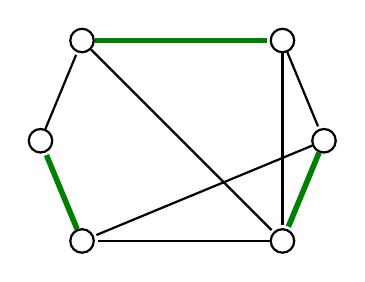
\begin{tikzpicture}[-,>=stealth,shorten >=1pt,auto,node distance=2cm, thick,main node/.style={scale=0.9,circle,draw,font=\sffamily\normalsize}]

            \node[] (x) []{};
            \node[main node] (1)[above left of = x] {};
            \node[main node] (2)[above right of = x] {};
            \node[main node] (3)[right of = x] {};
            \node[main node] (4)[below right of = x] {};
            \node[main node] (5)[below left of = x] {};
            \node[main node] (6)[left of = x] {};

            \path[every node/.style={font=\sffamily\small}]
                (1) edge[color = Green, line width = 2] (2)
                (2) edge (3)
                (3) edge[color = Green, line width = 2] (4)
                (4) edge (5)
                (5) edge[color = Green, line width = 2] (6)
                (6) edge (1)
                (1) edge (4)
                (2) edge (4)
                (3) edge (5)
                ;
        \end{tikzpicture}
        \caption{A perfect matching.}
    \end{figure}
    
    \begin{frameddefn}{Perfect matching}
        A matching $M$ on a graph $G$ is said to be perfect if for all vertices of $G$ there is an edge of $M$ covering it. 
    \end{frameddefn}

    We observe that every perfect matching is clearly a maximum one, but the contrary doesn't always hold. Moreover, not all graphs can have a perfect matching -- trivially, a graph with an isolated vertex cannot have a perfect matching.

    For bipartite graphs, the concept of perfect matching has to be slightly tweaked: if $(A,B)$ is the bipartition of the graph and $\abs{A} \neq \abs{B}$, there is no way for a perfect matching to hold. Hence, assuming that $\abs{A} \leq \abs{B}$, we use the concept of \textbf{$A$-perfect matching}, i.e. a matching that covers every vertex of $A$ -- notice that if $(A,B)$ is a partition then $(B,A)$ is also a partition, hence we can always assume that $\abs{A} \leq \abs{B}$.
    
    \textcite{hall} was able to characterize $A$-perfect matchings on bipartite graphs through the now now called \textit{Hall's Marriage Condition} -- the name comes from the original set-theoretic formulation of the problem.

    \begin{framedthm}[label={hall}]{Hall's marriage condition}
        Let $G$ be a bipartite graph with bipartition $(A,B)$ with $\abs{A} \leq \abs{B}$. Then, $G$ has an $A$-perfect matching if and only if for all subsets $S \subseteq A$ it holds that $\abs{N(S)} \geq \abs{S}$, where $N(S) = \bigcup_{s \in S} N(s)$.
    \end{framedthm}

    \begin{proof}
        Suppose that there is an $A$-perfect matching $M$ of $G$. Fix a subset $S \subseteq A$. By definition of $M$, each node $s \in S$ is matched through $M$ with a different node, therefore $\abs{N(S)} \geq \abs{S}$.

        Vice versa, suppose that there is no $A$-perfect matching $M$. Let $V^*$ be a minimum vertex cover on $G$. By \nameref{konig}, we know that the size of $V^*$ has to be equal to the size of any maximum matching of $G$. However, since there is no $A$-perfect matching, any maximum matching has to have size less than $\abs{A}$, meaning that $\abs{V^*} < \abs{A}$. Consider now the set $S = A-V^*$. Since $G$ is bipartite, it must hold that $N(S) = V^* \cap B$. We observe that:
        \[\abs{N(S)} \leq \abs{V^* \cap B} = \abs{V^*} - \abs{V^* \cap A}\]

        Since $V^* \cap A = A - (A - V^*) = A - S$, we get that:
        \[\abs{N(S)} \leq \abs{V^*} - \abs{V^* \cap A} = \abs{V^*} - \abs{A} + \abs{S}\]

        Finally, since $\abs{U} < \abs{A}$, we conclude that:
        \[\abs{N(S)} \leq \abs{V^*} - \abs{V^* \cap A} = \abs{V^*} - \abs{A} + \abs{S} < \abs{S}\]
    \end{proof}

    What if the graph is non-bipartite? Can perfect matchings also be characterized for the general case? The answer is yes! Before proving the result, we'll build an intuition for it. First, we observe that each graph with an odd number of vertices cannot have a perfect matching since there will always be at least one unmatched vertex. This can be extended to components: if a graph contains at least one component with an odd number of vertices then there will always be at least one unmatched vertex inside that component. But what if such components get \curlyquotes{connected} through an intermediate vertex $x$? Then, once such vertex gets matched, the problem still holds: the induced graph $G-x = G[V(G)-\{x\}]$ now contains components with an odd number of vertices.

    \begin{figure}[H]
        \centering
        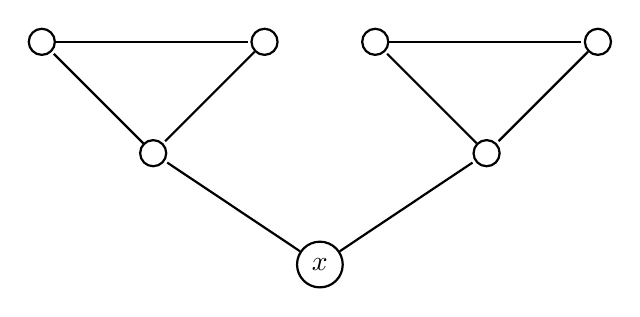
\begin{tikzpicture}[-,>=stealth,shorten >=1pt,auto,node distance=2cm,thick,main node/.style={scale=1,circle,draw,font=\sffamily\normalsize}]
            \node[main node] (1) []{$x$};

            \node[main node] (2) [above left of = 1, xshift=-20]{};
            \node[main node] (3) [above left of = 2]{};
            \node[main node] (4) [above right of = 2]{};

            \node[main node] (5) [above right of = 1, xshift=20]{};
            \node[main node] (6) [above left of = 5]{};
            \node[main node] (7) [above right of = 5]{};

            \path[every node/.style={font=\sffamily\small}]
                (1) edge (2)
                (1) edge (5)

                (2) edge (3)
                (3) edge (4)
                (4) edge (2)
                
                (5) edge (6)
                (6) edge (7)
                (7) edge (5)
            ;
            \end{tikzpicture}

        \caption{Once the vertex $x$ gets matched, the graph $G-\{x\}$ is made of two odd components, making a perfect matching impossible.}
    \end{figure}
    
    But what if we add another edge? In that case, we would have enough vertices to complete the perfect matching. 

    \begin{figure}[H]
        \centering
        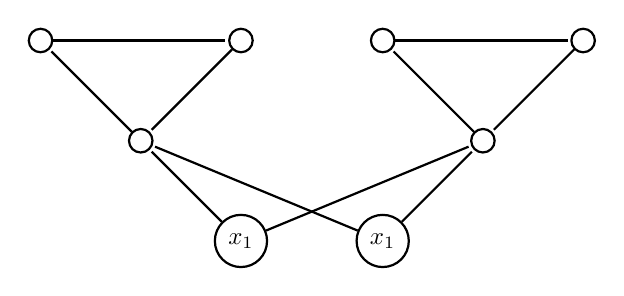
\begin{tikzpicture}[-,>=stealth,shorten >=1pt,auto,node distance=2cm,thick,main node/.style={scale=0.9,circle,draw,font=\sffamily\normalsize}]
            \node[main node] (1) []{$x_1$};
            \node[main node] (8) [right of = 1]{$x_1$};

            \node[main node] (2) [above left of = 1]{};
            \node[main node] (3) [above left of = 2]{};
            \node[main node] (4) [above right of = 2]{};

            \node[main node] (5) [above right of = 8]{};
            \node[main node] (6) [above left of = 5]{};
            \node[main node] (7) [above right of = 5]{};

            \path[every node/.style={font=\sffamily\small}]
                (1) edge (2)
                (1) edge (5)
                (8) edge (2)
                (8) edge (5)

                (2) edge (3)
                (3) edge (4)
                (4) edge (2)
                
                (5) edge (6)
                (6) edge (7)
                (7) edge (5)
            ;
            \end{tikzpicture}

        \caption{Once the vertex $x_1$ gets matched with an edge touching one of the two odd components, $x_2$ can be matched through the edges touching the other component.}
    \end{figure}

    Thus, it's easy to see that if there is a subset of vertices $S \subseteq V(G)$ such that $\mathcal{O}(G-S) > \abs{S}$ then there cannot be a perfect matching, where $\mathcal{O}(G)$ is the number of odd components of $G$. To make things easier to read, we say that a graph satisfies the \textbf{perfect matching condition} when for all subsets $S \subseteq V(G)$ it holds that $\mathcal{O}(G-S) \leq \abs{S}$. In 1947, Tutte \cite{tutte} proved that such condition perfectly characterizes the existence of a perfect matching. To show the result, we first prove the following lemma.

    \begin{framedlem}{}
        Let $G$ be a graph and let $G'$ be a super-graph of $G$, i.e. $G \subseteq G'$, obtained by adding edges to $G$ and keeping the same vertices. Then, if $G'$ doesn't satisfy the perfect matching condition then $G$ also doesn't.
    \end{framedlem}

    \begin{proof}
        Suppose that $G'$ doesn't satisfy the condition, meaning that $\exists S \subseteq V(G)$ such that $\mathcal{O}(G'-S) > \abs{S}$. Then, since $G'$ is obtained by adding edges, the number of odd components in $G'$ may remain the same of $G$ or decrease if two previously disconnected components are now connected in $G'$, meaning that:
        \[\abs{S} < \mathcal{O}(G'-S) \leq \mathcal{O}(G-S)\]
        and thus that $G$ also doesn't satisfy the condition.
    \end{proof}

    \begin{framedthm}{Tutte's theorem}
        Let $G$ be a graph. Then, $G$ has a perfect matching if and only if for all subsets $S \subseteq V(G)$ it holds that $\mathcal{O}(G-S) \leq \abs{S}$.
    \end{framedthm}
    
    \begin{proof}
        Suppose that there is a perfect matching $M$ on $G$. Fix a subset $S \subseteq V(G)$. Then, every odd component of $G-S$ sends at least one matching edge to a distinct vertex of $S$, meaning that $\abs{S} \geq \mathcal{O}(G-S)$.

        Vice versa, suppose that there is no perfect matching on $G$. Let $G'$ be the maximal super-graph of $G$ that doesn't have a perfect matching obtained by adding edges and keeping the same vertices. We say that a set $X$ satisfies the \textit{clique-adjacency condition} if every component of $G'[V(G')-X]$ is a clique and every $u \in X$ is adjacent to every $v \notin X$

        \textbf{Claim 1:} if there is a subset $S' \subseteq V(G')$ that satisfies the clique-adjacency condition then $G$ doesn't satisfy the perfect matching condition.

        \begin{proof}[Proof of Claim 1.]
            Assume that $S'$ is a subset satisfying the clique-adjacency condition. We observe that, since very component of $G'[(V(G))-S']$ is a clique, for each even component we can always find a perfect matching restricted to it. For odd components, instead, we can always find a perfect matching over all its nodes except for one. Let $M_1, \ldots, M_k$ be the perfect matching defined on the even components and let $M'_1, \ldots, M'_h$ be the p.m. defined on the odd components.

            If $S'$ violates the perfect matching condition on $G$ then we're done. Otherwise, if $S'$ doesn't violate it then we know that $\abs{S'} \geq \mathcal{O}(G-S')$. Hence, since every vertex of $S'$ is adjacent to every vertex that isn't in $S'$, we can match the unmatched vertex of each odd component of $G'[V(G)-S']$ with a vertex of $S'$. We observe that the remaining vertices of $S'$ must form a clique, since otherwise we could add edges to $G'$ and preserve the absence of a perfect matching (the only way to prevent this is if all the edges are already in the graph). Moreover, this clique must have an odd number of nodes, since otherwise we could form a perfect matching on $G'$. Hence, $G'$ must have an odd number of total vertices (thus also $G$ does), meaning that the empty set $\varnothing$ violates the perfect matching condition on $G$. Hence, at least one subset of $G$ must violate the perfect matching condition.
        \end{proof}

        Let $S = \{v \in V(G') \mid \deg_{G'}(v) = n-1\}$. By way of contradiction, suppose that that $S$ doesn't satisfy the clique-adjacency condition. Then, there is a component of $G'[V(G')-X]$ that isn't a clique or there is a $u \in S$ and a $v \notin S$ such that $u \not\sim v$. However, by definition of $S$, the second case cannot hold, hence there must be a component that isn't a clique, meaning that there are at least two vertices $x,y$ in that component such that $x \not\sim y$. 

        Let $P$ be the shortest path from $x$ to $y$ in $G'[V(G')-S]$. Let $a,b,c$ be the first vertices of $P$. We observe that $a \not\sim c$ since otherwise $P$ wouldn't be the shortest path. Moreover, since $P$ is a path in $G'[V(G')-S]$, we know that $b \notin S$. Hence, there must be a vertex $d \in V(G)$ such that $b \not\sim d$. In other words, we obtain a kite-shaped subgraph (see \Cref{kite_tutte}).

        By maximality of $G'$, we know that $G' \cup \{ac\}$ must have a perfect matching $M_1$. Likewise, $G' \cup \{bd\}$ must have a perfect matching $M_2$. Furthermore, it must hold that $ac \in M_1$ and $bd \in M_2$ since otherwise $M_1$ and $M_2$ would be perfect matchings on $G'$. 

        \textbf{Claim 2}: $(M_1 - \{ac\}) \cup (M_2 - \{bd\})$ contains a perfect matching on $G'$

        \begin{proof}[Proof of Claim 2.]
            Let $\overline{M} = (M_1 - \{ac\}) \Delta (M_2 - \{bd\})$. Since $M_1$ and $M_2$ are two matchings, every vertex of $\overline{M}$ has degree at most 2. Hence, every component of $\overline{M}$ must be either an alternating path or an alternating cycle. Moreover, we observe that the only vertices that have degree 1 are $a,b,c,d$. Thus, these vertices must be the endpoints of two components $P_1, P_2$ that are alternating paths. We observe that, since $ac \in M_1$ and $bd \in M_2$, one of such paths must be an $M_1$-alternating path, while the other must be an $M_2$-alternating path. Without loss of generality, let $P_1$ be the $M_1$-alternating path and let $P_2$ be the $M_2$-alternating path. We notice that $M' = (M_1 \cup M_2) - (E(P_1) \cup E(P_2))$ is a perfect matching on $G - (V(P_1) \cup V(P_1))$. We have three cases:
            \begin{enumerate}
                \item $P_1$ is a path from $a$ to $c$ and $P_2$ is a path from $b$ to $d$. Then, $(M_1 \cap E(P_2)) \cup (M_2 \cap E(P_1)) \cup M'$ is a perfect matching on $G'$ 
                \item $P_1$ is a path from $a$ to $b$ and $P_2$ is a path from $c$ to $d$. Then, $(M_1 \cap E(P_2)) \cup (M_2 \cap E(P_1)) \cup M' \cup \{bd\}$ is a perfect matching on $G'$ 
                \item $P_1$ is a path from $a$ to $d$ and $P_2$ is a path from $b$ to $d$. Then, $(M_1 \cap E(P_2)) \cup (M_2 \cap E(P_1)) \cup M' \cup \{ac\}$ is a perfect matching on $G'$ 
            \end{enumerate}
        \end{proof}

        Since $(M_1 - \{ac\}) \cup (M_2 - \{bd\})$ always contains a perfect matching on $G'$, we conclude that $S$ it is impossible for $S$ to not satisfy the clique-adjacency condition. Thus, through Claim 1 and the previous lemma we know that both $G'$ and $G$ violate the perfect matching condition.
    \end{proof}

    \begin{figure}[H]
        \centering
        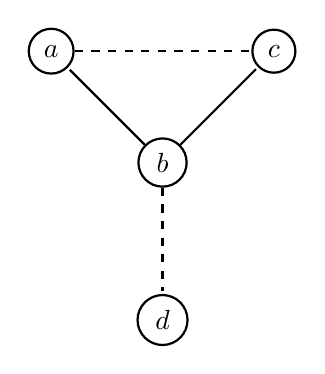
\begin{tikzpicture}[-,>=stealth,shorten >=1pt,auto,node distance=2cm,thick,main node/.style={scale=1,circle,draw,font=\sffamily\normalsize}]
            \node[main node] (1) []{$b$};
            \node[main node] (2) [above left of = 1]{$a$};
            \node[main node] (3) [above right of = 1]{$c$};
            \node[main node] (4) [below of = 1]{$d$};

            \path[every node/.style={font=\sffamily\small}]
                (1) edge (2)
                (1) edge (3)
                (1) edge[dashed] (4)
                (2) edge[dashed] (3)
            ;
            \end{tikzpicture}

        \caption{The kite-shaped subgraph yield by Tutte's argument. The dashed edges represent non-existing edges.}
        \label{kite_tutte}
    \end{figure}

    \newpage

    \section{Stable matching}

    We'll now focus on a more advanced type of maximum, i.e. the \textbf{Stable Marriage} problem. This problem acts as a generalization of the common maximum matching problem, where the entities involved can have some \textit{preferences} for their possible partners. In general, a matching on a bipartite graph is said to be \textbf{stable} if no vertex is unmatched and there is no other possible partner outside of the matching that they would prefer to be matched with. The preferences of each vertex $v \in V(G)$ are described through a bijective weight function $w_v : V \to [\abs{X}]$, where $X = B$ if $v \in A$ and $X = A$ otherwise.

    \begin{frameddefn}{Stable matching}
        Let $G$ be a bipartite graph and let $\{w_v\}_{v \in V(G)}$ be a family of preference functions. A matching $M$ on $G$ is said to be \textbf{stable} if for all edges $ab \in E(G)$ at least one of the following holds:
        \begin{itemize}
            \item $a$ is matched and $\nexists ab' \in M$ such that $w_a(b) > w_a(b')$
            \item $b$ is matched and $\nexists a'b \in M$ such that $w_b(a) > w_a(a')$
        \end{itemize}
    \end{frameddefn}

    \begin{figure}[H]
        \centering
        \resizebox{0.2\textwidth}{!}{
            \begin{tikzpicture}[-,>=stealth,shorten >=1pt,auto,node distance=2cm,thick,main node/.style={scale=1,circle,draw,font=\sffamily\normalsize}]
                \node[main node] (1) [fill = Carmine, text = white]{$a$};
                \node[main node] (2) [fill = Carmine, text = white,above of=1] {$b$};
                \node[main node] (3) [fill = Carmine, text = white,above of=2] {$c$};
                \node[main node] (4) [fill = Carmine, text = white,above of=3] {$d$};
                \node (5) [below right of=1] {};
                \node[main node] (6) [fill = BlueLagoon, text = white,above right of=5] {$1$};
                \node[main node] (7) [fill = BlueLagoon, text = white,above of=6] {$2$};
                \node[main node] (8) [fill = BlueLagoon, text = white,above of=7] {$3$};
                \node[main node] (9) [fill = BlueLagoon, text = white,above of=8] {$4$};

                \path[every node/.style={font=\sffamily\small}]
                        (1) edge[color = Green, line width = 2] (6)
                        (1) edge (9)
                        (2) edge[color = Green, line width = 2] (8)
                        (3) edge (6)
                        (3) edge[color = Green, line width = 2] (7)
                        (4) edge (8)
                        (4) edge[color = Green, line width = 2] (9)
                    ;
            \end{tikzpicture}
        }
        \[\begin{array}{ccc}
            w_a : 4231 & \qquad\qquad & w_1 : acbd \\
             w_b : 4123 & \qquad\qquad & w_2 : abdc \\
            w_c : 1243 & \qquad\qquad & w_3 : bcda \\
            w_d : 3241 & \qquad\qquad & w_4 : dcba \\
        \end{array}\]

        \caption{A stable matching. The preferences are represented through ordered lists}
    \end{figure}

    We observe that the definition of stable matching implies that the trivial empty matching is \underline{not stable}, since at least one of the two endpoints of every edge has to be matched. Surprisingly, \textcite{gale_shapley} proved that in any bipartite graphs it is always possible to find a stable matching independently of all preferences and entities involved. The result was first proved in the context of mathematical economics, solving the problem of optimal matching processes, such as college admission, job recruiting, hospital admitting and many more, awarding the two authors the \textit{2012 Nobel Prize in Economics}. Before proving the result, we give some a \curlyquotes{name} to some properties in order to make things more readable:
    \begin{itemize}
        \item Given two matchings $M,M'$ on a graph $G$, we say that $M'$ is \textbf{better} than $M$ if for all $ab \in M'$ there is at least an edge $a'b \in M$ such that $w_b(a') \geq w_b(a)$ and there is at least an edge $a''b \in M'$ such that $w_b(a) > w_b(a'')$. In other words, there is at least one edge that is strictly more preferable, while all the other edges are at least as good as the ones in $M$.
        
        \item We say that a vertex $a \in A$ is \textbf{acceptable} for $b \in B$ if either $b$ is unmatched or $b$ is matched to $a' \in A$ but $w_b(a) > w_b(a')$. In other words, $b$ is either unmatched or matched to a partner less preferred than $a$. 
        
        \item We say that $a \in A$ is \textbf{happy} if either $a$ is unmatched or $a$ is matched to $b \in B$ and for all $b' \in B$ that find $a$ acceptable it holds that $w_a(b) \geq w_a(b')$. In other words, $a$ is either unmatched or has reached its optimal partner.
    \end{itemize}

    \begin{framedthm}{Gale-Shapley theorem}
        Every bipartite graph with a family of preference functions $\{w_v\}_{v \in V(G)}$ has a stable matching.
    \end{framedthm}

    \begin{proof}
        We give a constructive proof. The idea is to construct a sequence of matchings $M_0, \ldots, M_k$ such that for each matching it holds that every vertex of $A$ is happy inside it, but only the last matching is stable. First, we claim the following.

        \textbf{Claim 1}: if $M$ is not stable and every vertex of $A$ is happy in $M$ then there is no $a \in A$ such that $a$ is unmatched and acceptable for some $b \in B$

        \begin{proof}[Proof of Claim 1.]

            Suppose that $M$ is not stable and that every vertex of $A$ is happy in $M$. Then, by definition of unstable matching, there must be at least one edge $ab \in E(G)$ for which one of the following four cases holds:
            \begin{enumerate}
                \item $a$ is unmatched and $b$ is unmatched. Then, $a$ is acceptable for $b$ since the latter is unmatched.
                \item $a$ is unmatched and $\exists a'b \in M$ such that $w_b(a) > w_b(a')$. Then, $a$ is acceptable for $b$ since the latter is matched to $a'$ but $a$ is a more preferred partner for $b$.
                \item $\exists ab' \in M$ such that $w_a(b) > w_a(b')$ and $b$ is unmatched. Then, $a$ is acceptable to $b$ since the latter is unmatched, contradicting the fact that $a$ is happy in $M$ since $a$ is matched to $b'$ but prefers $b$.
                \item $\exists ab' \in M$ such that $w_a(b) > w_a(b')$ and $\exists a'b \in M$ such that $w_b(a) > w_b(a')$. Then, $a$ is acceptable to $b$ since $a$ is a more preferred partner for $b$, contradicting the fact that $a$ is happy in $M$ since $a$ is matched to $b'$ but prefers $b$.
            \end{enumerate}

            Hence, the only possibilities are the first and second case, concluding that $a$ is unmatched and acceptable for $b$.
        \end{proof}
        
        We'll now define the extension procedure. Let $M_0 = \varnothing$. Since the matching is empty, each vertex of $A$ is unmatched, hence happy. Moreover, by definition $M_0$ cannot be stable. This will act as our base case. Fix $i \in [k]$ and suppose that $M_i$ is unstable and every vertex inside it is happy. Then, by Claim 1 there must be a vertex $a_{i+1} \in A$ that is unmatched in $M_i$ and must have at least one $b \in B$ that finds $a$ acceptable. Let $b_{i+1}$ be a vertex of $B$ that finds $a$ acceptable and that maximizes the value of $w_{a+1}(b_{i+1})$. We set $M_{i+1}$ as the matching obtained by removing the potential already existing partner $a'$ of $b_{i+1}$ in $M_i$ and by adding the edge $a_{i+1}b_{i+1}$
        \[M_{i+1} = \soe{ll}{
            M_i \cup \{a_{i+1} b_{i+1}\} & \text{if } \nexists a'b_{i+1} \in M_i\\
            (M_i \cup \{a_{i+1} b_{i+1}\}) - \{a'b_{i+1}\} & \text{otherwise}
        }\]

        We claim that the extended matching is better than the previous and preserves happiness for all vertices.

        \textbf{Claim 2}: $M_{i+1}$ is better than $M_i$ and every vertex of $A$ is happy in $M_{i+1}$.

        \begin{proof}[Proof of Claim 2.]
            By construction, every edge $xy \in M_i$ such that $y \neq b_{i+1}$ is also inside $M_{i+1}$, hence every such edge preserves happiness and the overall preferences of each vertex. If $\nexists a'b_{i+1} \in M_i$ then $M_{i+1}$ is trivially better than $M_{i}$. If $\exists a'b_{i+1} \in M_i$, instead, the new edge $a_{i+1}b_{i+1}$ since $a_{i+1}$ is acceptable for $b$, meaning that $M_{i+1}$ is better than $M_i$ also in this case. Moreover, by choice of $b_{i+1}$, the vertex $a_{i+1}$ is now matched with an optimal partner. Hence, the happiness of $a_{i+1}$ is preserved: $a_{i+1}$ was happy due to it being unmatched, but now it's happy due to being matched with the best partner. Moreover, the happiness of the potential vertex $a'$ is also happy since it became unmatched.
        \end{proof}

        Since every matching in the sequence is better than the previous ones, we know that such sequence cannot cycle. Moreover, since there is a finite number of possible matchings, the sequence will eventually reach a matching where every vertex of $A$ is matched. Let $M_k$ be such matching. Then, by contrapositive of Claim 1, we know that $M_k$ is either stable or has a vertex that isn't happy. However, by construction of the sequence, we know that every vertex in $M_k$ is happy, thus the only possibility is that $M_k$ is stable.
    \end{proof}

    \newpage

    \section{Solved exercises}

    \begin{framedprob}{}
        Let $G$ be a bipartite $k$-regular graph with bipartition $(A,B)$. Prove that:
        \begin{enumerate}
            \item $\abs{A} = \abs{B}$
            \item $G$ has a perfect matching
        \end{enumerate} 
    \end{framedprob}

    \begin{proof}[Solution]
        Given any set $X$, let $E_X$ denote the subset of edges with an endpoint in $X$. Since the graph is $k$-regular, we have that $\abs{E_A} = k \abs{A}$ and $\abs{E_B} = k\abs{B}$. Moreover, since the graph is bipartite, we have that $E_A = E_B$. Hence, we get that $k \abs{A} = k \abs{B}$ and thus that $\abs{A} = \abs{B}$. Consider now a subset $S \subseteq A$. We observe that $E_S \subseteq E_{N(S)}$ by definition of neighborhood. Hence, we have that $k \abs{S} = \abs{E_S} \leq \abs{E_{N(S)}} = k \abs{N(S)}$ and thus that $\abs{S} \leq \abs{N(S)}$. By \nameref{hall}, we conclude that $G$ has a perfect matching.
    \end{proof}

    \chapter{Connectivity and Structure}

    \section{Disjoint paths, hitting set and separations}

    Many tools of graph theory enable us to study the structure of the underlying graph when some conditions are met. One such tool is \textbf{Menger's theorem}, which can be used to derive many results regarding the structure of graphs. We'll start by defining the tools needed to discuss such theorem.

    \begin{frameddefn}{$(A,B)$ path}
        Let $G$ be a graph. Given two subsets $A,B \subseteq V(G)$, an $(A,B)$ path is a path with one endpoint in $A$, one endpoint in $B$ and no internal vertices in $A \cup B$
    \end{frameddefn}

    \begin{figure}[H]
        \centering
        \resizebox{0.3 \textwidth}{!}{
            \begin{tikzpicture}[-,>=stealth,shorten >=1pt,auto,node distance=2cm,thick,main node/.style={scale=1,circle,draw,font=\sffamily\normalsize}]
                \node[main node] (1)[fill = Carmine, text = white]{};
                \node[main node] (2)[above of = 1]{};
                \node[main node] (3)[fill = Carmine, text = white, below of = 1]{};
                \node[main node] (4)[fill = Carmine, text = white, below of = 3]{};

                \node[main node] (5)[right of = 1]{};
                \node[main node] (6)[right of = 3]{};
                \node[main node] (7)[right of = 5]{};
                \node[main node] (8)[right of = 6]{};

                \node[main node] (10)[fill = BlueLagoon, text = white, right of = 7]{};
                \node[main node] (9)[above of = 10]{};
                \node[main node] (11)[fill = BlueLagoon, text = white, below of = 10]{};
                \node[main node] (12)[below of = 11]{};

                \path[every node/.style={font=\sffamily\small}]
                    (1) edge[color = Green, line width = 2] (5)
                    (2) edge (5)
                    (3) edge (6)
                    (4) edge[color = Orange, line width = 2] (6)

                    (5) edge (6)
                    (5) edge[color = Green, line width = 2] (7)
                    (6) edge (7)
                    (6) edge[color = Orange, line width = 2] (8)

                    (7) edge (8)
                    (7) edge (9)
                    (7) edge[color = Green, line width = 2] (11)
                    (8) edge[color = Orange, line width = 2] (10)
                    (8) edge (12)
                ;
            \end{tikzpicture}
        }

        \caption{The blue nodes form the set $A$, while the red nodes form the set $B$. The colored paths form the maximum number of vertex-disjoint $(A,B)$ paths.}
        \label{hitting_set}
    \end{figure}

    We're interested in finding the maximum number of \textbf{vertex-disjoint $(A,B)$ paths}, i.e. paths that share no common edges. In many cases, we can identify a \curlyquotes{bottleneck} called \textbf{hitting set}, i.e. a set of vertices where all disjoint paths are forced to pass, such as the middle nodes of the graph in \Cref{hitting_set}.

    \begin{frameddefn}{$(A,B)$ Hitting set}
        Let $G$ be a graph. Given two subsets $A,B \subseteq V(G)$, an $(A,B)$ \textbf{hitting set} is a subset $X \subseteq V(G)$ such that every $(A,B)$ path intersects $X$. 
    \end{frameddefn}

    \begin{framedprop}{}
        Let $G$ be a graph and let $k \in \N$. Given two subsets $A,B \subseteq V(G)$, if there is an $(A,B)$ hitting set of size $k$ then there are at most $k$ vertex-disjoint $(A,B)$ paths.
    \end{framedprop}

    \begin{proof}
        Let $X$ be an $(A,B)$ hitting set of size $k$. By definition, every $(A,B)$ path must have at least one vertex in $H$. Hence, there can be at most $k$ vertex-disjoint $(A,B)$ paths.
    \end{proof}

    The above proposition clearly implies that the maximum number of disjoint $(A,B)$ paths is upper bounded by the cardinality of the minimum $(A,B)$ hitting set. However, finding hitting sets is no easy task. A more convenient way to reason about hitting sets are \textbf{graph separations}.

    \begin{frameddefn}{$(A,B)$ Separation}
        Let $G$ be a graph. Given two subsets $A,B \subseteq V(G)$, an $(A,B)$ \textbf{separation} is a pair of subsets $X,Y \subseteq V(G)$ for which all of the following conditions holds:
        \begin{enumerate}
            \item $A \subseteq X$ and $B \subseteq Y$
            \item $X \cup Y = V(G)$ 
            \item $\nexists uv \in E(G)$ such that $x \in X - Y$ and $y \in Y - X$
        \end{enumerate} 

        The \textbf{order} of an $(A,B)$ separation is defined as $\abs{X \cap Y}$.
    \end{frameddefn}

    \begin{figure}[H]
        \centering
        \resizebox{0.45 \textwidth}{!}{
            \begin{tikzpicture}[-,>=stealth,shorten >=1pt,auto,node distance=2cm,thick,main node/.style={scale=1,circle,draw,font=\sffamily\normalsize}]
                \node[main node] (1)[fill = Carmine, text = white]{};
                \node[main node] (2)[above of = 1]{};
                \node[main node] (3)[fill = Carmine, text = white, below of = 1]{};
                \node[main node] (4)[fill = Carmine, text = white, below of = 3]{};

                \node[main node] (5)[right of = 1]{};
                \node[main node] (6)[right of = 3]{};
                \node[main node] (7)[right of = 5]{};
                \node[main node] (8)[right of = 6]{};

                \node[main node] (10)[fill = BlueLagoon, text = white, right of = 7]{};
                \node[main node] (9)[above of = 10]{};
                \node[main node] (11)[fill = BlueLagoon, text = white, below of = 10]{};
                \node[main node] (12)[below of = 11]{};

                \draw (0.75,-1) ellipse (2 and 4);
                \draw (4.5,-1) ellipse (3.25 and 4);

                \path[every node/.style={font=\sffamily\small}]
                    (1) edge (5)
                    (2) edge (5)
                    (3) edge (6)
                    (4) edge (6)

                    (5) edge (6)
                    (5) edge (7)
                    (6) edge (7)
                    (6) edge (8)

                    (7) edge (8)
                    (7) edge (9)
                    (7) edge (11)
                    (8) edge (10)
                    (8) edge (12)
                ;
            \end{tikzpicture}
        }

        \caption{An $(A,B)$ separation of order 2.}
    \end{figure}

    From the very definition of separation, it's easy to see that every $(A,B)$ must pass through the intersection between $X$ and $Y$ since there are no edges that go from $X-Y$ to $Y-X$. Moreover, for any hitting set there is always a separation whose intersection is the hitting set itself, making the two concepts \curlyquotes{equivalent} for our purposes.

    \begin{framedprop}{}
        Let $G$ be a graph. Given two subsets $A,B \subseteq V(G)$, it holds that:
        \begin{itemize}
            \item If $X,Y$ form an $(A,B)$ separation then $X \cap Y$ is an $(A,B)$ hitting set.
            \item If $Z$ is an $(A,B)$ hitting set then there is an $(A,B)$ separation $P,Q$ such that $P \cap Q = Z$. 
        \end{itemize} 
    \end{framedprop}

    \begin{proof}
        The first point follows from the definition of $(A,B)$ separation. Suppose now that $Z$ is an hitting set. Let $H_1, \ldots ,H_t$ be the components of $G-Z$. We observe that no component has an edge $\{u,v\}$ such that $u \in A-Z$ and $v \in B-Z$, since otherwise there would be an $(A,B)$ path that doesn't intersect $Z$. Let $P,Q$ be the two subsets defined as:
        \[P = Z \cup \bigcup_{\substack{H_i \text{ s.t.}\\ A \cap H_i = \varnothing}} V(H)\]  
        \[Q = Z \cup \bigcup_{\substack{H_i \text{ s.t.}\\ A \cap H_i \neq \varnothing}} V(H)\]  

        By the above observation, $P$ contains all the vertices in $B-Z$, while $Q$ contains all the vertices in $V(G) - (B-Z)$, concluding that $P \cup Q = V(G)$ and $P \cap Q = Z$.
    \end{proof}

    The two previous propositions easily imply that the minimum order of an $(A,B)$ separation is equal to the minimum cardinality of an hitting set, implying that the former also gives an upper bound on the maximum number of vertex-disjoint $(A,B)$ paths. \textcite{menger} proved that the lower bound also holds, meaning that the two optimization problems are equivalent. To prove Menger's result, we'll prove a stronger version of the theorem.
    
    \begin{framedthm}[label={menger}]{Menger's theorem (stronger version)}
        Let $G$ be a graph and let $k \in \N$. Given two subsets $A,B \subseteq V(G)$, there are either at least $k$ vertex-disjoint $(A,B)$ paths or there is an $(A,B)$ separation of order less than $k$.
    \end{framedthm}

    \begin{proof}
        We proceed by induction of $\abs{E(G)}$. If $\abs{E(G)} = 0$ then the only possible $(A,B)$ paths are individual nodes in $A \cap B$. If $\abs{A \cap B} \geq k$ then we have at least $k$ vertex-disjoint $(A,B)$ paths. If $\abs{A \cap B} < k$, instead, $A \cap B$ is an hitting set, concluding by the previous proposition that there is an $(A,B)$ separation of order less then $k$.

        Assume that the lemma holds for every graph with at most $m-1$ edges. Suppose that $\abs{E(G)} = m$ and fix an edge $xy \in E(G)$. By inductive hypothesis, we know that $G-\{xy\}$ has either at least $k$ vertex-disjoint $(A,B)$ paths or there is an $(A,B)$ separation of order less than $k$. If the first case holds then $G$ also has at least $k$ vertex-disjoint $(A,B)$ paths, hence we may focus on the second case. Let $X,Y$ be an $(A,B)$ separation in $G-\{xy\}$ of order less than $k$. We observe that if $x,y \in X$ or $x,y \in Y$ then $X,Y$ is also a separation for $G$.
        
        Suppose now that $x \in X-Y$ and $y \in Y-X$. Then, $X$ and $Y\cup \{x\}$ is either still a separation of order less than $k$ or it becomes a separation of order $k$. Since the first case concludes the proof, we assume the second one to hold. Consider the graphs $G[X]$ and $G[Y]$. By inductive hypothesis, the former has either at least $k$ disjoint paths from $A$ to $(X \cap Y) \cup \{x\}$ or a separation of order less than $k$. Likewise, the latter has either atl least $k$ disjoint paths from $B$ to $(X \cap Y) \cup \{x\}$ or a separation of order less than $k$. If the first case holds for both, by joining these paths together we get at least $k$ disjoint paths from $A$ to $B$ in $G$. Otherwise, if at least one of them doesn't have these paths, then it must have a separation $X',Y'$ of order less than $k$. Without loss of generality, assume $G[X]$ to be the one with such separation, meaning that $A \subseteq X'$ and $(X\cap Y) \cup \{x\} \subseteq Y'$. Then, $X'$ and $Y \cup Y'$ form a separation of $G$ of order less than $k$.
    \end{proof}

    \begin{framedcor}{Menger's theorem (original version)}
        Let $G$ be a graph. Given two subsets $A,B \subseteq V(G)$, the maximum number of $(A,B)$ vertex-disjoint paths is equal to the minimum order of an $(A,B)$ separation.
    \end{framedcor}

    \begin{proof}
        Let $M$ be the maximum number of $(A,B)$ vertex-disjoint paths and let $m$ be the  minimum order of an $(A,B)$ separation. Since each separation given an upper bound on the number of paths, we know that $M \leq m$. By way of contradiction, suppose that $M < m$. Then, since there are less than $m$ paths, by the strong version of Menger's theorem, there must be a separation of order less than $m$, which is absurd by choice of $m$. Hence, we conclude that $M \geq m$. 
    \end{proof}

    It's easy to see that the weak version of Menger's theorem also implies the strong version of the theorem, making them effectively equivalent. For our purposes, we'll be more interested in the stronger formulation of the theorem. In particular, this version is in many cases sufficient to find derive information about the structure of a graph when it is unknown. We'll see many results of this form in the following sections.

    \section{$k$-connectivity and topological minors}

    \label{topmin}

    Connectivity clearly plays a fundamental role in graph theory: in almost every case, we're interested in graphs that are connected. However, the concept of connectivity is not enough to inquiry in the structure of a graph since it just tells us that each vertex can be reached by every other node. For these reasons, we give a generalization of the standard concept of connectivity. A graph is said to be \textbf{k-connected} if it has at least $k$ vertices and removing less than $k$ vertices keeps it connected. 

    \begin{frameddefn}{$k$-connectivity}
        Given a graph $G$, we say that $G$ is $k$-connected if $\abs{V(G)} \geq k$ and for each $X \subseteq V(G)$ with $\abs{X} < k$ it holds that $G-X$ is still connected.
    \end{frameddefn}

    \begin{figure}[H]
        \centering
        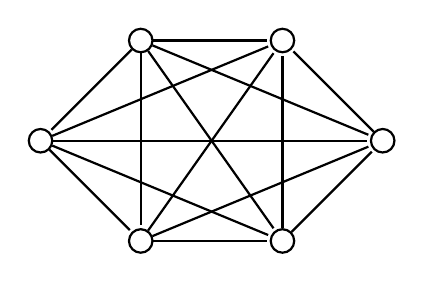
\begin{tikzpicture}[-,>=stealth,shorten >=1pt,auto,node distance=2cm,thick,main node/.style={scale=0.9,circle,draw,font=\sffamily\normalsize}]
            \node[main node] (1) {};
            \node[main node] (2) [below left of=1] {};
            \node[main node] (3) [below right of=2] {};
            \node[main node] (6) [right of=1] {};
            \node[main node] (5) [below right of=6] {};
            \node[main node] (4) [below left of=5] {};

            \path[every node/.style={font=\sffamily\small}]
                (1) edge (2)
                (1) edge (3)
                (1) edge (4)
                (1) edge (5)
                (1) edge (6)

                (2) edge (3)
                (2) edge (4)
                (2) edge (5)
                (2) edge (6)

                (3) edge (4)
                (3) edge (5)
                (3) edge (6)

                (4) edge (5)
                (4) edge (6)

                (5) edge (6)
                ;
        \end{tikzpicture}

        \caption{The complete graph $K_6$ is $5$-connected. In general, $K_{t+1}$ is $t$-connected.}
    \end{figure}

    We observe that the standard notion of connectivity is trivially equivalent to the notion of 1-connectivity since the only subset of vertices that has less than 1 vertex is the empty set. Not-so-surprisingly, $k$-connectivity is strictly related to Menger's theorem. This relation is expressed through the following theorem.

    \begin{framedthm}[label=menger_k_conn]{Menger's theorem (connectivity version)}
        A graph $G$ is $k$-connected if and only if for each distinct $x,y \in V(G)$ there are at least $k$ internally disjoint $(x,y)$ paths.

        \textit{Note}: two paths are internally disjoint if their internal vertices don't intersect.
    \end{framedthm}

    \begin{proof}
        Suppose that $G$ is $k$-connected. For any distinct pair $x,y \in V(G)$ we have two cases:
        \begin{itemize}
            \item If $x \not\sim y$ then, since $G$ is $k$-connected, it must hold that $\delta \geq k$, thus $N(x)$ and $N(y)$ contain at least $k$ vertices. By \Cref{menger}, there are at least $k$ disjoint $N(x), N(y)$ paths. By adding the edges to $x$ and $y$ on each of these paths, we get at least $k$ internally disjoint $(x,y)$ paths. 
            
            \item If $x \sim y$ then $G-\{xy\}$ is $k-1$ connected. Again, by \Cref{menger}, there are at least $k-1$ disjoint $N(x), N(y)$ paths. By adding the edges to $x$ and $y$ on each of these paths, we get at least $k$ internally disjoint $(x,y)$ paths. The final path is given by the edge $xy$.
        \end{itemize}
        
        Vice versa, if a graph $G$ contains $k$ internally disjoint paths between any two
        vertices, then $\abs{G} > k$ and $G$ cannot be separated by fewer than $k$ vertices, thus $G$ is $k$-connected.
    \end{proof}

    In general, when a graph is $k$-connected, lot's of information on the structure of the graph can be inferred, such as the existence of paths, cycles and topological minors. To give an idea behind how these structural information can be derived, we'll list a series of results 

    \begin{framedprop}[label={k_conn_path_cycle}]{}
        Let $G$ be a $k$-connected graph. Then:
        \begin{enumerate}
            \item $\delta(G) \geq k$
            \item Given $A,B \subseteq V(G)$ with $\abs{A}, \abs{B} \geq k$, there are at least $k$ vertex-disjoint $(A,B)$ paths.
            \item Given $x \in V(G)$ and $Y \subseteq V(G)$ with $\abs{Y} \geq k$, there are at least $k$ paths $P_1, \ldots, P_k$ from $x$ to $Y$ that intersect only in $x$.
            \item If $k \geq 2$, given $x_1, \ldots, x_k \in V(G)$ there is a cycle $C$ that passes through $x_1, \ldots, x_k$ in some order.
            \item If $k = 10t$ for some $t \in \N$, given $x_1, \ldots, x_k \in V(G)$ there is a cycle $C$ that passes through $x_1, \ldots, x_k$ in any order.
        \end{enumerate}
    \end{framedprop}

    \begin{proof}
        \quad

        \begin{enumerate}
            \item By way of contradiction, suppose that there is a vertex $x \in V(G)$ such that $\deg(x) < k$. Then, the set $N(x)$ is a set with less than $k$ vertices that disconnects $G$, contradicting the $k$-connectivity of $G$ 
            \item By contrapositive, suppose that there are two subsets $A,B$ with $\abs{A}, \abs{B} \geq k$ and less than $k$ disjoint $(A,B)$ paths. By \Cref{menger}, there exists an $(A,B)$ separation $X,Y$ of order less than $k$. Thus, $X \cap Y$ is an hitting set with less than $k$ vertices. Moreover, we know that $\abs{X} \geq \abs{A} \geq k$ and $\abs{X \cap Y} < k$, thus there is at least one vertex in $X- Y$, concluding that such vertex is disconnected in $G-(X \cap Y)$, hence $G$ is not $k$-connected.
            
            \item Proof similar to the previous point.
            \item Let $X = \{x_1, \ldots, x_k\}$. Let $C$ be a cycle containing as many vertices chosen from $X$ as possible. By way of contradiction, suppose that there is a vertex $x_v \in X$ that isn't covered by $C$. By the previous point, there are at least $k$ paths $P_1, \ldots, P_k$ from $x_v$ to $V(C)$ that intersect only in $x_v$. Since $C$ contains at most $k-1$ vertices chosen from $x_1, \ldots, x_k$, by the pigeonhole principle there must be a subpath $Q$ in $C$ that doesn't intersect $X$, meaning that $X \subseteq C-Q$. Moreover, there are at least two paths $P_i, P_j$ with the second endpoint in $Q$. Hence, $(C-Q) \cup (Q \cap P_1) \cup (Q \cap P_2) \cup P_1 \cup P_2$ form a cycle $C'$ with more vertices taken from $X$ than $C$, raising a contradiction.
            \item Omitted.
        \end{enumerate}
    \end{proof}

    In some cases, $k$-connectivity can also be used to establish the existence of more complex structures. This is the case of \textbf{topological minors}. Given an edge $xy$, an \textbf{edge subdivision} of $xy$ is obtained by decomposing the edge into two edges $xz$ and $xy$, where $z$ is a new vertex. A \textbf{subdivision} of a graph $G$ is a graph obtained by subdividing at least one edge of $G$.

    \begin{figure}[H]
        \centering

        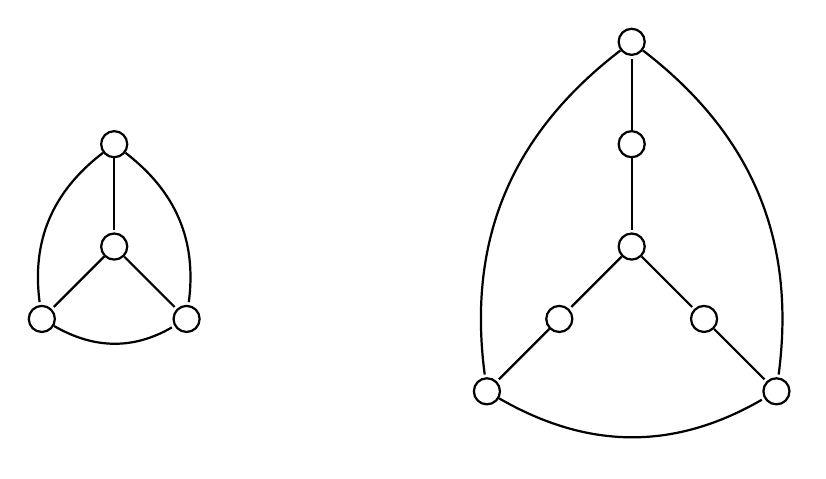
\begin{tikzpicture}[-,>=stealth,shorten >=1pt,auto,node distance=1.3cm,thick,main node/.style={scale=0.9,circle,draw,font=\sffamily\normalsize}]

            \node[circle, draw] (1) []{};
            \node[circle, draw] (2) [below of = 1]{};
            \node[circle, draw] (3) [below left of = 2]{};
            \node[circle, draw] (4) [below right of = 2]{};

                \draw[-] (1) to (2);
                \draw[-] (1) [bend right] to (3);
                \draw[-] (1) [bend left] to (4);
                \draw[-] (2) to (3);
                \draw[-] (2) to (4);
                \draw[-] (3) [bend right] to (4);
            ;

            \node[circle, draw] (1x) [right of = 1, xshift = 150]{};
            \node[circle, draw] (2x) [below of = 1x]{};
            \node[circle, draw] (3x) [below left of = 2x]{};
            \node[circle, draw] (4x) [below right of = 2x]{};
            \node[circle, draw] (5x) [above of = 1x]{};
            \node[circle, draw] (6x) [below left of = 3x]{};
            \node[circle, draw] (7x) [below right of = 4x]{};

                \draw[-] (1x) to (2x);
                \draw[-] (5x) [bend right] to (6x);
                \draw[-] (5x) [bend left] to (7x);
                \draw[-] (2x) to (3x);
                \draw[-] (2x) to (4x);
                \draw[-] (1x) to (5x);
                \draw[-] (3x) to (6x);
                \draw[-] (4x) to (7x);
                \draw[-] (6x) [bend right] to (7x);
            ;
        \end{tikzpicture}

        \caption{The graph $K_4$ (left) and one of its subdivisions of $K_4$ (right).}
    \end{figure}

    \begin{frameddefn}{Topological minor}
        Let $G$ be a graph. A graph $H$ is a \textbf{topological minor} of $G$ if $G$ has a subgraph that is a subdivision of $H$.
    \end{frameddefn}
    
    \begin{figure}[H]
        \centering
        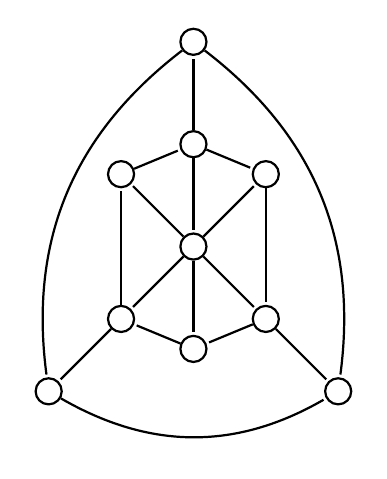
\begin{tikzpicture}[-,>=stealth,shorten >=1pt,auto,node distance=1.3cm, thick,main node/.style={scale=0.9,circle,draw,font=\sffamily\normalsize}]

            \node[circle, draw] (1) []{};
            \node[circle, draw] (2) [below of = 1]{};
            \node[circle, draw] (3) [below left of = 2]{};
            \node[circle, draw] (4) [below right of = 2]{};
            \node[circle, draw] (5) [above of = 1]{};
            \node[circle, draw] (6) [below left of = 3]{};
            \node[circle, draw] (7) [below right of = 4]{};
            \node[circle, draw] (8) [above left of = 2]{};
            \node[circle, draw] (9) [above right of = 2]{};
            \node[circle, draw] (10) [below of = 2]{};

            \draw[-] (1) to (2);
            \draw[-] (5) [bend right] to (6);
            \draw[-] (5) [bend left] to (7);
            \draw[-] (2) to (3);
            \draw[-] (2) to (4);
            \draw[-] (1) to (5);
            \draw[-] (3) to (6);
            \draw[-] (4) to (7);
            \draw[-] (6) [bend right] to (7);
            \draw[-] (2) to (8);
            \draw[-] (2) to (9);
            \draw[-] (2) to (10);

            \draw[-] (8) to (1);
            \draw[-] (1) to (9);
            \draw[-] (9) to (4);
            \draw[-] (4) to (10);
            \draw[-] (10) to (3);
            \draw[-] (3) to (8);

            ;
        \end{tikzpicture}
        \caption{A graph containing $K_4$ as a topological minor.}
    \end{figure}

    \begin{framedprop}[label={k4_topmin}]{}
        If $G$ is a $3$-connected graph then it contains $K_4$ as a topological minor.
    \end{framedprop}

    \begin{proof}
        Since $G$ is $3$-connected, we know that it has at least a vertex and that $\delta(G) \geq 3$. Fix $x \in V(G)$. Since $G-x$ has $\delta(G-x) \geq 2$, by \Cref{delta_cycle} we know that it contains a cycle $C$ of length at least 3. By \Cref{k_conn_path_cycle}, we know that there are three paths $P_1, P_2, P_3$ from $x$ to $V(C)$ that intersect only in $x$. Then, $P_1 \cup P_2 \cup P_3 \cup C$ form a subdivision of $K_4$ in $G$.
    \end{proof}

    \newpage

    \section{Disjoint cycles and feedback vertex sets}

    Similarly to Euler's theorem, as a corollary to Menger's theorem we get that the problem that asks to determine the existence of $k$ disjoint paths in a graph lies in the intersection $\mathsf{NP} \cap \mathsf{coNP}$ since the theorem gives us a polynomially verifiable condition both for existence and non-existence of the tour. In fact, the problem actually lies in the class $\mathsf{P}$ by reduction to the \textit{max-flow problem}.

    A very similar problem asks to deterine the existence of $k$ disjoint cycles in a graph. This problem, however, is $\mathsf{NP}$-complete. Nonetheless, many results are able to assert the existence of a number of disjoint cycles when some conditions are met. These results will be discussed in the following section.

    \begin{framedprop}[label=3reg_cycle]{}
        Let $G$ be a multigraph. If $G$ is 3-regular then it contains a cycle of length at most $2\ceil{\log n}$
    \end{framedprop}

    \begin{proof}
        If $G$ contains a loop or parallel edges (or multi-edges), the proposition trivially holds. Thus, we may assume to be working with simple graphs. Fix a vertex $v \in V(G)$. Consider a BFS on $G$ that starts from $v$ and goes on until no cycles of length at most $2\ceil{\log n}$ are encountered. Let $T$ be the tree produced by such BFS. Since $G$ is 3-regular, $v$ will have three children in $T$ and each of those children will be the root of a binary tree inside in $T$. In other words, all the other nodes in the tree (except the leaves) will have two children.
        
        If the BFS stops before visiting the whole graph, the proposition holds. Hence, we may assume that the BFS doesn't stop, implying that $V(T) = V(G)$. By 3-regularity of $G$, we know that $\delta = 3$, hence by \Cref{delta_cycle} we get that there must be a cycle in $G$. By definition of BFS, this cycle must connect two leaves $x,y \in V(T)$ through an edge, otherwise the algorithm wouldn't have taken the shortest path on one of the two branches. Therefore, this cycle must be formed by the edge $xy$ and the paths from $x$ to $z$ and from $y$ to $z$, where $z$ is the \textit{lowest common ancestor} of $x$ and $y$.

        Since $T$ contains $n$ nodes and by definition of BFS it is a balanced tree, the height of $T$ is at most $\ceil{\log n} -1$. Hence, the two paths can have length at most $\ceil{\log n} -1$, concluding that the cycle has length at most $2\ceil{\log n} -1 \leq 2\ceil{\log n}$
    \end{proof}

    The above proposition works only for 3-regular graphs, but out final result will involve any type of graph. We give a definition of graphs that are not too far away from being 3-regular.

    \begin{frameddefn}{3-graph with discrepancy $d$}
        A 3-graph $G$ of discrepancy $d$ is a multigraph such that $\Delta \leq 3$ and:
        \[\sum_{v \in V(G)} 3-\deg(v) \leq d\]
        By definition, a 3-graph of discrepancty 0 is a 3-regular graph. 
    \end{frameddefn}

    We define the inverse operation of \textit{edge subdivision} as \textbf{vertex suppression}. Given a vertex $v$ of degree 2, suppressing $v$ means to remove $v$ and join its two neighbors with an edge. For verteices of degree 1, instead, suppressing $v$ means removing $v$.

    \begin{framedprop}{}
        Let $G$ be a 3-graph with discrepancy $d$. Then, there is a sequence of at most $d$ operations chosen from:
        \begin{itemize}
            \item suppression of a vertex of degree 2
            \item suppression of a vertex of degree 1
            \item deletion of a vertex of degree 0
        \end{itemize}

        that results in a 3-regular graph.
    \end{framedprop}

    \begin{proof}
        We proceed by induction on $d$. When $d = 0$, the initial graph already has discrepancy 0 so no operations have to be applied. Assume the inductive hypothesis for $d-1$ and consider the case $d$. Since $G$ has discrepancy at least 1, at least one vertex $v$ has degree at most 2. We have three cases:
        \begin{itemize}
            \item If $\deg(v) = 0$ then by removing $v$ we get a graph with discrepancy $d-3$ since the degree difference decreases by $3+0$ due to removal of $v$:
            \[\sum_{v \in V(G-x)} 3-\deg(v) = -3 + \sum_{v \in V(G)} 3-\deg(v) \leq d-3 \leq d-1\]
            \item If $\deg(v) = 1$ then by suppressing $v$ we get a graph $H$ with discrepancy $d-1$ since the degree difference decreases by $3-1$ due to the removal of $v$ and the degree of its neighbor gets decreased by 1:
            \[\sum_{v \in V(H)} 3- \deg(v) = -1 + \sum_{v \in V(G)} 3-\deg(v) \leq d-1\]
            \item If $\deg(v) = 2$ then by suppressing $v$ we get a graph $H$ with discrepancy $d-1$ since the degree difference decreases by $3-2$ due to the removal of $v$ and the degree of its neighbors is unchanged:
            \[\sum_{v \in V(H)} 3- \deg(v) = -1 + \sum_{v \in V(G)} 3-\deg(v) \leq d-1\]
        \end{itemize} 

        In all three cases, by applying the inductive hypothesis we conclude the proof.
    \end{proof}

    \begin{framedlem}{}
        There is a constant $c > 0$ such that for any $k \in \N$ for any 3-regular multigraph $G$ with $\abs{V(H)} \geq ck\log(k+1)$ then there are at least $k$ vertex-disjoint cycles in $G$.
    \end{framedlem}

    \begin{proof}
        We proceed by induction on $k$. When $k = 1$, since $G$ is 3-regular we have that $\delta(G) = 3$. By \cref{delta_cycle}, we conclude that $G$ contains a cycle. Assume the inductive hypothesis for $k-1$ and consider the case $k$. Again, since $G$ is 3-regular it must contain at least a cycle. Let $C$ be the shortest cycle in $G$. Since $\abs{V(G)} \geq ck \log (k+1)$, by \Cref{3reg_cycle} we have that:
        \[\abs{V(C)} \leq 2 \ceil{\log (ck\log(k+1))} \leq 2 \log(ck\log(k+1)) + 2\]

        Consider now the graph $G-C$. Since we removed edges, this graph is a 3-graph with discrepancy $d$ for some constant $d$. By the previous proposition, we know that $G-C$ can be suppressed into a 3-regular graph $G'$. Moreover, we have that:
        \[\abs{V(G')} \geq \abs{V(G)} - 2 \abs{V(C)} \geq ck\log(k+1) - 4 \log(ck\log(k+1)) + 4 \geq c(k-1)\log k\]

        Thus, by inductive hypothesis we have that $G'$ contains at least $k-1$ disjoint cycles, which implies that also $G-C$ does. Since $C$ is disjoint from all those cycles, we get that $G$ contains at leasts $k$ disjoint cycles.
    \end{proof}

    \textcite{erdos_posa} proved that the number of disjoint cycles in a graph is strictly related the size of \textbf{feedback vertex sets}, that being subset of vertices that intersect every cycle of the graph $G$.

    \begin{frameddefn}{Feedback vertex set}
        Let $G$ be a graph. A subset $X \subseteq V(G)$ is called \textbf{feedback vertex set (FVS)} if every cycle of $G$ contains a vertex of $X$. Equivalently, $G-X$ is acyclic.
    \end{frameddefn}

    \begin{figure}[H]
        \centering
        \begin{tikzpicture}[-,>=stealth,shorten >=1pt,auto,node distance=1.5cm,thick,main node/.style={scale=0.9,circle,draw,font=\sffamily\normalsize}]

            \node[circle, draw] (1) []{};
            \node[circle, draw, fill=Carmine] (2) [right of = 1]{};
            \node[circle, draw] (3) [below right of = 2]{};
            \node[circle, draw] (4) [below left of = 3]{};
            \node[circle, draw] (5) [left of = 4]{};
            \node[circle, draw, fill=Carmine] (6) [above left of = 5]{};

            \node[circle, draw, fill=Carmine] (7) [right of = 3]{};
            \node[circle, draw] (8) [above right of = 7]{};
            \node[circle, draw] (9) [below right of = 7]{};

            \draw[-] (1) to (2);
            \draw[-] (2) to (3);
            \draw[-] (3) to (4);
            \draw[-] (4) to (5);
            \draw[-] (5) to (6);
            \draw[-] (6) to (1);

            \draw[-] (3) to (7);
            \draw[-] (7) to (8);
            \draw[-] (8) to (9);
            \draw[-] (9) to (7);

            \draw[-] (1) to (4);
            \draw[-] (2) to (5);

            ;
        \end{tikzpicture}
        \caption{The ref vertices form a feedback vertex set.}
    \end{figure}

    \newpage

    \begin{framedthm}{Erdős-Pósa theorem}
        There is a constant $c > 0$ such that any $k \in \N$ and any graph $G$ it holds that $G$ either has at least $k$ vertex-disjoint cycles or there is a FVS $X$ such that $\abs{X} \leq ck\log k$.
    \end{framedthm}

    \begin{proof}
        If G contains at least $k$ disjoint cycles, the theorem is trivially true. Moreover If $G$ is acyclic, the empty set is an FVS that satisfies the theorem. Thus, we may assume that $G$ contains at least one cycle but less than $k$ disjoint cycles.
        
        Let $H$ be a maximal subgraph of $G$ such that $2 \leq \delta(H) \leq \Delta(H) \leq 3$. We observe that such subgraph $H$ always exists since $G$ contains at least one cycle. Let $C_{i_1}, \ldots, C_{i_t}$ be the cycle components of $H$, i.e. the components of $H$ that are cycles. For each $j \in [t]$, let $x_{j}$ be a vertex of $C_{i_{j}}$. Let $W = \{x_{j} \mid j \in t\}$. Since $G$ has less than $k$ disjoint cycles, $H$ contains less than $k$ cycle components, implying that $\abs{W} \leq k+1$.
        
        Let $H'$ be the subgraph obtained by removing all the cycle components from $H$. Then, $H'$ is a subdivision of a 3-regular graph. Furthermore, since $G$ contains less than $k$ disjoint cycles, by the previous lemma $H$ must contain less than $c'k\log(k+1)$ vertices, for some constant $c' > 0$. Let $\mathcal{U} = \{v \in V(H') \mid \deg_{H'}(v) = 3\}$. We have that $\abs{\mathcal{U}} < c'k\log(k+1)$.

        \textbf{Claim 1}: every cycle of $G$ intersects $H$.

        \begin{proof}[Proof of Claim 1]
            By way of contradiction, suppose that there is a cycle $C$ of $G$ that doesn't intersect $H$. Then, since every vertex of $C$ has degree 2, $H \cup C$ contradicts the maximality of $H$. 
        \end{proof}

        \textbf{Claim 2}: there are no paths in $G-(\mathcal{U} - W)$ of length at least 1 such that all of the following hold:
        \begin{itemize}
            \item both endpoints are in $H-(\mathcal{U} - W)$
            \item no internal vertex is in $H$
            \item no edge is in $H$
        \end{itemize}

        \begin{proof}[Proof of Claim 2]
            By way of contradiction, suppose that there is a path $P$ with all of these properties. Then, since every vertex of $P$ has degree 2, no edge and no internal vetex of $P$ lies in $H$, the graph $H \cup C$ contradicts the maximality of $H$. 
        \end{proof}

        \textbf{Claim 3}: every cycle of $G-(\mathcal{U} \cup W)$ intersects $H$ in exactly one vertex.

        \begin{proof}[Proof of Claim 3]
            Through Claim 1, we know that every cycle of $G$ must intersect $H$ in at least 1 vertex, hence this also holds for cycles of $G-(\mathcal{U} \cup W)$. By way of contradiction, suppose that there is a cycle $C$ of $G-(\mathcal{U} \cup W)$ that intersects $H$ in at least two vertices. The cycle $C$ can be partitioned into edge disjoint paths $P_1, \ldots, P_v$ such that the ends of each $P_i$ are in $C \cap H$ and no internal vertex of $P_i$ is in $H$. Since $C$ has at least two vertices, we know that $v \geq 2$.

            We observe that it may be possible for some $P_i$ to be a single edge in $H$, but at least one of $P_1, \ldots, P_v$ must be. However, since $C \subseteq G-(\mathcal{U}-W)$ and since $H-(\mathcal{U}-W)$ is acyclic, this single edge path violates Claim 2, raising a contradiction.
        \end{proof}

        Let $Z \subseteq V(H-(\mathcal{U}-W))$ be the set of vertices $z$ for which there is a cycle $C$ of $G-(\mathcal{U} \cup W)$ such that $C \cap H = \{z\}$. We observe that given $z,z' \in Z$ such that $z \neq z'$, the two cycles $C,C'$ in $G-(\mathcal{U} \cup W)$ such that $C \cap H = \{z\}$ and $C' \cap H = \{z'\}$ must be disjoint, otherwise there would be a path from $v_1$ to $v_2$ that contradicts Claim 2. Furthermore, since there are at most $k-1$ cycles, we conclude that $\abs{Z} \leq k-1$.

        By construction of $\mathcal{U},W,Z$ and by all the claims that we proved, we get that $X = \mathcal{U} \cup W \cup Z$ is a FVS of $G$. Moreover, we have that:
        \[\begin{split}
            \abs{X} &\leq \abs{\mathcal{U}} + \abs{W} + \abs{Z} \\
            &< c'k\log (k+1) + k-1 + k-1 \\
            &\leq ck \log k
        \end{split}\]

        for some $c > 0$, concluding the proof.
    \end{proof}
    

    \section{Directed graphs and path covers}

    Up until now, we have discussed only \textit{undirected graphs}. In this section, we'll shift our focus to \textit{directed graphs} (or \textit{digraphs}), that being graphs whose edges are oriented, implying that the edge $(x,y)$ is not equal to the edge $(y,x)$. We gave a formal definition of directed graphs in \Cref{graphs}. In particular, we'll focus on determining the existence of \textbf{path covers}, i.e. sets of disjoint directed paths that cover every vertex of the graph. 

    \begin{frameddefn}{Path cover}
        Let $G$ be a digraph. A \textbf{path cover} for $G$ is a set $\mathcal{P}$ of disjoint paths such that $V(G) = \cup_{P \in \mathcal{P}} V(P)$.
    \end{frameddefn}

    \begin{figure}[H]
        \centering
        \begin{tikzpicture}[->,>=stealth,shorten >=1pt,auto,node distance=2cm,thick,main node/.style={scale=0.9,circle,draw,font=\sffamily\normalsize}]
            \node[main node] (1) {};
            \node[main node] (2) [below left of=1] {};
            \node[main node] (3) [below right of=2] {};
            \node[main node] (6) [right of=1] {};
            \node[main node] (5) [below right of=6] {};
            \node[main node] (4) [below left of=5] {};

            \path[every node/.style={font=\sffamily\small}]
                (1) edge [bend left, color=Carmine, line width=2](2)
                (2) edge [bend left] (1)
                (2) edge [color=Carmine, line width=2](3)
                (2) edge (4)
                (3) edge [color=Carmine, line width=2](4)
                (4) edge [bend left](3)
                (1) edge (4)
                (1) edge (5)
                (6) edge (3)
                (6) edge [color=Carmine, line width=2](5)
                ;
        \end{tikzpicture}

        \caption{The red paths form a path cover.}
    \end{figure}

    We observe that any digraph contains a trivial path cover, that being the cover formed by the set of every single-vertex path. We're interested in finding the minimum cardinality path cover. \textcite{gallai} proved that path covers are strictly related to \textit{independent sets}.

    \begin{framedthm}{Gallai-Milgram theorem}
        For every digraph $G$, there is a path cover $\mathcal{P}$ of $G$ and an independent set $X$ such that $\abs{X \cap P} = 1$ for all $P \in \mathcal{P}$.
    \end{framedthm}

    We prove a slightly stronger result that directly implies the above theorem. Given a path cover $\mathcal{P}$, we define $\mathrm{ter}(\mathcal{P})$ as the set of terminal nodes of the paths in $\mathcal{P}$.
    \[\mathrm{ter}(\mathcal{P}) = \{v \in V(G) \mid \exists P \in \mathcal{P} \text{ s.t. } v \in V(P), \mathrm{our-deg}_P (v) = 0\}\]

    We say that a path cover $\mathcal{P}$ is \textit{minimal by inclusion} if there is no other path cover $\mathcal{P}'$ whose terminal nodes are a strict subset of the terminal nodes of the former, i.e. $\mathrm{ter}(P') \subset \mathrm{ter}(P)$.

    \begin{framedprop}{}
        Let $G$ be a digraph and let $\mathcal{P}$ be a path cover of $G$ that is minimal by inclusion. Then, there is an independent set $X$ such that $\abs{X \cap P} = 1$ for all $P \in \mathcal{P}$.
    \end{framedprop}

    \begin{proof}
        We proceed by induction on $n$. If $n = 1$, we trivially have that the single node in $G$ forms both the path cover and the independent set. Assume the inductive hypothesis and consider $n>1$. We may assume that $\mathrm{ter}(\mathcal{P})$ is not an independent set, since otherwise the proof trivially follows.

        Let $\mathcal{P} = \{P_1, P_2, \ldots, P_k\}$. For each $i \in [k]$, let $x_i$ be the terminal of $P_i$. Since $\mathrm{ter}(\mathcal{P})$ is not an independent set, there is at least one edge between the terminals of two paths in the cover. Without loss of generality, assume that such edge is $(x_2,x_1) \in E(G)$. Consider the set $\mathcal{P}' = \{P_1 - x_1, P_2, \ldots, P_k\}$. This set is clearly a path cover for $G-x$.
        
        \textbf{Claim:} $\mathcal{P}'$ is minimal by inclusion for $G-x$.

        \begin{proof}[Proof of the claim]
            By way of contradiction, suppose that $\mathcal{P}'$ is not minimal by inclusion for $G-x$. Then, there must be another path cover $\mathcal{P}^*$ for $G-x$ such that $\mathrm{ter}(\mathcal{P}^*) \subset \mathrm{ter}(\mathcal{P}')$.

            We observe that the path $P_1$ must contain at least 2 nodes, otherwise $\mathcal{P}'' = (\mathcal{P}-\{P_1\}) \cup \{P_2 \cup (x_2,x_1)\}$ is a path cover for $G$ such that $\mathrm{ter}(P'') \subset \mathrm{ter}(\mathcal{P})$, contradicting the minimality by inclusion of $\mathcal{P}$. Thus, the node $x_1'$ that is adjacent to $x_1$ in $P_1$ must be the new terminal of $P_1-x_1$, concluding that $\mathrm{ter}(\mathcal{P}') = \{x_1', x_2, \ldots, x_k\}$.

            Since $\mathrm{ter}(\mathcal{P}^*) \subset \{x_1', x_2, \ldots, x_k\}$, we hvae three cases:
            \begin{enumerate}
                \item $x_1' \in \mathrm{ter}(\mathcal{P}^*)$. Then, there is a $x_j \in \mathrm{ter}(\mathcal{P}')- \mathrm{ter}(\mathcal{P}^*)$ such that $x_j \neq x_1'$. Let $Q_1'$ be the path in $\mathcal{P}^*$ ending in $x_1'$. Then, the set 
                \[\mathcal{P}^{\#} = (\mathcal{P} - Q_1') \cup (Q_1' \cup (x_1',x_1))\]
                is a path cover for $G$ with $\mathrm{ter}(P^{\#}) \subset \mathrm{ter}(\mathcal{P})$, contradicting the minimality by inclusion for $G$ of $\mathcal{P}$.

                \item $x_1' \notin \mathrm{ter}(\mathcal{P}^*)$ and $x_2 \in \mathrm{ter}(\mathcal{P}^*)$. Let $Q_2$ be the path in $\mathcal{P}^*$ ending in $x_2$. Then, the set
                \[\mathcal{P}^{\#} = (\mathcal{P} - Q_2) \cup (Q_2 \cup (x_2,x_1))\]
                is a path cover for $G$ with $\mathrm{ter}(P^{\#}) \subset \mathrm{ter}(\mathcal{P})$, contradicting the minimality by inclusion for $G$ of $\mathcal{P}$.

                \item $x_1' \notin \mathrm{ter}(\mathcal{P}^*)$ and $x_2 \notin \mathrm{ter}(\mathcal{P}^*)$. Then, the set 
                \[\mathcal{P}^{\#} = \mathcal{P} \cup \{x_1\}\]
                is a path cover for $G$ with $\mathrm{ter}(P^{\#}) \subset \mathrm{ter}(\mathcal{P})$, contradicting the minimality by inclusion for $G$ of $\mathcal{P}$.
            \end{enumerate}
        \end{proof}

        Since $\mathrm{ter}(\mathcal{P}')$ is minimal by inclusion for $G-x$, by inductive hypothesis we get that there is an independent set $X$ such that $\abs{X \cap P_i} = 1$ for all $i \in [k]$, concluding that $X$ also satisfies the theorem for $G$.
    \end{proof}

    \begin{framedcor}{}
        Let $G$ be a digraph. Then, the minimum cardinality of a path cover for $G$ is at most the maximum cardinality of an independent set for $G$.
    \end{framedcor}

    \begin{proof}
        By way of contradiction, suppose that the minimum cardinality of a path cover $\mathcal{P}$ for $G$ is greater than the maximum cardinality of an independent set $X$ for $G$. Then, by the previous theorem, there must be an independent set $X'$ such that $\abs{X' \cap P} = 1$ for all $P \in \mathcal{P}$. Since every path in $\mathcal{P}$ is disjoint, $X'$ must have at least $\abs{\mathcal{P}}$ vertices, implying that $\abs{X} < \abs{\mathcal{P}} \leq \abs{X'}$ and thus contradicting the choice of $X$.
    \end{proof}

    The above corollary gives us a lower bound for the maximum independent set problem, which is known to be $\mathsf{NP}$-hard. However, it's easy to see that a graph contains an Hamiltoniam path if and only if there is a path cover made of one single path, concluding that the former problem can be reduced to the latter, making the minimum path cover problem also $\mathsf{NP}$-hard.
    
    Nonetheless, the Gallai-Milgram theorem still has some applications in other branches of mathematics. For instance, it can be used to get a short proof of a result originally proved -- using different techniques -- by \textcite{dilworth} involving \textit{partially ordered sets} (or \textit{posets}). Given a poset $(S, \prec)$ , we define a \textbf{chain} as a sequence of pairwise comparable elements, such as $a_1 \prec a_2 \prec \ldots \prec a_k$. We define an \textbf{anti-chair} as a set of incomparable elements, i.e. such that $\forall x,y$ it holds that $x \not\prec y$ and $y \not\prec y$.

    \begin{figure}[H]
        \centering
        \begin{tikzpicture}[<-,>=stealth,shorten >=1pt,auto,node distance=2cm,thick,main node/.style={scale=0.9,circle,draw,font=\sffamily\normalsize}]
            \node[] (1) {$\{1,2,3\}$};
            \node[] (2)[below of = 1] {$\{2,3\}$};
            \node[] (3)[left of = 2] {$\{1,2\}$};
            \node[] (4)[right of = 2] {$\{1,3\}$};

            \node[rectangle, draw = BlueLagoon, line width = 2] (5)[below of = 2] {$\{1\}$};
            \node[rectangle, draw = BlueLagoon, line width = 2] (6)[below of = 3] {$\{2\}$};
            \node[rectangle, draw = BlueLagoon, line width = 2] (7)[below of = 4] {$\{3\}$};
            \node[] (8)[below of = 5] {$\varnothing$};


            \path[every node/.style={font=\sffamily\small}]
                (1) edge (2)
                (1) edge[color = Carmine, line width = 2] (3)
                (1) edge (4)

                (2) edge (6)
                (2) edge (7)
                (3) edge (5)
                (3) edge[color = Carmine, line width = 2] (6)
                (4) edge (5)
                (4) edge (7)

                (5) edge (8)
                (6) edge[color = Carmine, line width = 2] (8)
                (7) edge (8)
                ;
        \end{tikzpicture}

        \caption{The poset $(\{1,2,3\}, \subseteq)$ (transitive and reflexive edges are omitted). The red path forms a chain, while the blue rectangles form an anti-chain.}
    \end{figure}

    \begin{framedthm}{Dilworth's theorem}
        In every poset $(S, \prec)$, the minimum number of chains covering $S$ is equal to the maximum cardinality of an antichain.
    \end{framedthm}

    \begin{proof}
        Let $(S,\prec)$ be a poset. Let $c(S)$ denote the minimum number of chains that cover $S$ and let $a(S)$ be the maximum cardinality of an anti-chain in $S$. We construct the graph $G_S$ such that $V(G_S) = S$ and $E(G) = \{(x,y) \mid x \prec y\}$. By construction, each chain in $S$ corresponds to a path in $G_S$. Similarly, each anti-chain in $S$ corresponds to a set of disconnected nodes, i.e. nodes for which there is no path that connects them. By definition, each set of disconnected nodes is also an inpendendent set. Thus, by the Gallai-Milgram theorem we get that:
        \[c(S) = \abs{\mathcal{P}^*} \leq \abs{X^*} \leq a(S)\]

        where $\mathcal{P}^*$ is a minimum path cover and $X^*$ is a maximum independent set. Moreover, for each path cover there must be at least a path for each node in a set of disconnected nodes, concluding that $c(S) \geq a(S)$ also holds.
    \end{proof}

    \newpage

    \section{Solved exercises}

    \begin{framedprob}{}
        Prove that any $t$-connected subgraph $G$ with $n \geq t+2$ contains $K_{2,t}$ as a topological minor.
    \end{framedprob}

    \begin{proof}[Solution]
        We may assume that $G \neq K_n$ since otherwise $G$ contains $K_{2,t}$ as a subgraph, hence as a topological minor. Let $x,y \in V(G)$ be two vertices such that $x \not\sim y$. Since $G$ is $t$-connected, we know that $\delta \geq t$, hence $\abs{N(x)}, \abs{N(y)} \geq t$. By Menger's theorem, there are at least $t$ disjoint paths from $N(x)$ to $N(y)$ since otherwise we would have a separation that contradicts the $t$-connectivity of $G$.
        
        Let $P_1, \ldots, P_t$ be $t$ of those paths. For each $i \in [t]$, let $x_i$ be the endpoint of $P_i$ lying in $N(x)$ and let $y_i$ be the one lying in $N(y)$. Then, the graph given by
        \[\bigcup_{i = 1}^t xx_i \cup P_i \cup y_iy\]
        is a subdivision of $K_{2,t}$ since each internal vertex of $P_i \cup \{y_i, y\}$ can be suppressed, obtaining an edge from $y$ to $x_i$.
    \end{proof}

    \begin{framedprob}{}
        Let $G$ be a 3-connected subgraph and let $xy$ be an edge of $G$. Prove that $G/xy$ is 3-connected if and only if $G-\{x,y\}$ is 2-connected.
    \end{framedprob}

    \begin{proof}[Solution]
        We use the characterization of $k$-connectivity given by \Cref{menger_k_conn}. Let $z$ be the vertex given by the contraction of $xy$. We split the proof in two claims.

        \textbf{Claim 1}: if $G/xy$ is 3-connected then $G-\{x,y\}$ is 2-connected.

        \begin{proof}[Proof of Claim 1]
            Suppose that $G/xy$ is 3-connected. Fix two vertices $u,v \in V(G-\{x,y\})$. Since $G/xy$ is 3-connected and $z,w \in V(G-\{x,y\}) \subseteq V(G/xy)$, there are at least 3 internally disjoint paths $P_1, P_2, P_3$ from $u$ to $v$. If $z \notin V(P_1 \cup P_2 \cup P_3)$ then the three paths are also paths of $G-\{x,y\}$. Hence, we may assume that $z \in V(P_1 \cup P_2 \cup P_3)$. 
            
            Then, exactly one of the paths passes through $z$ since they are internally disjoint. Without loss of generality, let $P_1$ be such path. Let $P_1^{xy}$ denote the path induced by $P_1$ in $G$ after de-contracting $xy$. Since $z \in V(P_1)$, at least one between $x$ and $y$ lies inside $P_1^{xy}$. Moreover, the second vertex cannot lie inside $P_2^{xy},P_3^{xy}$, since otherwise $P_1, P_2,P_3$ wouldn't be internally disjoint. This concludes that $P_1^{xy}, P_2^{xy}, P_3^{xy}$ are three internally disjoint paths in $G-\{x,y\}$ that connect $u$ and $v$, concluding that $G-\{x,y\}$ is 2-connected.
        \end{proof}
        
        \textbf{Claim 2:} if $G-\{x,y\}$ is 2-connected then $G/xy$ is 3-connected

        \begin{proof}[Proof of Claim 2]
            Suppose that $G-\{x,y\}$ is 2-connected. Fix two vertices $s,t \in V(G)$. Since $G$ is 3-connected, there are at least 3 internally disjoint paths $Q_1, Q_2, Q_3$ from $s$ to $t$. Since $G-\{x,y\}$ is 2-connected, at least one of such paths must be impossible to take in $G-\{x,y\}$, which can happen only if it passes through $x$ or $y$. Moreover, there can be at least another such path since otherwise $Q_1, Q_2, Q_3$ wouldn't be internally disjoint.
        
            Suppose that there is only one path crossing $x$ or $y$. Without loss of generality, assume that $Q_1$ is such path, implying that $Q_2,Q_3$ are paths of $G/xy$ from $s$ to $t$. If $x,y \in V(Q_1)$, the path $Q_1 / xy$ forms the third path in $G/xy$ from $s$ to $t$. If $x \in V(Q_1)$ and $y \notin V(Q_1)$, the path $(Q_1 - \{x\}) \cup \{z\}$ forms the third path in $G/xy$ from $s$ to $t$. The case $x \in V(Q_1)$ and $y \notin V(Q_1)$ is similar to the latter one.

            Suppose now that there are two paths crossing $x$ or $y$. Without loss of generality, assume that $Q_1,Q_2$ are such paths, implying that $Q_3$ is a path of $G/xy$ from $s$ to $t$. We also assume that $Q_1$ is the path crossing $x$ and that $Q_2$ is the one crossing $y$. Then, there must be another path $Q'$ in $G$ that goes from $s$ to $t$, since otherwise $G-\{x,y\}$ wouldn't be 2-connected due to $Q_1$ and $Q_2$ being impossible to take. Moreover, by contracting $xy$ the two paths get joined together, but we're still able to traverse them. Thus, $Q'' = (Q_1 -\{x\}) \cup \{z\}$ is another path from $s$ to $t$, for a total of 3 internally disjoint paths, that being $Q_3, Q'$ and $Q''$.
        \end{proof}
    \end{proof}

    \begin{framedprob}{}
        Prove that every 3-connected graph has a cycle of even lenght. Show that there is a 3-connected graph that has no cycle of odd lenght.
    \end{framedprob}

    \begin{proof}
        Let $G$ be a 3-connected graph and consider two nodes $x,y \in V(G)$. By \Cref{k_conn_path_cycle}, there are at least three internally disjoint paths $P_1, P_2, P_3$ from $x$ to $y$. We may assume that $\abs{P_1 \cup P_2} = 2k+1$ and $\abs{P_2 \cup P_3} = 2h+1$, i.e. that they are odd cycles, otherwise the result trivially follows. However, this implies that:
        \[\abs{P_1 \cup P_3} = \abs{P_1 \cup P_2} + \abs{P_2 \cup P_3} - 2\abs{P_2} = 2k+1 + 2h+1 - 2 \abs{P_2} = 2(k+h+1+ \abs{P_2})\]
        concluding that it is an even cycle.
    \end{proof}

    \begin{figure}[H]
        \centering
        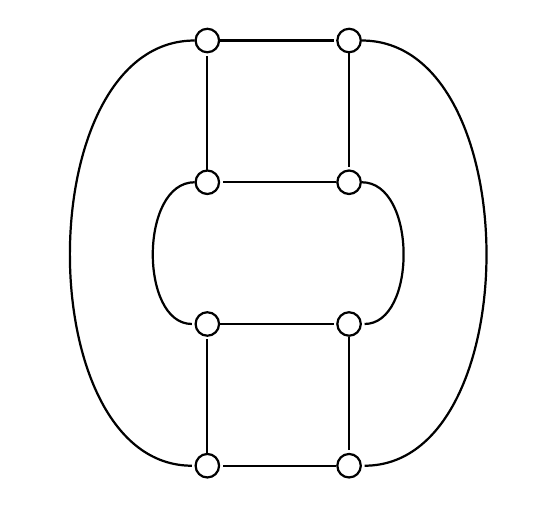
\begin{tikzpicture}[-,>=stealth,shorten >=1pt,auto,node distance=2cm,thick,main node/.style={scale=0.9,circle,draw,font=\sffamily\normalsize}]
            \node[main node] (1) []{};
            \node[main node] (2) [right of = 1]{};
            \node[main node] (3) [below of = 2]{};
            \node[main node] (4) [left of = 3]{};

            \node[main node] (5) [below of = 4]{};
            \node[main node] (6) [right of = 5]{};
            \node[main node] (7) [below of = 6]{};
            \node[main node] (8) [left of = 7]{};
            
            \path[every node/.style={font=\sffamily\small}]
                (1) edge (2)
                (2) edge (3)
                (3) edge (4)
                (4) edge (1)
                
                (5) edge (6)
                (6) edge (7)
                (7) edge (8)
                (8) edge (5)

                (1) edge[out = 180, in = 180] (8)
                (4) edge[out = 180, in = 180] (5)
                (2) edge[out = 0, in = 0] (7)
                (3) edge[out = 0, in = 0] (6)
            ;
        \end{tikzpicture}

        \caption{A 3-connected graph without odd length cycles.}
    \end{figure}

    \begin{framedprob}{}
        Given a graph $G$, let $\alpha(G)$ denote the largest size of a set of independent vertices in $G$. Prove that the vertices of $G$ can be covered by at most $\alpha(G)$ disjoint subgraphs each being either a cycle, an edge or a single vertex.
    \end{framedprob}

    \begin{proof}
        We proceed by induction on $\alpha(G)$. When $\alpha(G) = 1$, the graph $G$ must be the complete graph $K_n$. Then, $G$ can be covered by a single vertex (if $n = 1$), a single edge (if $n = 2$) or a single cycle (if $n \geq 3$). Assume the inductive hypothesis and consider a graph with $\alpha(G) > 1$.

        \textbf{Claim}: for all $v \in V(G)$ with $\deg(v) \geq 1$ it holds that $\alpha(G-N(v)) \leq \alpha(G) - 1$

        \begin{proof}[Proof of the claim.]
            Let $X$ be a maximum independent set in $G-N(v)$. Then, by adding $v$ to $X$ we get an independent set $X \cup \{v\}$ in $G$, implying that:
            \[\alpha(G) \geq \abs{X \cup \{v\}} = \alpha(G-N(v)) + 1\]
        \end{proof}

        Suppose that $\delta = 0$. Then, there is an isolated vertex $x \in V(G)$. It's easy to see that $\alpha(G-x) \leq \alpha(G) - 1$ since any independent set of $G-x$ can be extended to $G$ by adding $x$. Hence, by inductive hypothesis we get that $G-x$ has a cover $\mathcal{H} = \{H_1, \ldots, H_k\}$ made of disjoint cycles, edges and single vertices with $k \leq \alpha(G)-1$. Then, $\mathcal{H} \cup \{x\}$ is a cover for $G$ of $k+1 \leq \alpha(G)$ subgraphs.

        Suppose now that $\delta = 1$. Then, there must be an edge $xy \in E(G)$ such that $\deg(y) = 1$. Through the claim, we know that $\alpha(G-\{x,y\}) \leq \alpha(G-N(y)) \leq \alpha(G)-1$. Hence, by inductive hypothesis we have that $G-\{x,y\}$ has a cover $\mathcal{Q} = \{Q_1, \ldots, Q_h\}$ with $h \leq \alpha(G)-1$ subgraphs. Then, $\mathcal{Q} \cup \{xy\}$ is a cover for $G$ of $h+1 \leq \alpha(G)$ subgraphs.

        Consider now the case where $\delta \geq 2$. Let $P = x_1, \ldots, x_k$ be the longest path in $G$. By choice of $P$, it must hold that $N(x_k) \subseteq V(P)$, otherwise we could extend $P$. Let $x_i$ be the vertex in $N(x_k) \cap V(P)$ with smallest index $i$. We observe that the cycle $C = x_i, x_{i+1}, \ldots, x_{k}, x_i$ contains all the neighbors of $x_k$ by choice of $i$. Hence, through the claim we have that $\alpha(G-C) \leq \alpha(G-N(x)) \leq \alpha(G)-1$. Thus, by inductive hypothesis $G-C$ has a cover $\mathcal{R} = \{R_1, \ldots, R_t\}$ with $t \leq \alpha(G)-1$ subgraphs. Then, $\mathcal{R} \cup \{C\}$ is a cover for $G$ of $t+1 \leq \alpha(G)$ subgraphs.

    \end{proof}

    \newpage

    \begin{framedprob}{}
        Prove that every pair of vertices in a 2-connected graph lie on a shared cycle without using Menger's theorem.
    \end{framedprob}

    \begin{proof}
        Fix two vertices $u,v \in V(G)$ and let $P = x_1, \ldots, x_k$ be the longest path in $G$ that contains $u,v$. By choice of $P$, we have that $N(x_1), N(x_k) \subseteq V(P)$.
        
        \textbf{Claim:} there are two vertices $x_i, x_j$ with $i < j$ such that $x_i \in N(x_k)$ and $x_j \in N(x_1)$.

        \begin{proof}[Proof of the claim.]
            By way of contradiction, suppose that no such vertices exist. Then, there must be a vertex $x_v \in V(P)$ such that $\forall x_i \in N(x_k)$ and $\forall x_j \in N(x_1)$ it holds that $i \leq v \leq j$. However, removing such vertex $x_v$ would disconnect $x_1$ from $x_k$, contradicting the 2-connectivity of $G$.
        \end{proof}

        Let $x_i, x_j$ be two vertices chosen according to the claim. Consider the cycles $C_1 = x_1 x_2 \ldots x_j x_1$ and $C_2 = x_i x_{i+1} \ldots x_k x_i$. We may assume that $u$ and $v$ don't lie both on $C_1$ or both on $C_2$, otherwise we're done. Without loss of generality, suppose that $u \in V(C_1)$ and $v \in V(C_2)$. Then, the cycle $C = x_1 x_2 \ldots x_j x_k x_{k-1} \ldots x_{i+1} x_i x_1$ contains both $u$ and $v$, concluding the proof.  
    \end{proof}

    \begin{framedprob}{}
        Show that every $k$-connected graph ($k \geq 2$) with at least $2k$ vertices contains a cycle of length at least $2k$.
    \end{framedprob}

    \begin{proof}
        Since $G$ is $k$-connected, we know that $\delta \geq k \geq 2$, hence $G$ contains at least a cycle. Let $C$ be longest cycle in $G$. We may assume that $C$ has less than $2k$ vertices, otherwise we're done. Since $G$ has at least $2k$ vertices, there is at least one vertex $v \in V(G-C)$. By Menger's theorem, there are at least $k$ paths $P_1, \ldots, P_k$ from $v$ to $C$ that intersect only on $v$.

        \textbf{Claim}: there are least two paths $P_i, P_j$ whose endpoints in $C$ are adjacent

        \begin{proof}
            By way of contradiction, suppose that no such paths exist. Then, for each pair of paths their enpoints in $C$ must be at least at distance 2 in $C$, implying that $C$ must have at least $2k$ vertices, raising a contradiction.
        \end{proof}

        Let $P_i, P_j$ be the two paths chosen according to the claim and let $x_i, x_j$ be their endpoints in $C$. Then, $(C - \{x_ix_j\}) \cup P_i \cup P_j$ form a cycle longer than $C$, raising a contradiction.
    \end{proof}

    \chapter{Extremal graph theory}

    \section{Existence of cliques as subgraphs}

    An important question in graph theory is determining the existance of cliques, i.e. subgraphs $K_n$, inside a given graph. In general, finding a maximum size clique is an $\mathsf{NP}$-hard problem. This makes us inquiry on which conditions should be met to guarantee the existance of a $K_n$ subgraph. \textcite{turan} was able to give an exact upper bound the number of edges that can be included in an undirected graph in order for it to not contain a clique of a given size. It is one of the central results of \textbf{extremal graph theory}, an area studying the largest or smallest graphs with given properties.

    \begin{frameddefn}{Edge maximum graph with no $K_r$}
        Let $G$ be a graph. We say that $G$ has the \textbf{edge maximum with no $k_r$ subgraph on $n$ vertices property}, written as $\mathrm{ex}(n,r)$, if for all graphs $G'$ with $\abs{V(G)} = \abs{V(G')}$ and $\abs{E(G)} < \abs{E(G')}$ it holds that $G'$ has $K_r$ as a subgraph.
    \end{frameddefn}

    By definition, if $G$ is a graph on $n$ vertices such that $\abs{E(G)} > \mathrm{ex}(n,r)$ then $G$ contains $K_r$ as a subgraph. To prove Turán's theorem, we start by giving a generalization of the concept of bipartite graph, where, instead of partitioning the graph into two sets without edges across them, the graph gets split into more than two sets.

    \begin{frameddefn}{$r$-partite graph}
        An \textbf{$r$-partite graph} is a graph whose vertices can be partitioned into $r$ independent sets. A \textbf{complete $r$-partite graph} is an $r$-partite graph with partition $(X_1, \ldots, X_n)$ such that $\forall x \in X_i, x' \in X_j$ it holds that $x \sim x'$. The complete $r$-partite graph with partitions of $n_1, \ldots, n_r$ vertices is denoted with $K_{n_1, \ldots, n_r}$.
    \end{frameddefn}

    \begin{figure}[H]
        \centering
        \resizebox{0.6\textwidth}{!}{
            \begin{tikzpicture}[-,>=stealth,shorten >=1pt,auto,node distance=2cm,thick,main node/.style={scale=3,circle,draw,font=\sffamily\normalsize}]
                \node[main node] (1) [fill = Carmine,]{};
                \node[main node] (2) [fill = Carmine, below left of = 1]{};
                \node[main node] (3) [fill = Carmine, below left of = 2]{};

                \node[main node] (4) [fill = BlueLagoon, below right of = 3, yshift = -40, xshift = 20]{};
                \node[main node] (5) [fill = BlueLagoon, right of = 4]{};
                \node[main node] (6) [fill = BlueLagoon, right of = 5]{};
                \node[main node] (7) [fill = BlueLagoon, right of = 6]{};
                \node[main node] (8) [fill = BlueLagoon, right of = 7]{};

                \node[main node] (9) [fill = Green, above right of = 8, yshift = 60]{};
                \node[main node] (10) [fill = Green, above left of = 9]{};

                \path[every node/.style={font=\sffamily\small}]

                    (1) edge (4)
                    (1) edge (5)
                    (1) edge (6)
                    (1) edge (7)
                    (1) edge (8)
                    (1) edge (9)
                    (1) edge (10)

                    (2) edge (4)
                    (2) edge (5)
                    (2) edge (6)
                    (2) edge (7)
                    (2) edge (8)
                    (2) edge (9)
                    (2) edge (10)

                    (3) edge (4)
                    (3) edge (5)
                    (3) edge (6)
                    (3) edge (7)
                    (3) edge (8)
                    (3) edge (9)
                    (3) edge (10)

                    (9) edge (4)
                    (9) edge (5)
                    (9) edge (6)
                    (9) edge (7)
                    (9) edge (8)

                    (10) edge (4)
                    (10) edge (5)
                    (10) edge (6)
                    (10) edge (7)
                    (10) edge (8)
                ;
            \end{tikzpicture}
        }

        \caption{The complete $3$-partite graph $K_{3,5,2}$}
    \end{figure}

    \begin{framedprop}[label={no_kr}]{}
        Any $(r-1)$-partite graph doesn't contain $K_r$ as a subgraph.
    \end{framedprop}

    \begin{proof}
        Let $X_1, \ldots, X_{r-1}$ be the partition on $G$. By way of contradiction, suppose that $G$ contains $K_r$ as a subgraph. Let $Y = \{y_1, \ldots, y_r\}$ be the set of vertices inducing such subgraph, i.e. $G[Y] = K_{r}$. By the pigeonhole principle, at least two vertices $y_i,y_j$ must fall inside the same independent set, thus no edge between them can exist, raising a contradiction.
    \end{proof}

    \begin{frameddefn}{Turán graph}
        The \textbf{Turán graph}, written as $T_{n,r}$ is a complete $r$-partite graph on $n$ vertices with a partition $X_1, \ldots X_r$ such that for each $i,j \in [r]$ it holds that $\abs{\abs{X_i} - \abs{X_j}} \leq 1$. We denote with $t(n,r)$ the number of edges in $T_{n,r}$.
    \end{frameddefn}

    \begin{figure}[H]
        \centering
        \resizebox{0.55\textwidth}{!}{
            \begin{tikzpicture}[-,>=stealth,shorten >=1pt,auto,node distance=2cm,thick,main node/.style={scale=1,circle,draw,font=\sffamily\normalsize}]
                \node[main node] (1) [fill = Carmine,]{};
                \node[main node] (2) [fill = Carmine, below of=1] {};
                \node[main node] (3) [fill = Carmine, below of=2] {};

                \node[main node] (4) [fill = BlueLagoon, below right of = 3, yshift = -20, xshift=40]{};
                \node[main node] (5) [fill = BlueLagoon, right of=4] {};
                \node[main node] (6) [fill = BlueLagoon, right of=5] {};

                \node[main node] (7) [fill = Green, above right of = 6, yshift = 20, xshift=40]{};
                \node[main node] (8) [fill = Green, above of=7] {};
                \node[main node] (9) [fill = Green, above of=8] {};

                \node[main node] (10) [fill = Orange, above left of = 9, yshift = 20, xshift=-10]{};
                \node[main node] (11) [fill = Orange, left of=10] {};
                \node[main node] (12) [fill = Orange, left of=11] {};
                \node[main node] (13) [fill = Orange, left of=12] {};
            
                \path[every node/.style={font=\sffamily\small}]
                    (1) edge (4)
                    (1) edge (5)
                    (1) edge (6)
                    (1) edge (7)
                    (1) edge (8)
                    (1) edge (9)
                    (1) edge (10)
                    (1) edge (11)
                    (1) edge (12)
                    (1) edge (13)

                    (2) edge (4)
                    (2) edge (5)
                    (2) edge (6)
                    (2) edge (7)
                    (2) edge (8)
                    (2) edge (9)
                    (2) edge (10)
                    (2) edge (11)
                    (2) edge (12)
                    (2) edge (13)

                    (3) edge (4)
                    (3) edge (5)
                    (3) edge (6)
                    (3) edge (7)
                    (3) edge (8)
                    (3) edge (9)
                    (3) edge (10)
                    (3) edge (11)
                    (3) edge (12)
                    (3) edge (13)

                    (4) edge (7)
                    (4) edge (8)
                    (4) edge (9)
                    (4) edge (10)
                    (4) edge (11)
                    (4) edge (12)
                    (4) edge (13)

                    (5) edge (7)
                    (5) edge (8)
                    (5) edge (9)
                    (5) edge (10)
                    (5) edge (11)
                    (5) edge (12)
                    (5) edge (13)

                    (6) edge (7)
                    (6) edge (8)
                    (6) edge (9)
                    (6) edge (10)
                    (6) edge (11)
                    (6) edge (12)
                    (6) edge (13)

                    (7) edge (10)
                    (7) edge (11)
                    (7) edge (12)
                    (7) edge (13)

                    (8) edge (10)
                    (8) edge (11)
                    (8) edge (12)
                    (8) edge (13)

                    (9) edge (10)
                    (9) edge (11)
                    (9) edge (12)
                    (9) edge (13)
                ;
            \end{tikzpicture}
        }

        \caption{The Turán graph $T_{13,4}$.}
    \end{figure}

    We observe that $t(n,r) \sim \binom{n}{2}\rbk{\frac{r-1}{r}}$ for $n \to +\infty$. Moreover, we also notice that, by definition, if $n \leq r$ then $T_{n,r}$ can be parititoned into $n$ independent sets that contain $1$ vertex and $r-n$ empty sets, implying that $T_{n,r} = K_n$. From the previous proposition, we know that the Turán graph gives a \textit{lower bound} on the maximum number of edges that a graph can have before inducing $K_n$ as a subgraph. Turán's theorem not only proved that his graph also gives an upper bound, but he also proved that any graph having the $\mathrm{ex}(n,r)$ property must be equal to his graph.

    \begin{framedthm}{Turán's theorem}
        If $G$ is a graph with the $\mathrm{ex}(n,r)$ property then $G = T_{n,r-1}$.
    \end{framedthm}

    \begin{proof}
        The proof is split in two parts: proving that if $G$ is $(r-1)$-partite then it must be equal to Turán's graph and the proving that it is $(r-1)$-partite.

        \textbf{Claim 1}: if $G$ is $(r-1)$-partite then $G = T_{n,r-1}$.

        \begin{proof}[Proof of Claim 1.]
            Since $G$ is maximum, we know that $G$ must be a complete $(r-1)$-bipartite graph, otherwise we could add an edge between two of the $r-1$ independent sets and still guarantee the non-existence of an $(r-1)$-clique.
            
            Let $X_1, \ldots, X_{r-1}$ be the partition on $G$ and suppose by way of contradiction that $G \neq T_{n,r-1}$. Then, there are two sets $X_i,X_j$ such that $\abs{\abs{X_i} - \abs{X_j}} > 1$. Hence, we can assume without loss of generality that $\abs{X_i} < \abs{X_j}$. Fix a vertex $y \in X_j$. Let $G'$ be the graph obtained by removing all the edges from $y$ to $X_i$, moving $y$ to $X_i$ and then adding an edge from $y$ to each vertex that is left in $X_j$. Since $G$ doesn't contain $K_r$, by construction $G'$ also doesn't. However, $G'$ has strictly more edges than $G$, raising a contradiction.
            \[\abs{E(G')} = \abs{E(G)} - \abs{X_i} + \abs{X_j} - 1 > \abs{E(G)}\]
        \end{proof}

        \textbf{Claim 2}: For any $n' \geq r'$ then $t(n',r') = t(n',r') + (n'-r')(r'-1) + \binom{r'}{2}$.

        \begin{proof}[Proof of Claim 2.]
            Let $X_1, \ldots, X_{r'}$ be the partition of $T_{n',r'}$. Since $n' \geq r'$, for each $i \in [r']$ we can fix a vertex $z_i \in X_i$. Let $Z = \{z_1, \ldots, z_{r'}\}$. Since $T_{n',r'}$ is a complete $r$-partite graph, we get that $G[Z] = K_{r'}$ and that $G-Z = T_{n'-r', r'}$. Hence, we have that $\abs{G[Z]} = \binom{r'}{2}$ and $\abs{T_{n'-r',r'}} = t(n'-r', r')$.

            Additionally, for each $i \in [r']$ each vertex $z \in X_i$ has exactly $r-1$ neighbors in $Z$ -- that being $z_1, \ldots, z_{i-1}, z_{i+1}, \ldots, z_{r'}$. The union of $G[Z]$, $G-Z$ and these final edges compose the graph $T_{n',r'}$, concluding that:
            \[t(n',r') = t(n',r') + (n'-r')(r'-1) + \binom{r'}{2}\]
        \end{proof}
        
        We'll now prove that $G$ is $(r-1)$-partite. We proceed by induction on $n$. Our base case is given by $n \leq r-1$: in this case we trivially have that $G = K_n = T_{n,r-1}$, thus $\abs{E(G)} = t(n,r-1)$. Assume the inductive hypothesis and consider the case $n > r-1$. Using the same argument as Claim 1, we know that, we know that $G$ must be a complete $(r-1)$-bipartite graph. Hence, there must be an induced $(r-1)$-clique. Let $Y = \{y_1, \ldots, y_{r-1}\}$ be the vertices that induce such clique, i.e. $G[Y] = K_{r-1}$. Since $G$ has no $r$-clique, any $v \in V(G) - Y$ has at most $r-2$ neighbors in $Y$.
           
        Since $G-Y$ is a graph on $n-(r-1)$ vertices without $K_r$, we know that $\abs{E(G-Y)} \leq \abs{E(H)}$ where $H$ is a graph with the $\mathrm{ex}(n-r, r-1)$ property. By inductive hypothesis, we know that $H = T_{n-(r-1), r-1}$, hence $\abs{E(G-Y)} \leq \abs{E(H)} = t(n-(r-1), r-1)$. Putting it all togheter, we get that:
        \[\abs{E(G)} \leq \binom{r-1}{2} + (n-(r-1))(r-2) + t(n-(r-1), r-1)\]

        By Claim 2, we conclude that $\abs{E(G)} \leq t(n, r-1)$. Moreover, by \Cref{no_kr}, we know that the Turán graph $T_{n, r-1}$ gives a lower bound on the edges of $G$ since the latter has the $\mathrm{ex}(n, r)$ property, concluding that $\abs{E(G)} = t(n, r-1)$. Hence, we conclude that the previous inequality is actually tight.
        \[\abs{E(G)} = \binom{r-1}{2} + (n-(r-1))(r-2) + t(n-(r-1), r-1)\]

        Moreover, this also implies that any $v \in V(G) - Y$ has actually exactly $r-2$ neighbors in $Y$. For each $i \in [r-1]$, let $X_i = \{x \in V(G-Y) \mid x \not\sim y_i\} \cup \{y_i\}$.

        \textbf{Claim 3}: For all $i \in [r-1]$ the set $X_i$ is an independent set.

        \begin{proof}[Proof of Claim 3.]
            By way of contradiction suppose that there are two vertices $z,z' \in X_i$ such that $z \sim z'$. Then, since $z,z'$ are adjacent to all the vertices in $Y-\{y_i\}$, we get that $G[(Y-\{y_i\}) \cup \{z,z'\}] = K_r$, raising a contradiction.
        \end{proof}

        Since $G$ it's easy to see that $X_1, \ldots, X_{r-1}$ partition $G$ into $(r-1)$-independent sets. By Claim 1, this concludes that $G = T_{n,r-1}$.
    \end{proof}
    
    \begin{framedcor}{Existence of $K_r$ as a subgraph}
        Any graph $G$ such that $\abs{E(G)} > t(n, r-1)$ contains $K_r$ as a subgraph.
    \end{framedcor}

    \newpage

    \section{Existence of $k$-connected subgraphs}

    After discussing extremal edge conditions that guarantee the existence of $K_n$ as a clique, we shift our focus to extremal conditions that guarantee the existence of a $k$-connected subgraph. Conditions that guarantee the existence of such subgraphs are of particular interest -- this shouldn't come as a surprise since we showed how $k$-connectivity has an important role in inducing structures in graphs. We discuss \textcite{mader} extremal result on this topic.

    \begin{framedthm}{Mader's theorem}
        If $G$ is a graph such that $n \geq 2k$ and $\abs{E(G)} \geq (2k-1)(n-k)$ then $G$ contains a $k$-connected subgraph.
    \end{framedthm}

    \begin{proof}
        We proceed by induction on $n$. When $n = 2k$, we have that:
        \[\abs{E(G)} \geq (2k-1)(n-k) = (2k-1)k = \frac{(2k-1)2k}{2} = \binom{2k}{2}\]

        meaning that $G$ has the maximum number of edges possible, concluding that $G = K_{2k}$ and thus that it is $(2k-1)$-connected (hence also $k$-connected). Assume the inductive hypothesis and consider the case with $n > 2k$ vertices. We may assume that $G$ is not $k$-connected, since otherwise the thesis trivially holds.
        
        \textbf{Claim 1:} if $\delta(G) < 2k$ then $G$ has a $k$-connected subgraph.

        \begin{proof}[Proof of Claim 1.]
            Suppose that $\delta(G) < 2k$. Then, there is at least a vertex $v$ such that $\deg(v) \leq 2k-1$, implying that $G-v$ has $n-1 \geq 2k$ vertices and edge count:
            \[\abs{E(G-v)} \geq \abs{E(G)} - (2k-1) \geq (2k-1)(n-k) - (2k-1) = (2k-1)((n-1)-k)\]
            
            Hence, we can apply the inductive hypothesis, concluding that $G-v$ has a $k$-connected subgraph and thus $G$ also does.
        \end{proof}
        
        Clam 1 allows us to also assume that $\delta(G) \geq 2k$, since otherwise the thesis holds. Since $G$ is also not $k$-connected, there is an $(A,B)$-separation such that $A-B, B-A = \varnothing$ and $\abs{A \cap B} < k$. Since they form a separation, there are no edges that go from $A-B$ to $B-A$. Hence, since $\delta(G) \geq 2k$ and $\abs{A} \neq \varnothing$, there are at least $2k+1$ vertices in $A$. The same also holds for $B$, thus $\abs{A}, \abs{B} \geq 2k+1$.

        \textbf{Claim 2}: it holds that $\abs{E(G[A])} \leq (2k-1)(\abs{A}-k)-1$ or $\abs{E(G[B])} \leq (2k-1)(\abs{B}-k)-1$

        \begin{proof}[Proof of Claim 2.]
            By way of contradiction, suppose that the claim doesn't hold. Then, since there are no edges from $A-B$ to $B-A$, we have that:
            \[\begin{split}
                \abs{E(G)} &= \abs{E(G[A])} + \abs{E(G[B])} - \abs{E(G[A \cap B])} \\
                &\leq \abs{E(G[A])} + \abs{E(G[B])} \\
                &\leq (2k-1)(\abs{A}+\abs{b}-2k)-2 
            \end{split}\]

            By the inclusion-exclusion principle, we know that $\abs{A} + \abs{B} = \abs{A \cup B} + \abs{A \cap B}$, implying that:
            \[\begin{split}
                \abs{E(G)} & \leq (2k-1)(\abs{A}+\abs{b}-2k)-2 \\
                &= (2k-1)(\abs{A \cup B} + \abs{A \cap B}-2k)-2 \\
                &< (2k-1)(n + (k-1) - 2k)-2 \\
                &< (2k-1)(n - k) \\
            \end{split}\]

            which contradicts the initial assumption the amount of edges in $G$.
        \end{proof}
        
        Since $n > \abs{A},\abs{B} \geq 2k+1$, Claim 2 implies that the inductive hypothesis can be applied on $G[A]$ or $G[B]$, concluding that $G$ also contains a $k$-connected subgraph.
    \end{proof}

    Together with \Cref{k4_topmin}, Mader's theorem immediately gives us the following corollary.
    
    \begin{framedcor}{}
        Any graph $G$ with $n \geq 6$ and $\abs{E(G)} \geq 5n$ contains $K_4$ as a topological minor.
    \end{framedcor}

    \textcite{bollobas} proved that the above corollary can be extended to any $k$-clique, with a small blow-up on the edge bound.

    \begin{framedthm}[label=boll_thom]{Bollobás-Thomason theorem}
        There is a contant $c > 0$ such that for all $r \in \N$ any graph $G$ with $\abs{E(G)} \geq cR^2n$ contains $K_r$ as a topological minor.
    \end{framedthm}

    \begin{proof}
        Omitted.
    \end{proof}

    We observe that the edge bound condition given by Mader's theorem is not strict, meaning that it is not known if there are graphs with $(2k-1)(n-k)-1$ edges that don't contain a $k$-connected subgraph.

    \begin{framedquest}{}
        For any $k \in \N$, what is the smallest value $c_k$ such that all graphs with $n$ vertices and $\abs{E(G)} \geq c_k n + f(k)$ for some function $f(k)$ contain a $k$-connected subgraph?
    \end{framedquest}

    Madir's theorem gives the bound $c_k \leq 2k-1$ and there are known graphs that give lower bounds, such as the \textbf{split graph} formed of a $(k-1)$-clique and an independent set of $n-(k-1)$ vertices that is fully connected to the clique.

    \begin{frameddefn}{Split graph}
        A \textbf{split graph} is a graph whose vertices can be partitioned into a clique and an independent set. A \textbf{complete split graph} is a split graph whose independent set is fully connected to the clique. 
    \end{frameddefn}

    \begin{figure}[H]
        \centering
        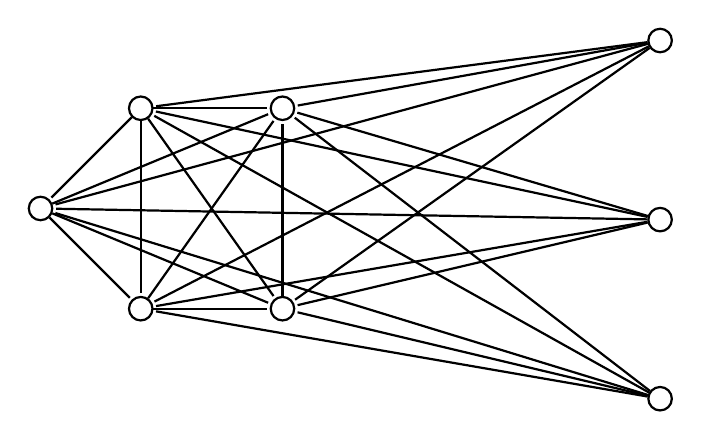
\begin{tikzpicture}[-,>=stealth,shorten >=1pt,auto,node distance=2cm,thick,main node/.style={scale=0.9,circle,draw,font=\sffamily\normalsize}]
            \node[main node] (1) {};
            \node[main node] (2) [below left of=1] {};
            \node[main node] (3) [below right of=2] {};
            \node[main node] (6) [right of=1] {};
            \node[] (5) [below right of=6] {};
            \node[main node] (4) [right of=3] {};

            \node[main node] (7) [right of=5, xshift=50] {};
            \node[main node] (8) [above of=7, yshift=15] {};
            \node[main node] (9) [below of=7, yshift=-15] {};

            \path[every node/.style={font=\sffamily\small}]
                (1) edge (2)
                (1) edge (3)
                (1) edge (4)
                (1) edge (6)

                (2) edge (3)
                (2) edge (4)
                (2) edge (6)

                (3) edge (4)
                (3) edge (6)

                (4) edge (6)

                (7) edge (1)
                (7) edge (2)
                (7) edge (3)
                (7) edge (4)
                (7) edge (6)

                (8) edge (1)
                (8) edge (2)
                (8) edge (3)
                (8) edge (4)
                (8) edge (6)

                (9) edge (1)
                (9) edge (2)
                (9) edge (3)
                (9) edge (4)
                (9) edge (6)
                ;
        \end{tikzpicture}

        \caption{The complete split graph with a $5$-clique and an independent set of $3$ vertices}
    \end{figure}

    Any complete split graph with a $(k-1)$-clique and an independent set of $n-(k-1)$ vertices has as edge count:
    \[\abs{E(G)} = (k-1)(n-(k-1)) + \binom{k-1}{2}\]

    Moreover, such split graphs are clearly not $k$-connected since removing the $(k-1)$-cliques disconnects it, implying that $c_k \geq k-1$.
    
    \section{Existence of cliques as minors}

    In \Cref{topmin} we introduced the concept of topological minor through subdivisions. In this section, we give a more general definition of the concept of \textbf{minors}, a fundamental structure studied in graph theory.

    Consider a graph $G$ and an edge $xy \in E(G)$. A \tbf{contraction} of $xy$ on $G$ refers to the process of merging the two vertices $x$ and $y$ into a new vertex $z$, moving all the edges of $x$ and $y$ to $z$ and deleting any \textbf{parralel edge} (or \textit{multi-edges}) that formed during the process. The contacted graph is denoted with $G/xy$.

    \begin{figure}[H]
        \centering
        \begin{tabular}{ccc}
            \begin{tabular}{c}
                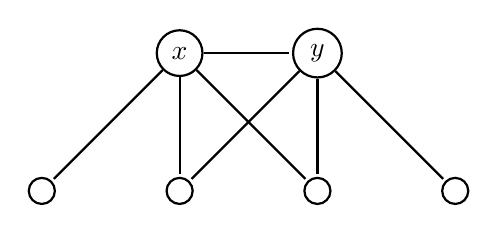
\begin{tikzpicture}[-,>=stealth,shorten >=1pt,auto,node distance=1.75cm, thick,main node/.style={scale=0.9,circle,draw,font=\sffamily\normalsize}]
        
                    \node[circle, draw] (1) []{$x$};
                    \node[circle, draw] (2) [right of = 1]{$y$};
                    \node[circle, draw] (4) [below of = 1]{};
                    \node[circle, draw] (3) [left of = 4]{};
                    \node[circle, draw] (5) [below of = 2]{};
                    \node[circle, draw] (6) [right of = 5]{};
        
                    \draw[-] (1) to (2);
                    \draw[-] (1) to (3);
                    \draw[-] (1) to (4);
                    \draw[-] (1) to (5);
                    \draw[-] (2) to (4);
                    \draw[-] (2) to (5);
                    \draw[-] (2) to (6);
        
                    ;
                \end{tikzpicture}
            \end{tabular}

            &\quad$\implies$\quad &

            \begin{tabular}{c}
                
                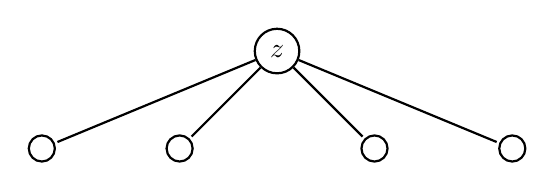
\begin{tikzpicture}[-,>=stealth,shorten >=1pt,auto,node distance=1.75cm, thick,main node/.style={scale=0.9,circle,draw,font=\sffamily\normalsize}]

                    \node[circle, draw] (1) []{$z$};
                    \node[circle, draw] (2) [below left of = 1]{};
                    \node[circle, draw] (3) [left of = 2]{};
                    \node[circle, draw] (4) [below right of = 1]{};
                    \node[circle, draw] (5) [right of = 4]{};

                    \draw[-] (1) to (2);
                    \draw[-] (1) to (3);
                    \draw[-] (1) to (4);
                    \draw[-] (1) to (5);

                    ;
                \end{tikzpicture}
            \end{tabular}
        \end{tabular}
        \caption{Example of edge contraction.}
    \end{figure}

    \begin{frameddefn}{Minor}
        Let $G$ be a graph. A graph $H$ is a \textbf{minor} of $G$ if $H$ can be obtained from $G$ by removing vertices, edges and by contracting edges.
    \end{frameddefn}
    
    \begin{figure}[H]
        \centering
        \begin{tabular}{ccc}
            \begin{tabular}{c}
                \begin{tikzpicture}[-,>=stealth,shorten >=1pt,auto,node distance=1.5cm, thick,main node/.style={scale=0.9,circle,draw,font=\sffamily\normalsize}]

                    \node[circle, draw] (1) []{};
                    \node[circle, draw] (2) [right of = 1]{};
                    \node[circle, draw] (3) [right of = 2]{};
                    \node[circle, draw] (4) [right of = 3]{};
                    \node[circle, draw, dashed] (5) [right of = 4]{};
                    \node[circle, draw] (6) [above of = 2]{};
                    \node[circle, draw] (7) [below of = 3]{};

                    \draw[-] (1) to (2);
                    \draw[dashed] (1) to (6);
                    \draw[-] (2) [color = Carmine, line width = 2] to (3);
                    \draw[-] (3) to (4);
                    \draw[dashed] (4) to (5);
                    \draw[-] (2) to (6);
                    \draw[-] (3) to (7);
                    \draw[dashed] (4) to (7);

                    ;
                \end{tikzpicture}
            \end{tabular}

            &\quad$\implies$\quad&

            \begin{tabular}{c}
                \begin{tikzpicture}[-,>=stealth,shorten >=1pt,auto,node distance=1.5cm, thick,main node/.style={scale=0.9,circle,draw,font=\sffamily\normalsize}]

                    \node[circle, draw] (1) []{};
                    \node[circle, draw] (x) [right of = 1]{};
                    \node[circle, draw] (4) [right of = x]{};
                    \node[circle, draw] (6) [above of = 2]{};
                    \node[circle, draw] (7) [below of = x]{};

                    \draw[-] (1) to (2);
                    \draw[-] (x) to (4);
                    \draw[-] (2) to (6);
                    \draw[-] (x) to (7);
                    ;
                \end{tikzpicture}
            \end{tabular}
        \end{tabular}

        \caption{By removing the dashed edges and vertices and contracting the red edge, we get the cross graph as a minor}
    \end{figure}

    It's easy to see that topological minors are minors. Consider a graph $G$ that has $H$ as topological minor, meaning that it contains a graph $H'$ that is a subdivision of $H$. If we remove from $G$ all the edges and vertices that are not part of $H'$, we are left with a subdivision of $H$. Through edge contraction, each edge subdivision can be reversed, obtaining $H$ as a minor. This allows us to form some sort of \textbf{structure hierarchy} in graphs.
    \[H \text{ ind. subgraph of } G \implies H \text{ subgraph of } G \implies H \text{ top. minor of } of G \implies H \text{ minor of } G\]

    It's easy to see that the first three levels of this hierarchy are strict inclusions, i.e. not all subgraphs are induced and not all topological minors are subgraphs. The same also holds for the last level of the hierarchy. For instance, consider the following graph.

    \begin{figure}[H]
        \centering
        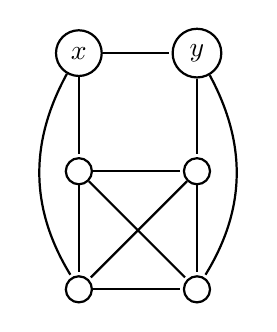
\begin{tikzpicture}[-,>=stealth,shorten >=1pt,auto,node distance=1.5cm, thick,main node/.style={scale=0.9,circle,draw,font=\sffamily\normalsize}]

            \node[circle, draw] (1) []{$x$};
            \node[circle, draw] (2) [right of = 1]{$y$};
            \node[circle, draw] (3) [below of = 1]{};
            \node[circle, draw] (4) [below of = 2]{};
            \node[circle, draw] (5) [below of = 3]{};
            \node[circle, draw] (6) [below of = 4]{};

            \draw[-] (1) to (2);
            \draw[-] (1) to (3);
            \draw[-] (1) [bend right] to (5);
            \draw[-] (2) to (4);
            \draw[-] (2) [bend left] to (6);
            \draw[-] (3) to (4);
            \draw[-] (3) to (5);
            \draw[-] (3) to (6);
            \draw[-] (4) to (5);
            \draw[-] (4) to (6);
            \draw[-] (5) to (6);

            ;
        \end{tikzpicture}
    \end{figure}

    If we contract the edge $xy$, we obtain $K_5$ as a minor. However, $K_5$ is not a topological minor of $G$: every subdivision of $K_5$ has at least 5 vertices of degree 4, but $G$ has only 4 vertices of degree 4. 

    \newpage

    \begin{framedthm}[label={extr_kp_minor}]{Extremal conditions for $k$-cliques as minors}
        Let $p$ be an integer $2 \le p \le 7$. If $G$ is a graph such that $\abs{E(G)} \ge (p - 2)n - \binom{p - 1}{2} + 1$ then $G$ contains $K_p$ as minor.
    \end{framedthm}

    \begin{proof}
        The theorem is proved individually for each value of $p$.
        \begin{itemize}
            \item For $p = 2$, we have that:
            \[\abs{E(G)} \ge (2 - 2)n - \binom{2 - 1}{2} + 1 = 1\]
            Since a single edge corresponds to $K_2$, we conclude that $G$ contains $K_2$ as a subgraph and hence as a minor.
            
            \item For $p = 3$, we have that:
            \[\abs{E(G)} \ge (3 - 2)n - \binom{3 - 1}{2} + 1 = n-1+1 = n\]
            Since a forest has at most $n-1$ edges, we get that $G$ must contain at least a cycle. This cycle can be contracted into $K_3$, concluding that $G$ contains $K_3$ as a minor.

            \item For $p = 4$, we have that:
            \[\abs{E(G)} \ge (4 - 2)n - \binom{4 - 1}{2} + 1 = 2n-3+1 = 2n-2\]

            We proceed by induction on $n+m$. We observe that if $n = 3$ then $\abs{E(G)} \ge 2 \cdot 3 - 2 = 4$ which is impossible with only 3 vertices. Hence, to satisfy the edge bound $n$ must be at least 4. Therefore, for the base case assume that $n = 4$, which means that 
            \[\abs{E(G)} \ge 2 \cdot 4 - 2 = 6 = \binom{4}{2}\]
            
            concluding that $G = K_4$, thus it contains itself as a minor. Assume the inductive hypothesis and consider the case $n+m+1$. Suppose that $\abs{E(G)} > 2n-2$. Then, for any edge $e \in E(G)$ it holds that $\abs{E(G-e)} \geq 2n-2$. By inductive hypothesis, we conclude that $G-e$ contains $K_4$ as a minor, hence $G$ also does.

            Consider now the case where $\abs{E(G)} = 2n-2$. Then, for any edge $e \in E(G)$ we have that $G/e$ has $n-1$ vertices. Again, if $\abs{E(G/e)} \geq 2(n-1)-2$ then by inductive hypothesis $G/e$ contains $K_4$ as a minor, hence $G$ also does. Therefore, we may assume that $\abs{E(G)} = 2n-2$ and that $\abs{E(G/e)} < 2(n-1)-2$ for all $e \in E(G)$.
            
            \textbf{Claim 1}: every edge $e \in E(G)$ is contained inside two distinct 3-cliques.

            \begin{proof}[Proof of Claim 1]
                Fix an edge $e \in E(G)$. Since $\abs{E(G)} = 2n-2$ and $\abs{E(G/e)} < 2(n-1)-2$, at least 3 edges must have been deleted during the contraction. One of those edges is clearly the edge $e$, while the other two must be parallel edges that have been removed afterwards. However, this can happen only if the edge $e$ is contained inside two distinct 3-cliques (see \Cref{double_triangle}). By applying the same reasoning on all edges, we conclude the claim.
            \end{proof}

            Since every edge of $G$ is contained inside two 3-cliques, we get that $\delta(G) \geq 3$. By way of contradiction, suppose that $\delta(G) \geq 4$. Then, by the Handshaking lemma we get that:
            \[\abs{E(G)} \geq \frac{4}{2}n = 2n\]
            contradicting the assumption for which $\abs{E(G)} = 2n-2$. Thus, we get that $\delta(G) = 3$, implying that there is at least one vertex $v \in V(G)$ such that $\deg(v) = 3$.

            \textbf{Claim 2}: $N(v) \cup \{v\} = K_4$

            \begin{proof}[Proof of Claim 2]
                By way of contradiction, suppose that there are two vertices $x,y \in N(v)$ such that $xy \notin E(G)$. By Claim 1, the edge $vx$ must be contained inside two distinct 3-cliques. However, since $xy \notin E(G)$, these two cliques cannot contain both $x$ and $y$. Without loss of generality, suppose that one of the first cliques is formed by the vertices $\{v,x,z\}$, where $z$ is the third neighbor of $v$. Then, in order to form the second clique, there must be another vertex $w$ in order to form the clique $\{v,x,w\}$, contradicting the fact that $\deg(v) = 3$. This concludes that for all $x,y \in N(V)$ it holds that $x \sim y$, forming a 3-clique. By adding the three edges connecting $v$ to $N(v)$, we get a 4-clique.
            \end{proof}

            Since $v$ and its neighborhood form a $K_4$ clique, we conclude that $G$ contains $K_4$ as a minor.

            \item For $p = 5$, we have that:
            \[\abs{E(G)} \ge (5 - 2)n - \binom{5 - 1}{2} + 1 = 3n-6+1 = 3n-5\]

            We proceed by induction on $n+m$. We observe that if $n = 3$ then $\abs{E(G)} \ge 3 \cdot 3 - 5 = 4$ which is impossible with only 3 vertices. The same goes for the case $n = 4$. Hence, to satisfy the edge bound $n$ must be at least $5$. Therefore, for the base case assume that $n = 5$, which means that 
            \[\abs{E(G)} \ge 3 \cdot 5 - 5 = 10 = \binom{5}{2}\]

            concluding that $G = K_5$, thus it contains itself as a minor. Assume the inductive hypothesis and consider the case $n+m+1$. Suppose that $\abs{E(G)} > 3n-5$. Then, for any edge $e \in E(G)$ it holds that $\abs{E(G-e)} \geq 3n-5$. By inductive hypothesis, we conclude that $G-e$ contains $K_5$ as a minor, hence $G$ also does.

            Consider now the case where $\abs{E(G)} = 3n-5$. Then, for any edge $e \in E(G)$ we have that $G/e$ has $n-1$ vertices. Again, if $\abs{E(G/e)} \geq 3(n-1)-5$ then by inductive hypothesis $G/e$ contains $K_4$ as a minor, hence $G$ also does. Therefore, we may assume that $\abs{E(G)} = 3n-5$ and that $\abs{E(G/e)} < 3(n-1)-5$ for all $e \in E(G)$.
            
            Through the same reasoning as Claim 1 of the case $p = 4$, we get that every edge $e \in E(G)$ is contained inside three distinct 3-cliques. Since every edge of $G$ is contained inside three 3-cliques, we get that $\delta(G) \geq 4$. By way of contradiction, suppose that $\delta(G) \geq 6$. Then, by the Handshaking lemma we get that:
            \[\abs{E(G)} \geq \frac{6}{2}n = 3n\]
            contradicting the assumption for which $\abs{E(G)} = 3n-5$. Thus, we get that $\delta(G) \leq 5$. Let $v$ a vertex of minimum degree in $G$, implying that $\deg(v) \in \{4,5\}$. We have two sub-cases:
            \begin{enumerate}
                \item $\deg(v) = 4$. Through the same reasoning as Claim 2 of the case $p = 5$ we conclude that $N(v) \cup \{v\} = K_5$.
                \item $\deg(v) = 5$. Unlike the above case, we cannot directly conclude that $v$ and its neighborhood form a $5$-clique since in this case we have a total of 6 edges. However, the same reasoning still allows us to deduce that $\delta(G[N(v)]) \geq 3$ and that $\Delta(G[N(v)]) \leq 4$.
                
                If $\delta(G[N(v)]) = 4$ then $G[N(v)] = K_5$, concluding the proof. Hence, we may assume that $\delta(G[N(v)]) = 3$. Since $\abs{N(v)} = 5$, the Handshaking lemma gurantees that at least one neighbor of $v$ has degree 4, since otherwise we would have an odd number of odd-degree vertices, which is impossible. This implies that $N(v)$ is missing either 1 or 2 edges from being a 5-clique.
                
                If there is only one \textit{anti-edge}, that being a missing edge, contracting any of the edges $xy$ adjacent to it will induce that $G[N(v)] / xy = K_4$, hence $G[N(v) \cup {v}] / xy = K_5$. Otherwise, if there are two anti-edges, contracting any of the edges $zw$ that are adjacent to both of them will induce that $G[N(v)] / zw = K_4$, hence $G[N(v) \cup {v}] / zw = K_5$.
            \end{enumerate}

            \item For $p=6$ and $p=7$, the proof is similar to $p = 4$ and $p = 5$
        \end{itemize}
    \end{proof}

    \begin{figure}[H]
        \centering

        \begin{tabular}{c}
            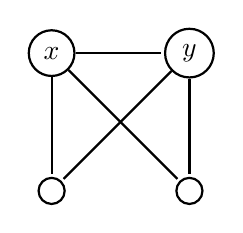
\begin{tikzpicture}[-,>=stealth,shorten >=1pt,auto,node distance=1.75cm, thick,main node/.style={scale=0.9,circle,draw,font=\sffamily\normalsize}]
    
                \node[circle, draw] (1) []{$x$};
                \node[circle, draw] (2) [right of = 1]{$y$};
                \node[circle, draw] (4) [below of = 1]{};
                \node[circle, draw] (5) [below of = 2]{};
    
                \draw[-] (1) to (2);
                \draw[-] (1) to (4);
                \draw[-] (1) to (5);
                \draw[-] (2) to (4);
                \draw[-] (2) to (5);
    
                ;
            \end{tikzpicture}
        \end{tabular}

        \caption{The two 3-cliques containing the edge $e$ in the case $p=4$ of the previous proof.}
        \label{double_triangle}
    \end{figure}

    The cases with $p \in \{2,3,4,5\}$ were first proven by \textcite{dirac} and later independently by \textcite{gyori}, while the cases $p \in \{6,7\}$ were proven by \textcite{mader}. \textcite{jorgensen} proved that the theorem also extends to $p = 8$, with the exception of an infinite family of graphs for which it doesn't hold. Similarly, \textcite{song} proved that the theorem extends to $p = 9$ with the exception of two infinite families of graphs, while \textcite{zhu} proved that for $p = 10$ the theorem holds except for a few infinite families. Both of the latter results were proven with the assistance of a computer.

    In a series of papers, \textcite{kostochaka, thomason} were able to prove the existence of a constant for which the theorem holds in every graph, with a different edge bound. This theorem can be seen as a generalization of theorem \Cref{boll_thom}. Thomason also proved that this bound is optimal since there are some \textit{Erdős-Rényi random graphs} that have $c' p \sqrt{\log p} n$ edges and no $K_p$ minor, where $c'< c$. Interestingly, for these graphs it also holds that $n$ is in function of $p$.

    \begin{framedthm}{Kostochaka-Thomason theorem}
        There is a constant $c > 0$ such that any graph $G$ with $\abs{E(G)} \geq cp \sqrt{\log p} n$ contains $K_p$ as a minor.
    \end{framedthm}

    \begin{proof}
        Omitted.
    \end{proof}

    Seymour and Thomas conjectured that the missing condition for \Cref{extr_kp_minor} to hold for every $p \geq 2$ is the $(p-2)$-connectivity of the graph.
    
    \begin{framedconj}{Seymour-Thomas conjecture}
        For all $p \in \N$ there is a constant $N_p > 0$ such that any $(p-2)$-connected graph $G$ with $n \geq N_p$ and $\abs{E(G)} \geq (p-2)n-\binom{p-1}{2}+1$ contains $K_p$ as a minor.
    \end{framedconj}

    The closest result for this conjecture was proven by \textcite{bohme}.

    \begin{framedthm}{Linear connectivity and clique minors}
        There is a constant $c > 0$ such that for all $p \in \N$ there is another constant $N_p > 0$ for which any $c(p+1)$-connected graph $G$ with $n \geq N_p$ contains $K_p$ as a minor.
    \end{framedthm}

    \begin{proof}
        Omitted.
    \end{proof}

    
    \section{Ramsey numbers}

    In previous sections we focused on finding extremal number of edges that guarantee the presence of some structure inside a graph. In this section, we'll discuss extremal number of nodes. In particular, we focus on the minimal number of nodes that force a graph to contain either a \textit{$t$-clique} or a \textit{$t$-indset}, i.e. an independent set of $t$ nodes. This extremal number of nodes is known in the literature as \textbf{Ramsey number}, named after F. P. Ramsey, the pioneer and main researcher of this problem. Ramsey numbers are of fundamental interest in graph theory due to being one of the hardest question in the whole field.

    \begin{frameddefn}{Ramsey number}
        Given $t \in \N$, we define the \textbf{Ramsey number} $R(t)$ as the minimum value such that all graphs with at least $R(t)$ nodes contain a $t$-clique or a $t$-indset.
    \end{frameddefn}

    It's easy to see that $R(1) = 1$ and $R(2) = 2$ since a single vertex is both a $1$-clique and a $1$-indset and two vertices can be either a $2$-clique or a $2$-indset. For the value $R(3)$, instead, by definition we have that $R(3) \geq 3$ since otherwise we could never have a $3$-clique or a $3$-indset. Moreover, we can also prove that $R(3) > 5$ since we can find graphs with 3, 4 and 5 vertices that don't contain neither a $3$-clique nor a $3$-indset.

    \begin{figure}[H]
        \centering
        \resizebox{0.6\textwidth}{!}{
            \begin{tikzpicture}[-, >=stealth, shorten >= 1pt, auto, node distance=2cm, thick, main node/.style={scale=3,circle,draw,font=\sffamily\normalsize}]
                \node[main node] (1) {};
                \node[main node] (2) [below left of = 1]{};
                \node[main node] (3) [below right of = 2]{};

                \node[main node] (4) [right of = 1, xshift = 50]{};
                \node[main node] (5) [right of = 3, xshift = 50]{};
                \node[main node] (6) [right of = 4]{};
                \node[main node] (7) [right of = 5]{};

                \node[] (x) [right of = 2, xshift = 1000]{};
                \node[main node] (8) [above of = x] {};
                \node[main node] (9) [right of = x, yshift=15]{};
                \node[main node] (10) [below right of = x]{};
                \node[main node] (11) [below left of = x]{};
                \node[main node] (12) [left of = x, yshift=15]{};

                \path[every node/.style={font=\sffamily\small}]
                    (1) edge (2)

                    (4) edge (5)
                    (6) edge (7)

                    (8) edge (9)
                    (9) edge (10)
                    (10) edge (11)
                    (11) edge (12)
                    (12) edge (8)
                ;
            \end{tikzpicture}
        }

        \caption{The three graphs with 3 (left), 4 (middle) and 5 (right) vertices giving the $R(3) > 5$ lower bound.}
    \end{figure}

    We observe that this lower bound is actually tight, meaning that $R(3) = 6$.

    \begin{framedprop}[label={ramsey_3}]{}
        $R(3) = 6$
    \end{framedprop}

    \begin{proof}
        Through the previous counter examples we know that $R(3) \geq 6$, hence it suffices to prove that $R(3) \leq 6$.
        
        Since every graph with more than $6$ vertices contains a subgraph with $6$ vertices, we can restrict our focus on graphs with $6$ vertices. Let $G$ be one such graph. By way of contradiction, suppose that $G$ contains neither a $3$-clique nor a $3$-indset.

        \textbf{Claim}: $\Delta \leq 2$

        \begin{proof}[Proof of the claim.]
            Fix a vertex $v \in V(G)$. Each pair of vertices $x,y \in N(v)$ must be non-adjacent, since otherwise $v,x,y$ form a $3$-clique, raising a contradiction. Hence, $N(x)$ must be an independent set, implying that $\abs{N(x)} < 3$ since otherwise $G$ contains a $3$-indset.
        \end{proof}

        Fix a vertex $u \in V(G)$. By the claim, we know that $\abs{N(u)} < 3$, thus $\abs{\overline{N(u) \cup \{u\}}} = 6-\abs{N(u) \cup \{u\}} \geq 3$. We have two cases:
        \begin{enumerate}
            \item $\exists x,y \in \overline{N(u)\cup \{u\}}$ such that $x \not\sim y$. Then, $u,x,y$ form a $3$-indset.
            \item $\forall x,y \in \overline{N(u)\cup \{u\}}$ it holds that $x \sim y$. Then, $\overline{N(u)\cup \{u\}}$ contains a $3$-clique.
        \end{enumerate}

        In both cases, the initial assumption is contradicted.
    \end{proof}

    For the case $t = 4$, \textcite{r4_lower_bound} proved the lower bound $R(4) > 17$ through a graph with $17$ vertices that contains neither a $4$-clique nor a $4$-indset. This graph uses $Z_17$ as vertex set, meaning that $V(G) = \{x_0, \ldots, x_{16}\}$, where $x_ix_j \in E(G)$ if and only if $i-j \equiv \pm 2^i \pmod{17}$, with $0 \leq i \leq 3$.

    \begin{figure}[H]
        \centering
        \includegraphics[scale=0.5]{images/r4_lb.png}

        \caption{Kalbfleisch's graph giving the $R(4) >17$ lower bound.}
        \label{r4_lb}
    \end{figure}

    Again, this lower bound can be shown to be tight. To achieve this result, we first give a generalization of the Ramsey number.

    \begin{frameddefn}{Complementary graph}
        Given a graph $G$, we define the \textbf{complementary graph} as the graph $\overline{G}$ such that $V(\overline{G}) = V(G)$ and $E(\overline{G}) = \overline{E(G)}$.
    \end{frameddefn}


    \begin{figure}[H]
        \centering
        \resizebox{0.6\textwidth}{!}{
            \begin{tikzpicture}[-, >=stealth, shorten >= 1pt, auto, node distance=2cm, thick, main node/.style={scale=3,circle,draw,font=\sffamily\normalsize}]
                \node[] (x) []{};
                \node[main node] (8) [above of = x] {};
                \node[main node] (9) [right of = x, yshift=15]{};
                \node[main node] (10) [below right of = x]{};
                \node[main node] (11) [below left of = x]{};
                \node[main node] (12) [left of = x, yshift=15]{};

                \node[] (y) [right of = x, xshift = 500]{};
                \node[main node] (1) [above of = y] {};
                \node[main node] (2) [right of = y, yshift=15]{};
                \node[main node] (3) [below right of = y]{};
                \node[main node] (4) [below left of = y]{};
                \node[main node] (5) [left of = y, yshift=15]{};
                
                \path[every node/.style={font=\sffamily\small}]
                    (8) edge (9)
                    (9) edge (10)
                    (10) edge (11)
                    (11) edge (12)
                    (12) edge (8)

                    (1) edge (3)
                    (1) edge (4)

                    (2) edge (4)
                    (2) edge (5)

                    (3) edge (5)
                ;
            \end{tikzpicture}
        }

        \caption{The cycle $C_5$ and the graph $\overline{C_5}$}
    \end{figure}

    It's easy to see that, by definition, the complement of a complementary graph is equal to the former graph, i.e. $\overline{\overline{G}} = G$. Moreover, any $t$-clique in $G$ corresponds to a $t$-indset in $\overline{G}$. This allows to reformulate the definition of $R(t)$: it is the minimal value such that one between $G$ and $\overline{G}$ contains a $t$-clique. We now give a more general formulation of the Ramsey number.

    \begin{frameddefn}{Generalized Ramsey number}
        Given $s,t \in \N$, we define the \textbf{Generalized Ramsey number} $R(s,t)$ as the minimum value such that for all graphs $G$ with at least $R(s,t)$ vertices it holds that $G$ contains an $s$-clique or $\overline{G}$ contains a $t$-clique.
    \end{frameddefn}

    By definition, we have that $R(t) = R(t,t)$. Moreover, through the previous observations, we get that $R(s,t) = R(t,s)$. This symmetry of the general Ramsey number can be used to easily derive upper bounds.

    \begin{framedlem}{}
        For any $t \in \N$, it holds that $R(t) \leq 2R(t, t-1)$.
    \end{framedlem}

    \begin{proof}
        Let $k = R(t, t-1)$ and let $G$ be a graph with $n = 2k$ nodes. Given any vertex $v \in V(G)$, we observe that $v$ has either at least $k$ neighbors or at least $k$ non-neighbors, i.e. either $\abs{N(v)} \geq k$ or $\abs{\overline{N(v) \cup \{v\}}} \geq k$. We recall that $k = R(t,t-1) = R(t-1,t)$. Then, in the first case we get that $N(v)$ contains a $(t-1)$-clique or a $t$-indset, thus that $N(v) \cup \{v\}$ contains a $t$-clique or a $t$-indset. In the second case, instead, we get that $\overline{N(v) \cup \{v\}}$ contains a $t$-clique or a $(t-1)$-indset, thus that $\overline{N(v)}$ contains a $t$-clique or a $t$-indset.
    \end{proof}

    \begin{framedprop}{}
        $R(4,3) \leq 9$
    \end{framedprop}

    \begin{proof}
        Since every graph with more than $9$ vertices contains a subgraph with $9$ vertices, we can restrict our focus on graphs with $9$ vertices. Let $G$ be one such graph. By way of contradiction, suppose that $G$ contains neither a $4$-clique nor a $3$-indset.

        \textbf{Claim 1}: $\Delta \leq 5$.

        \begin{proof}[Proof of Claim 1]
            Fix a vertex $v \in V(G)$. By way of contradiction, suppose that $\abs{N(v)} \geq 6$. Then, by \Cref{ramsey_3} $N(v)$ contains a $3$-clique or a $3$-indset. In the first case, we get that $N(v) \cup v$ contains a $4$-clique, thus $G$ also does. In the second case, $N(v)$ contains a $3$-indset, thus $G$ also does. Both cases raise a contradiction.
        \end{proof}

        \textbf{Claim 2}: $\delta \geq 5$

        \begin{proof}[Proof of Claim 2]
            Fix a vertex $v \in V(G)$. By way of contradiction, suppose that $\abs{N(v)} \leq 4$. Then, we have that $\abs{\overline{N(v) \cup \{v\}}} = 9 - \abs{N(v) \cup \{v\}} \geq 4$. We have two cases:
            \begin{enumerate}
                \item $\exists x,y \in \overline{N(u)\cup \{u\}}$ such that $x \not\sim y$. Then, $u,x,y$ form a $3$-indset.
                \item $\forall x,y \in \overline{N(u)\cup \{u\}}$ it holds that $x \sim y$. Then, $\overline{N(u)\cup \{u\}}$ contains a $4$-clique.
            \end{enumerate}
    
            In both cases, the initial assumption is contradicted.
        \end{proof}

        Since $\delta = \Delta = 5$, we get that $5$ is 5-regular. However, by the Handshaking lemma, there cannot be an odd-regular graph with an odd number of vertices:
        \[2 \abs{E(G)} = \sum_{v \in V(G)} \deg(v) = 5\cdot 9 = 45\]
        
        This concludes that such graph $G$ cannot exist.
    \end{proof}

    \begin{framedcor}{}
        $R(4) = 18$
    \end{framedcor}

    \begin{proof}
        Follows from the above lemma, the above proposition and the lower bound given in \Cref{r4_lb}
    \end{proof}

    Using ideas similar to the above proposition, one can prove that $R(5,4) \leq 25$, which immediately gives the upper bound $R(5) \leq 50$. However, this upper bound is not always tight. In fact, very recenlty \textcite{angeltveit} proved that $R(5) \leq 46$. Moreover,  also known that $R(5) \geq 43$ \textcite{exoo}. Even though $R(5)$ lies between these 4 values, finding the actual value is still a very hard task. In particular, this task is even hard to reach with computer assisted proofs (there are at least $2^{\binom{43}{2}} = 2^{903}$ graphs to analyze).

    For $R(6)$, the current known bounds are $102 \leq R(6) \leq 160$. To give an intuition behind the hardness of this problem, Paul Erdős said the following: \curlyquotes{imagine an alien force, vastly more powerful than us, landing on Earth and demanding the value of $R(5)$ or they will destroy our planet. In that case, we should marshal all our computers and all our mathematicians and attempt to find the value. If instead they ask for the value of $R(6)$, we should attempt to destroy the aliens.}

    What about the general case? Can we even be sure that $R(t)$ exists for every value of $t$? This question was positively answered by \textcite{ramsey} in the paper that gave birth to this field of graph theory.

    \begin{framedthm}{Ramsey's theorem}
        For any $t \in \N$, the value $R(t)$ exists and is bounded by $R(t) \leq 2^{2t-3}$ when $t \geq 2$.
    \end{framedthm}

    \begin{proof}
        We already know that $R(1)= 1$ and $R(2) = 2$, hence they exist. Fix $t \in \N$ with $t \geq 2$ and let $G$ be a graph with $2^{2t-3}$ nodes.
        
        \textbf{Claim:} there is a sequence of sets $X_1, \ldots, X_{2t-3}$ and vertices $x_1, \ldots, x_{2t-3}$ such that for each $i \in [2t-2]$ it holds that:
        \begin{enumerate}
            \item $x_i \in X_i$ and $\abs{X_i} \geq 2^{2t-2-i}$
            \item $X_{i+1} \subseteq X_i - \{x_i\}$
            \item $x_i$ is either adjacent to every vertex of $X_{i+1}$ or non-adjacent to all vertices of $X_{i+1}$
        \end{enumerate}

        \begin{proof}
            We construct the sequences in an inductive way. For $i = 1$, we set $X_1 = V(G)$ and choose $x_1$ as any vertex of the graph. The set $X_2$ is then given by the largest set among $N(x_1)$ and $\overline{N(x_1) \cup \{x_1\}}$. By construction, the two last properties are satisfied. For the first property, we observe that:
            \[N(x-1) \cup (\overline{N(x_1) \cup \{x_1\}}) = X_1 - \{x_1\}\]
    
            thus:
            \[\max (N(x_1), \overline{N(x_1) \cup \{x_1\}}) \geq \ceil{\frac{2^{2t-3}-1}{2}} \geq 2^{2t-2-1}\]

            Assume now that the sequence is defined up to some $i < 2t-2$. The set $X_{i+1}$ is then given by the largest set among $N(x_i) \cap X_i$ and $(\overline{N(x_i) \cup \{x_i\}}) \cap X_i$. Again, the two last properties are satisfied by construction of $X_{i+1}$. For the first property, we observe that:
            \[(N(x_i) \cap X_i) \cup ((\overline{N(x_i) \cup \{x_i\}}) \cap X_i) = X_i- \{x_i\}\]
    
            thus:
            \[\max (N(x_i) \cap X_i, (\overline{N(x_i) \cup \{x_i\}}) \cap X_i) \geq \ceil{\frac{2^{2t-2-i}-1}{2}} = 2^{2t-2-(i+1)}\]
        \end{proof}

        \textbf{Claim}: for each $i,j \in [2t-2]$ such that $i < j$ it holds that:
        \begin{itemize}
            \item If $x_i \sim x_j$ then $x_i \sim x_{j'}$ for all $j' \in [i+1, 2t-2]$
            \item If $x_i \not\sim x_j$ then $x_i \not\sim x_{j'}$ for all $j' \in [i+1, 2t-2]$
        \end{itemize}

        \begin{proof}
            Given any $j' \in [i+1, 2t-2]$, by construction of the sequence we have that $x_{j'} \in X_{j'} \subseteq X_{j} \subseteq X_{i+1}$. Hence, by construction of $X_{i+1}$, we know that $x_i$ is either adjacent to all the vertices in $X_{i+1}$ or non-adjacent to all of them. Thus, since $j \in [i+1, 2t-2]$ also holds, if $x_i \sim x_j$ then $x_i \sim x_{j'}$, otherwise $x_i \not\sim x_{j'}$.
        \end{proof}

        Consider now the set $K = N(x_{2t-2}) \cap \{x_1, \ldots, x_{2t-2}\}$. If $\abs{K} \geq t-1$ then the Claim 2 ensures that $K \cup \{x_{2t-2}\}$ contains a clique of size $t$. $\abs{K} \leq t-2$, instead, by Claim 2 $\overline{N(x_{2t-2})}$ contains an independent set of size $2t-2-\abs{K} \geq 2t-2-(t-2) = t$.
    \end{proof}

    Ramsey's theorem gives the upper bound $R(t) \leq 2^{2t-3} = \frac{4^t}{8}$. \textcite{erdos_ramsey} gave an asymptotic lower and upper bound on the problem:
    \[\sqrt{2^t} \sim (1+o(1)) \frac{t}{\sqrt{2} e} 2^{\frac{t}{2}}\leq R(t) \leq (1+o(1)) \frac{4^{t-1}}{\sqrt{\pi t}} \sim 4^t\]

    \newpage

    \section{Solved exercises}

    \begin{framedprob}{}
        Let $\mathrm{ex}(n,H)$ be the minimal value such that for every graph $G$ with at least $n$ vertices and at least $\mathrm{ex}(n,H)$ edges it holds that $G$ contains $H$ as a subgraph.
        \begin{enumerate}
            \item Prove that $\mathrm{ex}(n, K_{1,3}) = n+1$
            \item For all $t \geq 4$, find the value $\mathrm{ex}(n, K_{1,t})$ and prove its correctness
        \end{enumerate}
    \end{framedprob}

    \begin{proof}[Solution]
        First, we observe that $G$ contains $K_{1,t}$ as a subgraph if and only if $G$ has a vertex of degree at least $t$. This also implies that $n \geq t+1$ implicitely holds. Then, we also observe that, by the Handshaking lemma, if $\abs{E(G)} = n+1 = \frac{n}{2}(3-1) + 1$ then it's guaranteed that at least one vertex will have degree greater than $2$. Hence, we get that $\mathrm{ex}(n, K_{1,3}) \leq n+1$. Then lower bound $\mathrm{ex}(n, K_{1,3}) > n$, instead, is given by the cycle $C_n$, which has $n$ edges and no vertex of degree at least 3. This concludes that $\mathrm{ex}(n, K_{1,3}) = n+1$. We now generalize the upper bound to any $t \geq 3$.

        \textbf{Claim 1}: for all $t \geq 3$ it holds that $\mathrm{ex}(n, K_{1,t}) \leq \frac{n}{2}(t-1) + 1$.

        \begin{proof}[Proof of Claim 1]
            Fix $t \geq 3$. Let $G$ be any graph such that $\abs{E(G)} \geq \frac{n}{2}(t-1) + 1$. Through some algebraic manipulation we get that:
            \[\begin{split}
                \max_{v \in V(G)} \deg(v) & \geq \avg_{v \in V(G)} \deg(v) \\
                &= \frac{1}{n} \sum_{v \in V(G)} \deg(v) \\
                &= \frac{2\abs{E(G)}}{n} \\
                &= \frac{2}{n} \rbk{\frac{n}{2} (t-1) + 1} \\
                &= t-1 + \frac{2}{n} \\
                &> t-1
            \end{split}\]

            Hence, the vertex with maximum degree has degree at least $t$, concluding that $G$ contains $K_{1,t}$ as a subgraph.
        \end{proof}

        For the lower bound, we generalize the result through an almost complete bipartite graph instead of a cycle. 

        \textbf{Claim 2}: for all $t \geq 3$ it holds that $\mathrm{ex}(n, K_{1,t}) \geq \frac{n}{2}(t-1) + 1$.

        \begin{proof}[Proof of Claim 2]
            Fix $t \geq 3$. Let $G$ be the bipartite graph with bipartition $(X,Y)$ such that $X = \{x_1, \ldots, x_{t-1}\}$, $Y = \{y_1, \ldots, y_{t-1}\}$ and for all $i \in [t-1]$ we have that $N(x_i) = Y-\{y_i\}$ (which also implies that $N(y_i) = X-\{x_i\}$). By construction, every vertex has degree $t-1$, hence $K_{1,t}$ is not a subgraph of $G$. Moreover, given that $n = 2(t-1)$, we have that:
            \[\abs{E(G)} = (t-1)^2 = \frac{2(t-1)}{2}(t-1) = \frac{n}{2}(t-1)\]
            concluding that $\mathrm{ex}(n, K_{1,t}) > \frac{n}{2}(t-1)$
        \end{proof}
    \end{proof}

    \begin{framedprob}{}
        Let $\mathrm{ex}(n,H)$ be the minimal value such that for every graph $G$ with at least $n$ vertices and at least $\mathrm{ex}(n,H)$ edges it holds that $G$ contains $H$ as a subgraph. Find the value of $\mathrm{ex}(n, P_4)$ and prove its correctness.
    \end{framedprob}

    \begin{proof}[Solution]
        The lower bound $\mathrm{ex}(n, P_4) > n$ is easily given by a graph made of two $K_3$ components. We prove that this bound is optimal, i.e. that $\mathrm{ex}(n, P_4) = n+1$. 
        
        Let $G$ be a graph with $\abs{E(G)} \geq n+1$. By way of contradiction, suppose that $G$ doesn't contain $P_4$ as a subgraph. Since any forest graph has $n-1$ edges, we know that $G$ must have at least a component with a cycle. Moreover, we observe that every component containing a cycle must have exactly 3 nodes, otherwise it would contain $P_4$ as a subgraph. Hence, every component of $G$ must be either a 3-clique or a tree. Let $C_1, \ldots, C_k$ be the 3-clique components of $G$ and let $T_1, \ldots, T_h$ be the tree components of $G$. We have that:
        \[\begin{split}
            \abs{E(G)} &= \sum_{i \in [k]} \abs{E(C_i)} + \sum_{j \in [h]} \abs{E(T_j)} \\
            &= 3k + \sum_{j \in [h]} \abs{V(T_j)}-1 \\
            &= 3k + \sum_{j \in [h]} \abs{V(T_j)} - \sum_{j \in [h]} 1 \\
            &= 3k + (n-3k) - h \\
            &= n - h \\
        \end{split}\]

        Since $h \geq 0$, we get that $\abs{E(G)} \leq n$, raising a contradiction. This concludes that $G$ must contain $P_4$ as a subgraph.
    \end{proof}

    \begin{framedprob}{}
        Let $R(H)$ be the minimal value such that for every graph $G$ with at least $R(H)$ vertices it holds that $G$ contains $H$ as a subgraph.
        
        \begin{enumerate}
            \item Find the value of $R(P_4)$ and prove its correctness.
            \item Find the value of $R(P_5)$ and prove its correctness.
            \item Prove a general lower bound for $R(P_n)$ for all $n \in \N$
        \end{enumerate}
    \end{framedprob}

    \begin{proof}

        We start by giving a general lower bound for $P_n$. Let $q = \floor{\frac{n}{2}}-1$ and consider the graph $G = K_{n-1} \cup K_{q}$. It's easy to see that $P_n \not\subseteq G$. Moreover, the complement of $G$ corresponds to $\overline{G} = K_{n-1, q}$, which also doesn't contain $P_n$. Hence, we get that for all $n \in \N$ it holds that $R(P_n) \geq n-1+q+1 = n+\floor{\frac{n}{2}}-1$.

        For the case $n = 4$, we get that $R(P_4) \geq 5$. We now prove that this bound is tight. Let $G$ be a graph with $n = 5$ vertices. Since $G \cup \overline{G} = K_5$ and $\abs{E(K_5)} = \binom{5}{2} = 10$, exactly one between $G$ and $\overline{G}$ has at least $5$ edges. Without loss of generality, let $G$ be such graph. Then, $G$ cannot be a forest since $\abs{E(G)} \geq n$, implying that there is a cycle $C$.

        By way of contradiction, suppose that neither $G$ nor $\overline{G}$ contains $P_4$. Then, we get that $\abs{C} = 3$ since otherwise $P_4 \subseteq C$. Let $C = c_1,c_2,c_3$ and let $V(G-C) = \{x_1,x_2\}$. We observe that $\forall i \in [3]$ it holds that $x_1 \not\sim c_i$ and $x_2 \not\sim c_i$ since otherwise $C \cup {x_1}$ or $C \cup {x_2}$ would contain $P_4$. However, this implies that $\overline{G} = K_{3,2}$, which contains $P_4$, raising a contradiction. Hence, at least one between $G$ and $\overline{G}$ must contain $P_4$.

        For the case $n = 5$, we get that $R(P_5) \geq 6$. We prove that this bound is also tight. Let $G$ be a graph with $n = 6$ vertices. Let $G$ be a graph with $n = 6$ vertices. Since $G \cup \overline{G} = K_6$ and $\abs{E(K_6)} = \binom{6}{2} = 15$, exactly one between $G$ and $\overline{G}$ has at least $8$ edges. Without loss of generality, let $G$ be such graph. Then, $G$ cannot be a forest since $\abs{E(G)} \geq n$, implying that there is a cycle $C$.
        
        By way of contradiction, suppose that neither $G$ nor $\overline{G}$ contains $P_5$. Then, we get that $\abs{C} \leq 4$ since otherwise $P_5 \subseteq C$. Let $X = V(G-C)$. We have two cases:
        \begin{enumerate}
            \item $\abs{C} = 4$. Let $C = c_1, c_2, c_3, c_4$ and let $X = \{x_1,x_2\}$. We observe that none of $x_1$ and $x_2$ can be adjacent to a vertex in $C$, since otherwise we get that $P_5 \subseteq G$. However, this forces that $c_1x_1c_2x_2c_3$ is a $P_5$ anti-path in $\overline{G}$, raising a contradiction.
            
            \item $\abs{C} = 3$. Let $C = c_1, c_2, c_3$ and let $X = \{x_1,x_2,x_3\}$. We observe that it cannot hold that none of the vertices of $X$ are non-adjacent to at least a vertex of $C$ since otherwise $P_5 \subseteq K_{3,3} \subseteq \overline{G}$. Hence, without loss of generality, assume that $x_1 \sim c_1$. Now, for all $i \in \{2,3\}$ it must hold that $x_2 \not\sim c_i$ and $x_3 \not\sim c_i$ since otherwise $P_5 \subseteq G$. This also implies that $x_2 \sim c_1$ and $x_3 \sim c_1$, otherwise $c_2x_2c_1x_3c_3$ is a $P_5$ anti-path in $\overline{G}$. In turn, we get that for all $j \in \{2,3\}$ it must hold that $x_j \not\sim x_1$, otherwise $c_2c_3c_1x_ix_1$ is a $P_5$ path in $G$. However, this forces that $c_2x_2x_1x_3c_3$ is a $P_5$ anti-path in $\overline{G}$, raising a contradiction.
        \end{enumerate}

        In both cases, we get a contradiction, concluding that $P_5$ must exist inside $G$.
    \end{proof}

    \begin{framedprob}{}
        Show that for any choice of the function $c : E(K_{17}) \to \{\mathrm{red}, \mathrm{green}, \mathrm{blue}\}$ there are three vertices $x,y,z \in V(K_{17})$ such that $c(xy) = c(yz) = c(xz)$, i.e. there is a $K_3$ subgraph formed of a single color.
    \end{framedprob}

    \begin{proof}
        Fix a vertex $u \in V(K_{17})$. Since $\deg(u) = 16$, by the Pidgeonhole Principle there must be at least $\ceil{\frac{16}{3}}$ edges $uv_1, \ldots, uv_6$ incident to $v$ sharing the same color. Without loss of generality, suppose that all of these edges are colored in red. We may assume that $\forall i,j \in [6]$ it holds that $c(v_i v_j) \neq \mathrm{red}$, otherwise we get a red triangle. Hence, each edge in the graph $G[X]$ with $X = \{v_1, \ldots, v_6\}$ must be colored either in green or blue. This reduces the problem to finding a $K_3$ subgraph in $G[X]$ that is colored in green or blue, which is equivalent to the Ramsey problem $R(3,3)$. In particular, since $\abs{X} = 6$, we get that $G[X]$ must contain a triangle that is green or blue.
    \end{proof}

    \begin{framedprob}{}
        Let $K$ be the kite graph, i.e. the graph made by two $K_3$ with a common edge. Prove that any graph with at least $\frac{3}{2}n-1$ edges contains $K$ as a minor.
    \end{framedprob}

    \begin{proof}
        We proceed by induction on $n+m$. When $n = 4$, we have that $\abs{E(G)} \geq \frac{3}{2}n-1 = 5$, thus $G$ must contain $K$ as a subgraph. Assume the inductive hypothesis and consider a graph with $n > 4$. If $\abs{E(G)} > \frac{3}{2}n-1$ then for each edge $e \in E(G)$ we have that $\abs{E(G-e)} \geq \frac{3}{2}n-1$, hence by inductive hypothesis $G-e$ contains $K$ as a minor and so does $G$. Hence, we may assume that $\abs{E(G)} = \frac{3}{2}n-1$. Then, we may also assume that there is no edge $e' \in E(G)$ such that $\abs{E(G/e')} \geq \frac{3}{2}(n-1)-1$, otherwise $G/e'$ contains $K$ as a minor by inductive hypothesis. Hence, we have that $\abs{E(G)} = \frac{3}{2}n-1$ and that $\forall e' \in E(G)$ it holds that $\abs{E(G/e')} < \frac{3}{2}(n-1)-1$.
        
        \textbf{Claim 1}: every edge of $G$ lies in a $K_3$
        
        \begin{proof}[Proof of Claim 1]
            Fix an edge $e \in E(G)$. Since $\abs{E(G/e)} < \frac{3}{2}(n-1)-1$, at least two edges get removed during the contraction. However, this can happen if and only if $e$ lies inside a $K_3$ since one edge is the contracted one and the other must be a parallel edge created by the contraction.
        \end{proof}


        \textbf{Claim 2}: if $G$ is disconnected then $G$ contains $K$ as a minor

        \begin{proof}[Proof of Claim 2]
            Let $H_1, \ldots, H_k$ be the components of $G$, with $k \geq 2$. By way of contradiction, suppose that for each $i \in [k]$ it holds that $e(H_i) \leq \frac{3}{2}\abs{H_i} -1$. Then, we have that:
            \[e(G) = \sum_{i = 1}^k e(H_i) \leq \sum_{i = 1}^k (\frac{3}{2} \abs{H_i} - 2) = \frac{3}{2}n - 2k \leq \frac{3}{2}n-4\]
            raising a contradiction. Thus, there must be at least one $H_i$ such that $e(H_i) \geq \frac{3}{2}\abs{H_i} -1$. Then, since $\abs{H_i} \leq n-1$ we conclude that $H_i$ contains $K$ as a minor by inductive hypothesis.
        \end{proof}

        By Claim 2, we may assume that $G$ is connected. Fix an edge $xy \in E(G)$. Let $z \in V(G)$ be the third vertex of a triangle containing the edge $xy$. Consider the graph $G' = G - \{xy, yz, zx\}$. Let $H_1', \ldots, H_t'$ be the components of $G'$.
        
        If $t < 3$ then at least two vertices of $X = \{x,y,z\}$ must be connected by another path $P$, otherwise we would get at least three components for the three vertices. However, this concludes that $G[X] \cup P$ contains $K$ as a minor.

        Suppose now that $t \geq 3$. By way of contradiction, suppose that for each $i \in [k]$ it holds that $e(H_i') \leq \frac{3}{2}\abs{H_i'} - 1$ otherwise $H_i$ contains $K$ as a minor. Then, we have that:
        \[e(G) = 3 + e(G') = 3+ \sum_{i = 1}^t e(H_i') \leq 3 + \sum_{i = 1}^t (\frac{3}{2} \abs{H_i'} - 2) = 3 + \frac{3}{2}n - 2t \leq 3 + \frac{3}{2}n-6 = \frac{3}{2}n - 3\]
        raising a contradiction. Hence, there must be at least one $H_i'$ such that $e(H_i') \geq \frac{3}{2}\abs{H_i'} -1$. Again, since $\abs{H_i} \leq n-1$ we conclude that $H_i'$ contains $K$ as a minor by inductive hypothesis.
    \end{proof}

    
    \chapter{Graph decompositions}

    \section{Block decomposition}

    Graph decompositions are a way to break down a graph into simpler or more structured parts to better understand its properties, make algorithms more efficient, or solve complex problems. Decompositions are also used to characterize some graph properties. We start by discussing \textbf{block decomposition}, used to find the \curlyquotes{weak points} in a graph.    

    \begin{frameddefn}{Block}
        Let $G$ be a graph. A \textbf{block} in $G$ is a maximal conneced subset $H \subseteq G$ without a \textbf{cut vertex}, i.e. a vertex $x$ such that $H-x$ is disconnected.
    \end{frameddefn}

    \begin{figure}[H]
        \centering
        \begin{tikzpicture}[-, >=stealth, shorten >= 1pt, auto, node distance=2cm, thick, main node/.style={scale=0.9,circle,draw,font=\sffamily\normalsize}]

            \node[main node] (1) [] {};

            \node[main node] (2) [below left of = 1] {};
            \node[main node] (3) [below right of = 2] {};
            \node[main node] (4) [left of = 2, xshift=20] {};

            \node[main node] (6) [left of = 4] {};
            \node[main node] (5) [above left of = 6] {};
            \node[main node] (7) [below left of = 6] {};
            
            \path[every node/.style={font=\sffamily\small}]
                (1) edge[color = Green, line width = 2] (2)
                (1) edge[color = Green, line width = 2] (3)
                (2) edge[color = Green, line width = 2] (3)
                (4) edge[color = Green, line width = 2] (1)
                (4) edge[color = Green, line width = 2] (3)

                (4) edge[color = BlueLagoon, line width = 2] (6)

                (5) edge[color = Orange, line width = 2] (6)
                (5) edge[color = Orange, line width = 2] (7)
                (6) edge[color = Orange, line width = 2] (7)
            ;
        \end{tikzpicture}

        \caption{A graph and its three blocks.}
    \end{figure}

   We observe that any vertex and any edge taken by themselves both form a graph that has no cut vertex, but they may not be the maximal subgraph that contains it, hence we can only conclude that every edge lies inside a block. If a single edge were to be a block, then it must be a \textbf{bridge}, that being an edge that is not contained inside a cycle, otherwise the cycle would be a bigger graph without cut vertex that contains the edge.
   
   We also observe that, by definition, any maximal 2-connected subgraph is a block. Moreover, if a block is neither a bridge nor a single vertex, it must be a 2-connected subgraph. This concludes that, in any case, a block is either:
    \begin{itemize}
        \item A single vertex
        \item A bridge
        \item A $2$-connected subgraph
    \end{itemize}

    \begin{framedprop}{}
        Let $G$ be a graph. If $B_1$ and $B_2$ are blocks of $G$, then:
        \begin{itemize}
            \item $\abs{V(B_1 \cap B_2)} \leq 1$
            \item If $\exists v \in V(B_1 \cap B_2)$ then $v$ is a cut vertex of $B_1 \cup B_2$
        \end{itemize}
    \end{framedprop}

    \begin{proof}
        By way of contradiction, suppose that $\abs{V(B_1 \cap B_2)} \geq 2$. Then, given $z \in V(B_1 \cup B_2)$, since both $B_1$ and $B_2$ have no cut vertices it must hold that $B_1 - z$ and $B_2 - z$ are still connected. Moreover, since $\abs{V((B_1 \cup B_2) - z)} \geq 1$ and both $B_1 - z$ and $B_2 - z$ are connected, we know that $(B_1-z) \cup (B_2-z) = (B_1 \cup B_2) - z$ must be connected, concluding that $B_1 \cup B_2$ has no cut vertex. However, the latter is a larger graph without cut vertices that strictly contains $B_1$ and $B_2$, contradicting their maximality. This concludes that $\abs{V(B_1 \cap B_2)} \leq 1$.

        Suppose now that $\abs{V(B_1 \cap B_2)} = \{v\}$. By way of contradiction, suppose that $v$ is not a cut vertex of $B_1 \cup B_2$. Then, there must be a path $P$ from $B_1-v$ to $B_2 - v$ connecting the two sugraphs.

        \textbf{Claim}: $B_1 \cup B_2 \cup P$ has no cut vertex

        \begin{proof}[Proof of the claim]
            Since $B_1-v$ and $B_2 -v$ are connected and they both contain at least a vertex of $P$, we know that $(B_1 - v) \cup P \cup (B_2 - v) = (B_1 \cup P \cup B_2) - v$ is connected. Consider now any other vertex $x \in V(B_1 \cup B_2 \cup P)$ with $x \neq v$. We have two cases:
            \begin{enumerate}
                \item $x \in V(B_1 \cup B_2)$. Then, it must hold that either $x \in V(B_1-B_2)$ or $x \in V(B_2-B_1)$ since $\abs{V(B_1 \cap B_2)} = \{v\}$ and $x \neq v$. Without loss of generality, assume that $x \in V(B_1-B_2)$. Since $B_1$ has no cut vertex we know that $B_1 - x$ is still connected. Moreover, we also know that $B_2 - x = B_2$ and that $P$ has at least a vertex in $B_2$, concluding that $(B_1 - x) \cup P \cup (B_2 - v) = (B_1 \cup P \cup B_2) - x$ is connected.
                
                \item $x \in V(P-(B_1 \cup B_2))$. Then, the graph $P-x$ is made of two path components $Q_1, Q_2$, one with an enpoint in $B_1$ and the other with an endpoint in $B_2$. Since $B_1 - x = B_1$ and $B_2 - x = B_2$, we know that $(B_1 \cup Q_1) - x$ and $(B_2 \cup Q_2) - x$ are both connected graphs, hence $((B_1 \cup Q_1) - x) \cup ((B_2 \cup Q_2) - x) = (B_1 \cup B_2 \cup Q_1 \cup Q_2) - x$ is also connected.
            \end{enumerate}
        \end{proof}

        The claim implies that $B_1 \cup B_2 \cup P$ is larger graph without cut vertices that strictly contains $B_1$ and $B_2$, contradicting their maximality. Thus, $v$ must be a cut vertex of $B_1 \cup B_2$.
    \end{proof}

    \begin{frameddefn}{Block decomposition}
        Let $G$ be a graph. The \textbf{block decomposition} of $G$ is a graph $\mathcal{B}$ with vertex set $\mathcal{B} \cup \mathcal{Z}$, where:
        \begin{itemize}
            \item $\mathcal{B} = \{B_1, \ldots, B_k\}$ is the set of blocks of $G$
            \item $\mathcal{Z}$ is the set of all cut vertices of $G$
            \item For all $B_i \in \mathcal{B}$ and $z_j \in \mathcal{Z}$ it holds that $B_i \sim z_j$ if and only if $z_j \in B_i$
        \end{itemize}
    \end{frameddefn}

    \begin{figure}[H]
        \centering

        \begin{tabular}{ccc}
            \begin{tabular}{c}
                
                \begin{tikzpicture}[-, >=stealth, shorten >= 1pt, auto, node distance=2cm, thick, main node/.style={scale=0.9,circle,draw,font=\sffamily\normalsize}]

                    \node[main node] (1) [] {};

                    \node[main node] (2) [below left of = 1] {};
                    \node[main node] (3) [below right of = 2] {};
                    \node[main node] (4) [left of = 2, xshift=20] {};

                    \node[main node] (6) [left of = 4] {};
                    \node[main node] (5) [above left of = 6] {};
                    \node[main node] (7) [below left of = 6] {};

                    \node[main node] (8) [below of = 4] {};
                    \node[main node] (9) [below left of = 8] {};
                    \node[main node] (10) [below right of = 8] {};
                    
                    \path[every node/.style={font=\sffamily\small}]
                        (1) edge[color = Green, line width = 2] (2)
                        (1) edge[color = Green, line width = 2] (3)
                        (2) edge[color = Green, line width = 2] (3)
                        (4) edge[color = Green, line width = 2] (1)
                        (4) edge[color = Green, line width = 2] (3)

                        (4) edge[color = BlueLagoon, line width = 2] (6)

                        (5) edge[color = Orange, line width = 2] (6)
                        (5) edge[color = Orange, line width = 2] (7)
                        (6) edge[color = Orange, line width = 2] (7)

                        (4) edge[color = Carmine, line width = 2] (8)

                        (8) edge[color = pink, line width = 2] (9)
                        (8) edge[color = Yellow, line width = 2] (10)

                    ;
                \end{tikzpicture}
            \end{tabular}

            &\qquad&

            \begin{tabular}{c}
                \begin{tikzpicture}[-, >=stealth, shorten >= 1pt, auto, node distance=2cm, thick, main node/.style={scale=0.75,circle,draw,font=\sffamily\normalsize}]

                    \node[main node] (1) [fill = Orange, text = white] {$B_1$};
                    \node[main node] (z1) [right of = 1] {$z_1$};
                    \node[main node] (2) [fill = BlueLagoon, text = white, right of = z1] {$B_2$};
                    \node[main node] (z2) [below right of = 2] {$z_2$};
                    \node[main node] (3) [fill = Green, text = white, above right of = z2] {$B_3$};
                    \node[main node] (4) [fill = Carmine, text = white, below of = z2] {$B_4$};
                    \node[main node] (z3) [below of = 4] {$z_3$};
                    \node[main node] (5) [fill = pink, below left of = z3] {$B_5$};
                    \node[main node] (6) [fill = Yellow, below right of = z3] {$B_6$};
                    
                    \path[every node/.style={font=\sffamily\small}]
                        (1) edge (z1)
                        (2) edge (z1)
                        (2) edge (z2)
                        (3) edge (z2)
                        (4) edge (z2)
                        (4) edge (z3)
                        (5) edge (z3)
                        (6) edge (z3)
                    ;
                \end{tikzpicture}
            \end{tabular}
        \end{tabular}

        \caption{A graph and its block decomposition.}
    \end{figure}

    \begin{framedthm}{}
        The block decomposition of any graph is a forest. Moreover, if the graph is connected, then the block decomposition is a tree.
    \end{framedthm}

    \begin{proof}
        The second portion of the theorem follows from the definition of block decomposition and the first portion of the theorem, hence we prove only the latter.

        Let $G$ be a graph and let $\mathcal{B}$ be its block decomposition. By way of contradiction, suppose that $\mathcal{B}$ is not a forest, meaning that it contains at least a cycle. Let $C$ be any induced cycle on $\mathcal{B}$, i.e. an cycle without chords. By definition, $\mathcal{B}$ is bipartite since the block nodes and the cut nodes form two independent sets. Thus, $C$ must also be bipartite, meaning that it must be a cycle of even length by \Cref{bip_cycle}.
        Thus, we get that $C = B_1 z_1 B_2 z_2 \ldots B_{k-1} z_k B_1$. Moreover, since $C$ is induced, we know that $z_i \notin B_j$ for $j \notin \{i,i+1\}$.

        \textbf{Claim}: $\bigcup_{j \in [k]} B_j$ has no cut vertex

        \begin{proof}
            Fix $x \in \bigcup_{j \in [k]} B_j$. Without loss of generality, assume that $x \in B_1$. We have two cases:
            \begin{itemize}
                \item $x \neq z_1$. We proceed by induction on $j$. Since $B_1$ has no cut vertex, we know that $B_1-x$ is connected. For $i > 1$, assume that $\rbk{\bigcup_{j \in [i-1]} B_j}-x$ is connected. Since $x \notin B_{i+1}$, we know that $B_{i+1}-x$ is connected. Moreover, we know that $\bigcup_{j \in [i-1]} (B_j-x)$ and $B_{i+1}-x$ share a common vertex, that being $z_i$, we get that $(B_{i+1}-x) \cup \bigcup_{j \in [i-1]} (B_j-x)$ is connected.
                \item $x = z_1$. Argument similar to the previous point, proceeding on the other side of the cycle.
            \end{itemize}
        \end{proof}

        Since $C$ is a cycle on $B_1, \ldots, B_k$, we know that $\bigcup_{j \in [k]} B_j$ is connected. Hence, the latter is a larger connected graph withouth cut vertices that strictly contains $B_1$, raising a contradiction.
    \end{proof}

    \section{Connectivity and decompositions}

    We'll now focus on a type of decomposition that can be used to easily assert if a graph is 2-connected or not, i.e. the \textbf{ear decomposition}. First, we give the defintion of a concept that we've already encoutered in the proof of Menger's theorem. Let $G$ be a graph. Given a subgraph $H \subseteq G$, an \textbf{$H$-path} is a path with:
    \begin{itemize}
        \item Both endpoints in $H$
        \item No internal vertex in $H$
        \item No edges in $H$
    \end{itemize}

    \begin{frameddefn}{Ear decomposition}
        An \textbf{ear decomposition} of a graph $G$ is a sequence $C, P_1, \ldots, P_k \subseteq G$ such that:
        \begin{itemize}
            \item $C$ is a cycle
            \item $P_i$ is a $\rbk{C \cup P_1 \cup \ldots \cup P_{i-1}}$-path
            \item $G = C \cup P_1 \cup \ldots \cup P_k$
        \end{itemize}
    \end{frameddefn}

    
    \begin{figure}[H]
        \centering
        \begin{tikzpicture}[-, >=stealth, shorten >= 1pt, auto, node distance=2cm, thick, main node/.style={scale=0.9,circle,draw,font=\sffamily\normalsize}]

            \node[main node] (1) [] {};
            \node[main node] (2) [below right of = 1, yshift=20] {};
            \node[main node] (3) [below of = 2] {};
            \node[main node] (4) [below left of = 3, yshift=20] {};
            \node[main node] (5) [above left of = 4, yshift=-20] {};
            \node[main node] (6) [above of = 5] {};

            \node[main node] (7) [above of = 2, xshift = 30, yshift = 10] {};
            \node[main node] (8) [below right of = 7] {};
            
            \path[every node/.style={font=\sffamily\small}]
                (1) edge[color = Green, line width = 2] (2)
                (2) edge[color = Green, line width = 2] (3)
                (3) edge[color = Green, line width = 2] (4)
                (4) edge[color = Green, line width = 2] (5)
                (5) edge[color = Green, line width = 2] (6)
                (6) edge[color = Green, line width = 2] (1)

                (6) edge[bend left = 45, looseness=1] (7)
                (7) edge (8)
                (8) edge[bend left = 45, looseness=1] (4)

                (3) edge[bend right = 90, looseness=2] (1)
                (8) edge[bend right] (1)

            ;
        \end{tikzpicture}

        \caption{A graph represented through an ear decomposition}
    \end{figure}

    Ear decompositions are a way to algorithmically characterize the concept of 2-connectivity. In fact, such decomposition can exist if and only if the graph is 2-connected.
    
    \begin{framedthm}[label={ear_decomp}]{}
        A graph has an ear decomposition if and only if it is 2-connected.
    \end{framedthm}

    \begin{proof}
        We prove the first direction by induction, proceeding on the \textit{length} of an ear decomposition, that being the number of ears that compose it. If $G$ is a graph with an ear decomposition of length $0$, the decomposition is composed of a single cycle, which is 2-connected. Assume the inductive hypothesis holds and consider a graph with an ear decomposition of length $i+1$. Let $C, P_1, \ldots, P_{i+1}$ be such decomposition. Given the subgraph $H = C \cup P_1 \cup \ldots \cup P_{i}$, the sequence $C, P_1, \ldots, P_{i}$ is clearly an ear decomposition of $H$, thus $H$ is 2-connected by inductive hypothesis. Then, for any vertex $x \in V(G)$ we know that $H-x$ is connected and that the two components of $P_{i+1}-x$ are connected to $H$, thus $G-x = (H \cup P_{i+1}) - x$ is connected, concluding that $G$ is two connected.

        Vice versa, suppose that $G$ is 2-connected. Since $\delta \geq 2$, we know that $G$ has a cycle. Thus, at least one subgraph of $G$ has an ear decomposition. Let $H \subseteq G$ be the largest subgraph of $G$ with an ear decomposition and let $C, P_1, \ldots, P_k$ be such decomposition. By way of contradiction, suppose that $H \neq G$. We have two cases:
        \begin{enumerate}
            \item $H$ differs from $G$ due to the absence of an edge $e \in E(G)$. Then, the graph $H \cup e$ is bigger than $H$ and has an decomposition $C, P_1, \ldots, P_k, e$, contradicting the maximality of $H$.
            
            \item $H$ differs from $G$ due to the lack of at least one vertex $v \in V(G)$. Then, since $G$ is 2-connected, by \Cref{k_conn_path_cycle} we know that there are at least two paths $Q_1, Q_2$ from $v$ to $H$. However, this implies that $H \cup e$ is bigger than $H$ and has an decomposition $C, P_1, \ldots, P_k, (Q_1 \cup Q_2)$, contradicting the maximality of $H$.
        \end{enumerate}
    \end{proof}

    \begin{framedlem}[label={3_conn_contraction}]{}
        Let $G$ be a 3-connected graph with $n \geq 5$. Then, there is an edge $e \in E(G)$ such that $G/e$ is still 3-connected.
    \end{framedlem}

    \begin{proof}
        By way of contradiction, suppose that $\forall xy \in E(G)$ it holds that $G/xy$ is not 3-connected. Then, by Menger's theorem, there is an $(A,B)$ separation of order at most 2 in $G/xy$. 

        \textbf{Claim 1}: For any edge $e \in E(G)$ there is a non-trivial separation $(A_e,B_e)$ of order $3$ in $G$ such that $e \subseteq A_e \cap B_e$.

        \textit{Note}: non-trivial here means that $A_e -B_e \neq \varnothing$ and $B_e -A_e \neq \varnothing$
        
        \begin{proof}[Proof of Claim 1]
            Fix an edge $xy \in E(G)$. By the previous observation, we know that there is an $(A,B)$ separation in $G/xy$ such that $\abs{A \cap B} \leq 2$. Let $v_{xy}$ be the vertex in $G/xy$ obtained by contracting $xy$. We observe that it must hold that $v_{xy} \in A \cap B$, otherwise $((A-v_{xy}) \cup \{x,y\}, (B-v_{xy}) \cup \{x,y\})$ is a separation of order 2 in $G$ that contradicts its 3-connectivity. Moreover, it also cannot hold that $\abs{A \cap B} < 2$, otherwise by expanding $v_{xy}$ we get that $((A-v_{xy}) \cup \{x,y\}, (B-v_{xy}) \cup \{x,y\})$ is a separation of order 2 in $G$. Thus, it must hold that $A \cap B = \{v_{xy}, z\}$ for some other vertex $z$, concluding that $((A-v_{xy}) \cup \{x,y\}, (B-v_{xy}) \cup \{x,y\})$ gives a separation of order 3 in $G$ with $A \cap B = \{x,y,z\}$.
        \end{proof}

        Of all the separations given by Claim 1, let $(A_{xy}, B_{xy})$ be the one with minimum value of $\abs{B_{xy}}$. Let $A_{xy} \cap B_{xy} = \{x,y,z\}$. We observe that $z$ must have at least a neighbor $u \in (B_{xy} - A_{xy}) \cup (A_{xy} - B_{xy})$, otherwise $(A_{xy}-z, B_{xy}-z)$ is a separation of order 2 in $G$, contradicting the 3-connectivity of $G$. Without loss of generality, assume that $w \in B_{xy} - A_{xy}$. By Claim 1, we now that there is also a separation $(A_{zw}, B_{zw})$ in $G$ of order 3 such that $z,w \in A_{zw} \cap B_{zw}$. The two separations $(A_{xy}, B_{xy})$ and $(A_{zw}, B_{zw})$ induce a grid on the graph that partitions it into 9 areas (see \Cref{figure_tutte3conn}, we highly suggest to use the figure as a point of reference for the rest of the proof).

        We observe that at least one of $x$ and $y$ must lie outside of $A_{zw} \cap B_{zw}$, otherwise we get that $\abs{A_{zw} \cap B_{zw}} = 4$. Without loss of generality, assume that $x \in A_{zw} - B_{zw}$.

        \textbf{Claim 2}: $(A_{xy} \cap B_{xy}) - A_{zw} = \varnothing$

        \begin{proof}[Proof of Claim 2]
            We know that $A_{xy} \cap B_{xy} = \{x,y,z\}$. Moreover, we also know that $x \in A_{zw} - B_{zw}$ and $z \in A_{xy} \cap B_{xy} \cap A_{zw}$, thus $x,y \notin (A_{xy} \cap B_{xy}) - A_{zw}$. This leaves $y$ as the only vertex necessary to be checked.

            By way of contradiction, suppose that $y \in B_{zw} - A_{zw}$. Then, since $x \in A_{zw} - B_{zw}$, the edge $xy$ would jump from $A_{zw} - B_{zw}$ to $B_{zw} - A_{zw}$, contradicting the fact that $(A_{zw}, B_{zw})$ is a separation. Hence, it must hold that $y \notin B_{zw} - A_{zw}$, concluding that $(A_{xy} \cap B_{xy}) - A_{zw} = \varnothing$.
        \end{proof}


        \textbf{Claim 3}: $(A_{xy} - B_{xy}) - A_{zw} = \varnothing$

        \begin{proof}[Proof of Claim 3]
            By way of contradiction, suppose that $\exists u \in (A_{xy} - B_{xy}) - A_{zw}$. Since $G$ is connected, $u$ must be connected to $x$ by at least one path. However, since $(A_{xy}, B_{xy})$ and $(A_{zw}, B_{zw})$ are separations, the paths cannot jump from $A_{xy}-B_{xy}$ to $B_{xy}-A_{xy}$ or from $A_{zw}-B_{zw}$ to $B_{zw}-A_{zw}$. Hence, all paths are forced to pass through $(A_{xy} \cap B_{xy}) - A_{zw}$ or $(A_{zw} \cap B_{zw}) - B_{xy}$. In particular, by Claim 1 we know that the latter is empty, thus the paths must pass through $(A_{xy} \cap B_{xy}) - A_{zw}$. However, since $A_{zw} \cap B_{zw} = \{z,w,s\}$ for some other vertex $s$ and the paths cannot pass throguh $w$ since $w \in B_{xy} - A_{xy}$, all paths must pass through $s$ or $z$, concluding that $\{s,z\}$ is a cutset of size 2, contradicting the 3-connectivity of $G$.
        \end{proof}

        \textbf{Claim 4}: $(B_{xy}-A_{xy}) - A_{zw} \neq \varnothing$

        \begin{proof}[Proof of Claim 4]
            By the two previous claims, we know that $(A_{xy} \cap B_{xy}) - A_{zw} = \varnothing$ and $(A_{xy} - B_{xy}) - A_{zw} = \varnothing$. Thus, if it also holds that $(B_{xy}-A_{xy}) - A_{zw} = \varnothing \varnothing$, we get that $B_{xy} - A_{xy} = \varnothing$ contradicting the fact that $(A_{xy}, B_{xy})$ is a non-trivial separation.
        \end{proof}

        \textbf{Claim 5}: $(A_{zw}-B_{zw}) - B_{zw} = \varnothing$

        \begin{proof}[Proof of Claim 5]
            By way of contradiction, suppose that $\exists u \in (A_{zw}-B_{zw}) - B_{zw} = \varnothing$. By Claim 4, we know that $\exists v \in (B_{xy}-A_{xy}) - A_{zw} \neq \varnothing$. Since $G$ is connected, $u$ must be connected to $v$ by at least one path. Through an argument similar to the one of Claim 3, we get that $\{z,w\}$ becomes a cutset of size 2, contradicting the 3-connectivity of $G$.
        \end{proof}

        Finally, Claims 3 and 5 conclude that $B_{zw}$ is a strict subset of $B_{xy}$ since $x \notin B_{zw}$, contradicting the minimality of $\abs{B_{xy}}$.
    \end{proof}

    \begin{figure}[H]
        \centering
        \includegraphics[scale=0.85]{images/figure_tutte3conn.pdf}
        \caption{The grid induced by the proof of the lemma.}
        \label{figure_tutte3conn}
    \end{figure}

    Through this lemma, we can provide an algorithmic construction of 3-connected graphs. The original formulation of such characterization was given by \textcite{tutte3conn}. In his original idea, it was proven that any 3-connected graph can be constructed starting from $K_4$, which is known to be 3-connected, and carefully \curlyquotes{un-contract} edges that preserve 3-connectivity.

    \begin{framedthm}{Tutte's construction}
        A graph $G$ is 3-connected if and only if there is a sequence $G_0, \ldots, G_k$ such that:
        \begin{enumerate}
            \item $G_0 = K_4$ and $G_k = G$
            \item For all $i \in [k-1]$ there is an edge $xy_{i+1} \in E(G_{i+1})$ such that $\deg(x), \deg(y) \geq 3$ and $G_i = G_{i+1}/xy_{i+1}$
        \end{enumerate}
    \end{framedthm}

    \begin{proof}
        The first direction follows from the previous lemma. The second direction can be proved by showing that all graphs in the sequence must be 3-connected.
    \end{proof}

    \addtocontents{toc}{\protect\newpage}
    \chapter{Planar graphs}

    \section{Graph drawings}

    Suppose that there are three houses and three wells. We want to connect each house to each well with a pipe system without making pipes cross each other. It's easy to see that this question is equivalent to trying to draw the graph $K_{3,3}$ in the $\R^2$ plane without making two edges cross each other. After some trial and error, we quickly realize that this task is impossible to solve. When this happens, we say that the graph has not \textbf{planar drawing}. Planarity is useful in both theoretical and practical applications because it often simplifies problems. For instance, it is a crucial concept in VLSI circuit design an in computational complexity, where many $\mathsf{NP}$-hard problems become solvable in polynomial time if restricted to planar graphs (e.g. the Hamiltonian path problem).

    But how can we prove that something is impossible to draw? This is no easy task. In this section, we'll develop the boilerplate definitions and properties that are necessary to discuss about graph drawings. We start by listing some geometrical definitions of segments and polygons.

    \begin{frameddefn}{Segment, polygon, arc}
        In the space $\R^2$, we define:
        \begin{itemize}
            \item The \textbf{straightline segment} between two points $p,q \in \R^2$ as the set $\{\alpha p + (1-\alpha)q \in \R^2 \mid \alpha \in [0,1] \subset \R\}$
            \item A \textbf{polygon} is a subset of $\R^2$ that is the union of finitely many straightline segments and homeomorphic to the unit circle $S^1 = \{x \in \R^2 \mid \norm{x} = 1\}$
            \item An \textbf{arc} is a subset of $\R^2$ that is the union of finitely many straightline segments and homeomorphic to the unit interval $[0,1] \subset \R$
        \end{itemize}
    \end{frameddefn}

    Here, the term \textbf{homeomorphic} refers to the existance of an \textit{homeomorphism} between the two sets, that being a continuous functions between them whose inverse is also continuous. In particular case of an arc, the images of 0 and 1 under such a homeomorphism are the \textbf{endpoints} of the arc. If $P$ is an arc with endpoints $p$ and $q$, we say that $P$ \textbf{links} them and runs between them. The \textbf{interior} of $P$, written as $\mathring{P}$, is the set $\mathring {P} = P - \{p, q\}$. 

    \begin{frameddefn}{Open and closed set}
        A set $X \subseteq \R^2$ is said to be:
        \begin{itemize}
            \item \textbf{Open} if for all $x \in X$ there is an $\varepsilon \in \R$ such that $B_\varepsilon(x) \subseteq X$. 
            \item \textbf{Closed} if it is the complement of an open set in $\R^2$.
        \end{itemize}
    \end{frameddefn}

    The notation $B_\varepsilon(x)$ refers to the \textbf{open ball} of radius $\varepsilon$ centered at $x$, i.e. the set $B_{\varepsilon}(x) = \{y \in \R^2 \mid \norm{x - y} < \varepsilon\}$. It's easy to see that by definition the union of two open sets is also open. For closed sets, instead, only the unions of \textit{finitely many} closed sets of them is guaranteed to be closed.
    
    Given an open set $O \subseteq \R^2$, we observe that concept of being linked by an arc that lies inside $O$ induces an equivalence relation on $O$. The corresponding equivalence classes are called \textbf{regions} of $O$. 

    \begin{figure}[H]
        \centering
        \includegraphics[scale=0.8]{images/regions.pdf}
        \caption{The open set $O = B_1 \cup B_2 \cup B_3$ induces 4 regions: $B_1, B_2, B_3$ and $\overline{O}$}
    \end{figure}


    We say that a closed set $X \subseteq \R^2$ is said to \textbf{separate} $O$ if $O - X$ has more regions than $O$. The \textbf{frontier} of a set $Y \subseteq \R^2$, written as $\mathrm{front}(Y)$, is the set of points $y \in \R^2$ such that every ball centered on $y$ intersects $Y$ and $\R^2 - Y$.

    \begin{figure}[H]
        \centering
        \includegraphics[scale=0.8]{images/separates.pdf}
        \caption{The set $X$ separates $O$ since the region $B_2$ gets split into two regions. The dotted circle is the frontier of $B_1$.}
    \end{figure}


    We're now ready to finally give a definition of planar drawing of a graph. First, we give a very intuitive definition of \textbf{plane graph}.

    \begin{frameddefn}{Plane graph}
        A \textbf{plane graph} is a pair $G = (V,E)$ such that:
        \begin{itemize}
            \item $V \subseteq \R^2$ is a set of points, called \textit{vertices}
            \item $E$ is a set of arcs between points of $V$, called \textit{edges}
            \item There is no pair of edges in $E$ that share both endpoints.
            \item The interior of each edge $e$ is disjoint from $V \cup (E-e)$
        \end{itemize}
    \end{frameddefn}

    \begin{figure}[H]
        \centering
        \includegraphics[scale=0.5]{images/plane_graph.pdf}
        \caption{Only the left drawing respects the definition of plane graph since in the right one the interiors of two edges are not disjoint.}
    \end{figure}

    By definition, every plane graph $G$ corresponds to a closed set of points in $\R^2$ formed by the union of its vertices and its edges. The regions of the open set $\R^2 -G$ are called \textbf{faces}. For every plane graph, there is exactly one unbound face, called \textbf{outer face}. The other faces are called \textbf{inner faces}.

    \begin{frameddefn}{Planar graph}
        A graph $G$ is said to be \textbf{planar} if there is an isomorphism between $G$ and a plane graph $H$, called \textit{drawing of $G$}. In other words, a graph is said to be planar if it can be represented as a plane graph.
    \end{frameddefn}
    
    It's easy to see that every plane graph is isomorphic to some planar graph: we can just ignore how the edges are drawn and consider their endpoints. By definition of isomorphism, proving properties on the drawing of a planar graph also proves the property for the graph itself. This allows us to use the various topological results to derive properties of planar graphs.

    \section{Topological properties}

    In this section we list some topological properties of plane graphs. We start by stating a classical result in topology. Intuitively, this result affirms that any polygon drawn in $\R^2$ has exactly two faces: the inner region of the polygon and the outer region.

    \begin{framedthm}[label={jordan}]{Jordan's Curve Theorem}
        Let $P \subseteq \R^2$ be a polygon. The set $\R^2-P$ has exactly two regions, both having $P$ as frontier. 
    \end{framedthm}

    \begin{proof}
        Omitted.
    \end{proof}

    \begin{figure}[H]
        \centering
        \includegraphics[scale=0.45]{images/jordan.pdf}
        \caption{The two regions induced by Jordan's Curve Theorem.}
    \end{figure}

    \begin{framedlem}[label={topological_prop_1}]{}
        Let $P_1,P_2,P_3 \subseteq \R^2$ be pairwise disjoint polygonal arcs linking two points $x,y \in \R^2$. Then, it holds that:
        \begin{enumerate}
            \item $\R^2-(P_1 \cup P_2 \cup P_3)$ has exactly 3 regions respectively with frontiers $P_1 \cup P_2, P_2 \cup P_3, P_3 \cup P_1$
            \item $\mathring{P} \cap \mathring{P_2} \neq \varnothing$ if $P$ is an arc between $\mathring{P_1}, \mathring{P_3}$ and the interior $\mathring{P}$ lies on the region of $\R^2-(P_1\cup P_3)$ that contains $\mathring{P_2}$
        \end{enumerate}
    \end{framedlem}

    \begin{proof}
        Omitted.
    \end{proof}

    \begin{figure}[H]
        \centering
        \includegraphics[scale=0.65]{images/topology_1.pdf}
        \caption{The three regions induced by the three paths of the above lemma (left) and the crossing path among them (right).}
    \end{figure}

    \begin{framedlem}[label={topological_prop_2}]{}
        Let $X_1,X_2 \subseteq \R^2$ be disjoint sets of points made upf of the union of finitely many polygonal arcs and isolated points. Let $P$ be a polygonal arc between $X_1, X_2$ such that $\mathring{P}$ lies inside a region $O$ of $\R^2-(X_1 \cup X_2)$. Then, $O-P$ is a region of $\R^2-(X_1 \cup X_2 \cup P)$. Moreover, the number of total regions remains the same.
    \end{framedlem}

    \begin{proof}
        Omitted.
    \end{proof}

    \begin{figure}[H]
        \centering
        \includegraphics[scale=0.75]{images/topology_2.pdf}
        \caption{The path $P$ connecting the two sets without creating a new region.}
    \end{figure}

    \begin{framedprop}[label={subplane_face}]{}
        Let $G$ be a plane graph. Let $f$ and $H$ respectively be a face and a subplane graph of $G$. Then, $H$ has a face $f'$ containing $f$. Moreover, if $\mathrm{front}(f) \subseteq H$ then $f = f'$
    \end{framedprop}

    \begin{proof}
        For the first statement, it suffices to show that if $x,y$ are in the same face of $G$ then by definition they're also in the same face of $H$: since there is a polygonal arc that connects them but avoids $G$, it also avoids $H$ since $H \subseteq G$.

        For the second statement, we prove the contrapositive. Consider any face $f'$ containing $f$ and suppose that $f \neq f'$. Then, since $f \subseteq f'$, there are at least two points $x \in f \cap f'$ and $y \in f'-f$. Since both $x$ and $y$ lie on $f'$, there is a polygonal arc $P$ from $x$ to $y$ must avoid $\mathrm{front}(f')$. Moreover, since $x \in f$ but $y \notin f$ the arc $P$ must not avoid $\mathrm{front}(f)$, otherwise both of $x$ and $y$ lie on $f$. Hence, $\exists z \in \mathring{P} \cap \mathrm{front}(f)$. However, we also have that $z \notin H$, concluding that $\mathrm{front}(f) \not\subseteq H$.
    \end{proof}

    \begin{framedthm}[label={plane_forest}]{}
        A plane forest has exactly one face.
    \end{framedthm}

    \begin{proof}
        Let $G$ be a plane forest. We proceed by induction on $\abs{E(G)}$. When $\abs{E(G)} = 0$ the graph is made only of vertices, hence it has only the outer face. Assume tha property holds for all graphs with $k$ edges and suppose that $\abs{E(G)} = k+1$. Fix an edge $xy \in E(G)$. Then, the graph $G-xy$ is a plane forest with $k$ edges, thus by induction has only one face. Since $G$ is a forest, removing the arc $xy$ splits the graph $G-e$ in two disjoint components, otherwise there would be a cycle in $G$. Then by \Cref{topological_prop_2}, $G$ has exactly one face, that being $O - \mathring{xy}$. 
    \end{proof}

    \begin{frameddefn}{Compactness}
        A subset $X \subseteq \R^2$ is said to be \textbf{compact} if any covering set (even infinite) of $X$ made of open balls has a finite subcover of $X$
    \end{frameddefn}

    \begin{proof}
        Omitted.
    \end{proof}

    \begin{framedprop}{}
        Every straightline segment in $\R^2$ is compact.
    \end{framedprop}

    \begin{framedthm}[label={cycle_faces}]{}
        Let $G$ be a plane graph. For every edge $e \in E(G)$ it holds that:
        \begin{enumerate}
            \item For every face $f$ of $G$ either $e \subseteq \mathrm{fron}(f)$ or $\mathring{e} \cap \mathrm{fron}(f) = \varnothing$
            \item If $e$ lies on a cycle then it is the frontier of exactly two faces
            \item If $e$ doesn't lie on a cycle then it is the frontier of exactly one face
        \end{enumerate}
    \end{framedthm}

    \begin{proof}
        Fix an edge $e \in E(G)$ and fix $x_0 \in \mathring{e}$.

        \textbf{Claim 1}: $x_0$ lies exactly on two faces if $e$ is in a cyele, otherwise on exactly one face

        \begin{proof}[Proof of Claim 1]
            By definition $G$ is the union of finitely many straightline segments and points. This, there is a small disc $D_0$ around $x_0$ such that $D_0$ intersects at most 2 straightline segments of $G$. Then, in the disc $D_0$, the point $x$ is either on the conjunction point of two straightline segments or on a single straightline segment (see \Cref{discs}). In both cases, $D_0 - G$ has exactly two regions $f_1, f_2$ with $x_0$ on their frontier, implying that there are at most two faces of $G$ with $x_0$ on their frontier.
            
            If $e$ is in a cycle $C$, by \Cref{jordan} $C$ induces at least two faces (thus exactly two faces) $f_1', f_2'$ with $x_0$ on their frontier. Otherwise, by \Cref{topological_prop_2} there is exactly one face of $G$ that contains $x_0$ in the frontier, i.e. $f_1', f_2'$ lie in the same face of $G$.
        \end{proof}

        \textbf{Claim 2}: $\forall x,y \in \mathring{e}$ and for all faces $f$, if $x \in \mathrm{front}(f)$ then $y \in \mathrm{front}(f)$

        \begin{proof}
            Let $f,'f$ be the faces for which $x \in \mathrm{front}(f)$ and $y \in \mathrm{front}(f'). $For each $z \in e$, consider the disc $D_z$ defined as in the previous claim. Through all the infinite discs, we can cover the whole edge $e$. By compactness, there is a finite subset of discs given by the vertices $z_1, \ldots, z_v$ that covers $e$. Following the discs through their intersections, we can define a polygonal arc from $f$ to $f'$, which concludes that $y \in \mathrm{front}(f)$.
        \end{proof}
    \end{proof}

    \begin{figure}[H]
        \centering
        \includegraphics[scale=0.7]{images/discs.pdf}

        \includegraphics[scale=1]{images/disc_cover.pdf}

        \caption{The two disc types and the cover used by the above theorem.}
        \label{discs}
    \end{figure}

    Consider a face $f$ on a plane graph $G$ and consider the points on $\mathrm{front}(f) \cap V(G)$. There points correspond to the vertices of $G$ that lie on the frontier of $f$, thus. All the other points $y \in G - \mathrm{front}(f)$, instead, must lie on some edge $e \in E(G)$ by the previous lemma. Hence, the frontier of any face is actually nothing more than a subset of $\R^2$ that corresponds to a plane subgraph of $G$, called \textbf{boundary}.

    \begin{frameddefn}{Boundary}
        Let $G$ be a plane graph and let $f$ be a face of $G$. We define the \textbf{boundary} of $f$, written as $\mathrm{bound}(f)$ as the plane subgraph $H \subseteq G$ inducing the face $f$ on $G$.
    \end{frameddefn}

    \begin{framedlem}{}
        If $G$ is a plane graph and two faces distinct $f_1,f_2$ have the same boundary then $G$ is a cycle and $G = \mathrm{bound}(f_1) = \mathrm{bound}(f_2)$.
    \end{framedlem}

    \begin{proof}
        Let $H = \mathrm{bound}(f_1) = \mathrm{bound}(f_2)$. Since $H \subseteq G$, by both statements of \Cref{subplane_face} it holds that $f_1, f_2$ are also faces of $H$. Since $H$ has more than a face, by \Cref{plane_forest} it contains a cycle $C$, where $f_1,f_2$ lie inside distinct faces $F_1,F_2$ of the cycle $C$. Moreover, since the two faces $f_1,f_2$ have all of $H$ as their boundary, no point of $H$ can be inside of $F_1$ or $F_2$. However, this can happen only if $H = C, f_1 = F_1$ and $f_2 = F_2$. Furthermore, by definition we have that $C \cup F_1 \cup F_2 = \R^2$, hence all points of $G$ must lie on $C$, concluding that $G = C$
    \end{proof}

    \begin{framedprop}[label={2conn_faces}]{}
        Let $G$ be a 2-connected plane graph. Then, every face boundary is a cycle.
    \end{framedprop}

    \begin{proof}
        We proceed by induction on $n$. When $n = 3$ we have that $G = K_3$, thus the statement trivially holds. Assume the inductive hypothesis holds and consider a graph with $n > 3$ nodes. By \Cref{ear_decomp}, we know that $G$ has an ear decomposition $C, P_1, \ldots, P_k$. We may assume that $k > 0$, otherwise $G = C$ and thus the statement trivially holds. Let $H = C \cup P_1 \cup \ldots \cup P_{k-1}$. Since $C, P_1, \ldots, P_{k-1}$ is an ear decomposition of $H$, we know that the latter is 2-connected. By inductive hypothesis, we get that every face boundary of $H$ is a cycle. Since $H \subseteq G$, we know that $P_k$ lies of a face $f$ of $H$. Thus, since $\mathrm{bound}(f)$ is a cycle and $P_k$ lies inside it, the latter must split $f$ in two faces $f', f''$ of $G$, each bounded by a cycle formed by $P_k$ and a subpath of $\mathrm{bound}(f)$.
    \end{proof}

    \begin{framedprop}{}
        Let $G$ be a 3-connected plane graph and let $C$ be a cycle subgraph of $G$. Then, $C$ is the boundary of a face of $G$ if and only if $C$ is an induced cycle and $G-C$ is connected.
    \end{framedprop}

    \begin{proof}
        Suppose that $C$ is an induced cycle and that $G-C$ is connected. Let $f_1$ and $f_2$ be the two faces while considering $C$ as a subgraph. Since $G-C$ is connected, one of the two faces cannot contain vertices of it, otherwise they wouldn't be connected. Without loss of generality, suppose that $f_2$ doesn't contain vertices of $G-C$. Since $f_2$ doesn't contain vertices of $G-C$, the only way for a portion of the latter to lie in $f_2$ is through the existence of an edge of $G-E(C)$, but this cannot happen since $C$ is induced. Hence, Since no portion of $G-C$ lies in $f_2$, $C$ must be the boundary of $f_2$.

        Vice versa, suppose that $C$ is the boundary of a face $f$. By way of contradiction, suppose that $C$ is not an induced cycle, i.e. there are two vertices $x,y \in V(C)$ such that $xy \in E(G-C)$. We observe that the edge $xy$ must pass outside of $f$, i.e. on another face of $\R^2-C$, otherwise $C$ wouldn't be the boundary of $f$. Given any pair of vertices $z,w \in V(C)$, they must still be connected in $C-\{x,y\}$ through a path $P$ since $G$ is 3-connected. Again, this path must pass outside of $f$ and it cannot cross $xy$ because $P$ is a path of $C-\{x,y\}$ (hence it doesn't contain $xy$) and it cannot cross the same vertices of $xy$ by definition of plane graph. However, this contradicts \Cref{topological_prop_1} because $C, xy$ and $P$ give 4 faces on $G$. Hence, we conclude that $C$ must be an induced cycle.

        To prove that $G-C$ is connected, fix two vertices $x,y \in V(G-C)$. By \Cref{k_conn_path_cycle}, there are 3 internally disjoint paths $P_1, P_2, P_3$ from $x$ to $y$. Then, by \Cref{topological_prop_1}, $P_1 \cup P_2 \cup P_3$ has 3 regions. Without loss of generality, assume that $f$ lies in the region bounded by $P_1 \cup P_2$, implying that $C \cap P_3 = \varnothing$ and thus concluding that $P_3$ still exists in $G-C$.
    \end{proof}

    We conclude this section on general topological facts and properties with Euler's \cite{euler_formula} famous formula that relates the number of vertices, edges and faces on polygonal shapes in $\R^2$, which can be reformulated in terms of plane graphs.

    \begin{framedthm}[label={euler_formula}]{Euler's formula}
        Let $G$ be a connected plane graph. Then, it holds that $\abs{V(G)} - \abs{E(G)} + \abs{F(G)} = 2$, where $F(G)$ is the set of faces of $G$.
    \end{framedthm}

    \begin{proof}
        Let $\abs{V(G)} = n, \abs{E(G)} = m$ and $\abs{F(G)} = v$. We proceed by induction on $m$. The base case is given when $m = n-1$: since $G$ is connected, it must be a plane tree, implying that it has only one face. Assume the inductive hypothesis and consider the case $m > n$. Since $m > n$, $G$ cannot be a plane forest, thus it contains a cycle $C$. Given any edge $e \in E(C)$, by \Cref{cycle_conn} we know that $G-e$ is still connected, hence by inductive hypothesis we have that $ \abs{V(G-e)} + \abs{E(G-e)} + \abs{F(G-e)} = 2$, thus $n - (m-1) + \abs{F(G-e)} = 2$. By \Cref{cycle_faces}, $e$ must in the frontier of exactly to faces $f_1, f_2$ of $G$. However, this implies that $f_1 \cup f_2 \cup \mathring{e}$ is a face of $G-e$, while all the other faces of $G$ are unchanged in $G-e$. Hence, we get that if $g$ is a face of $G$ such that $g \neq f_1,f_2$ then $g$ is also a face of $G-e$, concluding that $\abs{F(G')} = \abs{F(G)}-1 = v -1$ and thus that $n - (m-1) + v = 2$.
    \end{proof}

    \section{Planarity conditions}

    After discussing all the topological properties that we need, we're ready to use them in order to show tools for determining the planarity or non-planarity of a graph, i.e. its ability to be drawn without crossing edges.
 
    
    \begin{frameddefn}{Triangulation}
        Let $G$ be a planar graph. We say that $G$ is a triangulation if it has a drawing $H$ such that the boundary of every face of $H$ is a triangle (including the outerface).
    \end{frameddefn}

    \begin{figure}[H]
        \centering

        \begin{tikzpicture}[-,>=stealth,shorten >=1pt,auto,node distance=2cm,thick,main node/.style={scale=0.9,circle,draw,font=\sffamily\normalsize}]
            \node[main node] (1) {};
            \node[main node] (2) [below left of=1] {};
            \node[main node] (3) [below right of=2] {};
            \node[main node] (6) [right of=1] {};
            \node[main node] (5) [below right of=6] {};
            \node[main node] (4) [below left of=5] {};

            \path[every node/.style={font=\sffamily\small}]
                (1) edge (2)
                (2) edge (3)
                (2) edge (4)
                (3) edge (4)
                (4) edge (1)
                (5) edge (1)
                (5) edge (4)
                (6) edge (5)
                (1) edge (6)

                (1) edge[bend right = 100, distance = 60] (3)
                (1) edge[bend left = 100] (5)
                (5) edge[bend left = 100, distance = 45] (3)
                ;
        \end{tikzpicture}

        \caption{A triangulation.}
    \end{figure}

    \begin{framedprop}{}
        Let $G$ be a plane graph with $n \geq 3$. Then, $G$ is maximally plane, i.e. no edges can be added while preserving planarity, if and only if $G$ is a triangulation.
    \end{framedprop}

    \begin{proof}
        Suppose that $G$ is a triangulation. Then, there is no pair $x,y \in V(G)$ with $x \not\sim y$ and such that both vertices lie on a common face, meaning that no edges cannot be added to $G$ while preserving planarity.

        Vice versa, suppose that $G$ is a maximally plane graph. Let $f$ be a face of $G$. We observe that $n \geq 3$ meaning that $G \neq K_2$. Moreover, $\mathrm{bound}(f)$ must be a complete graph, otherwise an edge could be added to $G$ violating the maximally condition. This implies that for each face $f$ of $G$ we have that $\mathrm{bound}(f) = K_t$ for some $t \geq 3$. By way of contradiction, suppose that there is a face $f'$ with $t \geq 4$. Considering the fact that $K_t \subseteq K_{t+1}$, we may assume that $t = 4$, hence $\mathrm{bound}(f') = K_4$. Since $K_4$ is 3-connected, for any pair $x,y \in V(\mathrm{bound}(f'))$ there are at least three internally disjoint paths $P_1, P_2,P_3$ on $\mathrm{bound}(f')$. from $x$ to $y$. By \cref{topological_prop_1}, the face $f'$ must lie inside one of the three regions induced by $P_1 \cup P_2 \cup P_3$, implying that one of such three paths cannot be on the boundary of $f$, raising a contradiction. 
    \end{proof}

    \begin{framedthm}[label={planar_bound}]{Planar edge bound}
        Let $G$ be a plane graph. Then, $G$ has at most $3n-6$ edges. Moreover, $G$ has exactly $3n-6$ edges when $G$ is a triangulation.
    \end{framedthm}

    \begin{proof}
        Since every plane graph is a subgraph of a maximally plane graph and every maximally plane graph is a triangulation, we only need to show that every triangulation has $3n-6$ edges. Let $G$ be a triangulation. Let $v$ and $m$ respectively be the number of faces and edges of $G$. Since every face of $G$ sees 3 edge and every edge of $G$ lies in the frontier of 2 faces by \Cref{cycle_faces}, we have that $3 v = 2m$, hence $v = \frac{2}{3}m$. By \Cref{euler_formula}, we conclude that:
        \[n - m + v = 2 \implies n - m + \frac{2}{3}m = 2 \implies m = 3n-6\]
    \end{proof}

    The above theorem is enough to get our first non-planar graph, that being the graph $K_5$. In fact, we have that:
    \[\abs{E(K_5)} = \binom{5}{2} = \frac{5 \cdot 4}{2} = 10 > 9 = 3 \cdot 5-6 = 3 \cdot \abs{V(K_5)}-6\]

    What about our initial graph $K_{3,3}$? Is this edge bound enough to prove that it isn't planar? Sadly, the answer is no. In fact, we have that:
    \[\abs{E}(K_{3,3}) = 3 \cdot 3 = 9 \leq 12 = 3 \cdot 6 - 6 = 3 \cdot \abs{V}(G)-6\]

    To prove that $K_{3,3}$ is not planar, we need a stricter edge bound that holds for planar graphs with the same properties of $K_{3,3}$, i.e. being bipartite and 2-connected.

    \begin{framedprop}{}
        Let $G$ be a bipartite 2-connected plane graph. Then, $G$ has at most $2n-4$ edges.
    \end{framedprop}

    \begin{proof}
        Let $v$ and $m$ respectively be the number of faces and edges of $G$. Since $G$ is 2-connected, by \Cref{ear_decomp} we know that $G$ has an ear decomposition, hence every edge must lie inside a cycle. By \Cref{cycle_faces}, every edge of $G$ lies in the frontier of 2 faces. Moreover, since $G$ is bipartite, there are no cycles of lenght 3 in $G$. Thus, we get that every edge must lie inside a cycle with at least 4 edges and inside the frontier of 2 faces, implying that $2m \geq 4 v$, hence $v \leq \frac{1}{2}m$. By \Cref{euler_formula}, we conclude that:
        \[2 = n - m + v = 2 \leq n - m + \frac{1}{2}m \implies 2 \leq n - \frac{m}{2} \implies m \leq 2n - 4\]
    \end{proof}

    \begin{framedcor}{}
        The graphs $K_5$ and $K_{3,3}$ are not planar.
    \end{framedcor}

    \begin{figure}[H]
        \centering
        \begin{tikzpicture}[-,>=stealth,shorten >=1pt,auto,node distance=2cm,thick,main node/.style={scale=0.9,circle,draw,font=\sffamily\normalsize}]
            \node[] (x) {};
            \node[main node] (1) [above of = x] {};
            \node[main node] (2) [right of = x, yshift=15]{};
            \node[main node] (3) [below right of = x]{};
            \node[main node] (4) [below left of = x]{};
            \node[main node] (5) [left of = x, yshift=15]{};

            \node[main node] (6) [right of = 2, xshift = 30]{};
            \node[main node] (7) [above of = 6]{};
            \node[main node] (8) [below of = 6]{};

            \node[main node] (9) [right of = 6]{};
            \node[main node] (10) [right of = 7]{};
            \node[main node] (11) [right of = 8]{};


            \path[every node/.style={font=\sffamily\small}]
                (1) edge (2)
                (1) edge (3)
                (1) edge (4)
                (1) edge (5)

                (2) edge (3)
                (2) edge (4)
                (2) edge (5)

                (3) edge (4)
                (3) edge (5)

                (4) edge (5)

                (6) edge (9)
                (6) edge (10)
                (6) edge (11)

                (7) edge (9)
                (7) edge (10)
                (7) edge (11)

                (8) edge (9)
                (8) edge (10)
                (8) edge (11)
                ;
        \end{tikzpicture}
        \caption{The two non-planar graphs $K_5$ and $K_{3,3}$.}
    \end{figure}

    \begin{framedprop}{}
        If $G$ is a graph containing $K_5$ or $K_{3,3}$ as a topological minor then $G$ is non-planar.
    \end{framedprop}

    \begin{proof}
        By way of contradiction, suppose that $G$ is planar and let $H$ be a subgraph that of $G$ that is a subdivision of $K_5$ or $K_{3,3}$. Then, $H$ must also be planar. However, this implies that we could carefully reverse the subdivisions to get a planar representation of $K_5$ or $K_{3,3}$, raising a contradiction.  
    \end{proof}

    The above result implies that no planar graph contains $K_5$ or $K_{3,3}$ as a topological minor. Surprisingly, the reverse also holds and it also does for generic minors, not only topological ones. This allows us to reduce the concept of planarity to the non-existence of exactly two graphs minors, which are referred to as \textbf{forbidden minors} of the class of planar graphs.

    \begin{frameddefn}{Forbidden minor}
        Let $\mathcal G$ be a class of graphs. We say that the graphs $H_1, \ldots, H_k$ are the forbidden minors of $\mathcal G$ when for each graph $G$ it holds that $G \in \mathcal G$ if and only if $G$ doesn't contain none of $H_1, \ldots, H_k$ as a minor.
    \end{frameddefn}

    To prove that $K_5$ and $K_{3,3}$ are the forbidden minors of planar graphs, we have to use a different definition of graph minor.

    \begin{framedthm}{Minor (2nd definition)}
        Let $G$ and $H$ be two graphs. Then, $G$ contains $H$ as a minor if and only if there is a set of subsets $\mathcal{X} = \{X_v \mid X_v \subseteq V(G), v \in V(H)\}$, called \textbf{bags}, such that:
        \begin{enumerate}
            \item For each $u,v \in V(H)$ it holds that $X_u \cap X_v = \varnothing$
            \item For each $v \in V(H)$ the graph $G[X_v]$ is connected
            \item For each $uv \in E(H)$ there is at least one edge $e_{uv} \in E(G)$ from $X_u$ to $X_v$ 
        \end{enumerate}
    \end{framedthm}

    \begin{proof}
        Suppose that we have a set of bags $\mathcal{X}$ that respect the three conditions. For each vertex $v \in V(H)$, let $T_v$ be a spanning tree on $G[X_v]$. For each $uv \in E(H)$, fix an edge $e_{uv} \in E(G)$ that goes from $X_u$ to $X_v$. To obtain $H$ from $G$, we can remove the edge set $F$ and then contract each spanning tree, where:
        \[F = E(G) - \rbk{\bigcup_{v \in V(H)} E(T_v) \cup \bigcup_{uv \in E(H)} e_{uv}}\]

        Vice versa, suppose that $G$ contains $H$ as minor. Then, there is a sequence of contractions and vertex or edge deletions that yields $H$ starting from $G$. Let $H'$ be the subgraph of $G$ constructed as follows:
        \begin{itemize}
            \item $V(H')$ is the set of vertices of $G$ that were not removed to obtain $H$ from $G$, together with the endpoints of the edges that were contracted to obtain $H$
            \item $E(H')$ contains the edges of $G$ that were contracted to obtain $H$
        \end{itemize}

        We observe that, by construction, the number of components in $H'$ is exactly $\abs{V(H)}$. For each $v \in V(H)$, we set the bag $X_v$ as the connected component of $H'$ containing $v$. By definition, all components of $H'$ are pairwise disjoint and internally connected. Then, the edges of $H$ obtained from $G$ are the edges $e_{uv}$ connecting each component of $H'$, i.e. $X_u$ and $X_v$.
    \end{proof}

    \begin{framedprop}[label={small_degree_minors}]{}
        Let $G$ and $H$ be two graphs. If $\Delta(H) \leq 3$ then $G$ contains $H$ as a topological minor if and only if $H$ as a minor.  
    \end{framedprop}

    \begin{proof}
        We already know that each topological minor is also a minor, thus the first implication immediately follows. Suppose now that $G$ contains $H$ as a minor. By the previous theorem, there is a set of bags $\mathcal{X} = \{X_v \mid X_v \subseteq V(G), v \in V(H)\}$ given by $H$. For each edge $uv \in E(H)$, let $e_{uv}$ be the edge of $G$ going from $X_u$ to $X_v$ and let $T_u$ be a spanning tree of $G[X_u]$.
        
        Since $\Delta(H) \leq 3$, there can be at most 3 edges $e_{uv_1}, e_{uv_2}, e_{v_3}$ leaving $X_u$. Hence, $T_u$ must have at most one vertex of degree at most 3 with three branches going to these edges. Moreover, we have that $T_u \cup e_{e_{uv_1}} \cup e_{e_{uv_2}} \cup e_{e_{uv_3}}$ is a tree with at most one vertex of degree three. However, this implies that $H'$ is a subdivision of $H$ inside $G$, where:
        \[H' = \bigcup_{v \in V(H)} T_v \cup \bigcup_{uv \in E(H)} e_{uv}\]
    \end{proof}

    We observe that the proof of the above lemma fails when $\Delta \geq 4$ because we cannot guarantee that there is a vertex with degree 4 inside of $X_u$ (there are at least four outgoing edges but the spanning tree may have two vertices of degree 3 splitting into 4 paths).

    \begin{framedlem}{}
        Let $G$ be a graph. Then, $G$ contains $K_5$ or $K_{3,3}$ as a topological minor if and only if it contains $K_5$ or $K_{3,3}$ as a minor.
    \end{framedlem}

    \begin{proof}
        Again, the first implication immediately follows. Vice versa, we may assume that $G$ doesn't contain $K_{3,3}$ as a minor, otherwise by the previous proposition $G$ contains $K_{3,3}$ also as a topolgical minor. Hence, by way of contradiction we suppose that $G$ contains $K_{5}$ as minor but that it doesn't contain neither $K_5$ nor $K_{3,3}$ as a topological minor.

        By the previous theorem, let $\mathcal{X} = \{X_i \mid X_v \subseteq V(G), i \in [5]\}$ be the bags given by the $K_5$ minor and let $e_{ij} \in G$ be the edges going from $X_i$ to $X_j$. Then, for each $i \in [5]$ there is a spanning tree $T_i$ of $G[X_i]$ such that $T_i^* = T_i \cup \bigcup_{k \in [5] - \{i\}} e_{ik}$ is either a subdivided $K_{1,4}$ or a subdivision of the graph $H$ containing exactly two vertices of degree 3 and all other vertices of degree 1 (see \Cref{minor_graph}).
        
        We observe that it cannot hold that each $T_i^*$ is a subdivided star, otherwise $\bigcup_{i \in [5]} T_i^*$ is a subdivided $K_5$, which is absurd. Hence, there must be at least one $j \in [5]$ such that $T_j^*$ is a subdivision of $H$. Then, $G$ contains a subdivision of the graph $H'$ (see \Cref{minor_graph}). However, the latter graph contains $K_{3,3}$ as a topological minor, raising another contradiction.
    \end{proof}

    \begin{figure}[H]
        \centering
        \begin{tikzpicture}[-,>=stealth,shorten >=1pt,auto,node distance=1.5cm, thick,main node/.style={scale=0.9,circle,draw,font=\sffamily\normalsize}]

            \node[circle, draw] (1) []{};
            \node[circle, draw] (2) [right of = 1]{};
            \node[circle, draw] (3) [below of = 1]{};
            \node[circle, draw] (4) [below of = 2]{};
            \node[circle, draw] (5) [below of = 3]{};
            \node[circle, draw] (6) [below of = 4]{};

            \node[main node] (7) [left of = 1, xshift = -40] {};
            \node[main node] (8) [below left of = 7] {};
            \node[main node] (9) [below right of = 8] {};
            \node[main node] (10) [left of = 8] {};
            \node[main node] (11) [below left of = 10] {};
            \node[main node] (12) [above left of = 10] {};

            \draw[-] (1) to (2);
            \draw[-] (1) to (3);
            \draw[-] (1) [bend right] to (5);
            \draw[-] (2) to (4);
            \draw[-] (2) [bend left] to (6);
            \draw[-] (3) to (4);
            \draw[-] (3) to (5);
            \draw[-] (3) to (6);
            \draw[-] (4) to (5);
            \draw[-] (4) to (6);
            \draw[-] (5) to (6);

            \draw[-] (7) to (8);
            \draw[-] (8) to (9);
            \draw[-] (8) to (10);
            \draw[-] (10) to (11);
            \draw[-] (10) to (12);
            ;
        \end{tikzpicture}

        \caption{The graphs $H$ (left) and $H'$ of the above proof.}
        \label{minor_graph}
    \end{figure}

    The above lemma implies that proving that $K_5$ and $K_{3,3}$ are the forbidden minors of the class of planar graphs is equivalent to proving that they are the forbidden \textit{topological} minors of said class. The latter result was first proven by \textcite{kuratowski}, while the former was later proven by \textcite{wagner}.

    \begin{framedthm}{Kuratowski-Wagner theorem}
        $K_5$ and $K_{3,3}$ are the forbidden minors of the class of planar graphs.
    \end{framedthm}

    \begin{proof}[Proof (for 3-connected graphs).]
        By the previous lemma, we have that $G$ doesn't contain neither $K_5$ nor $K_{3,3}$ as minors if and only if it doesn't contain them as topological minors. Moreover, we already proved that if $G$ is planar then it doesn't contain neither $K_5$ nor $K_{3,3}$ as topological minors. By the previous lemma, we also get that it also doesn't contain them as minors.

        This leaves us with proving that if no such minors are in the graph then $G$ has a planar drawing. For practical reasons, we restrict this side of the proof to 3-connected graphs. We proceed by induction on $n$. When $n = 4$, $G$ is always planar since $K_4$ is planar. Assume the inductive hypothesis and consider a graph $G$ with $n > 4$. By \Cref{3_conn_contraction}, there is an edge $xy$ such that $G/xy$ is still 3-connected. Since $G/xy$ doesn't contain neither $K_5$ nor $K_{3,3}$, by inductive hypothesis we get that $G/xy$ is planar.

        Let $v_{xy}$ be the new vertex obtained by containg $xy$ in $G$. Since $G/xy$ is 3-connected, $G/xy - v_{xy}$ is at least 2-connected. Then, by \Cref{2conn_faces} there is a plane graph drawing $H$ of $G/xy - v_{xy}$ with a face that is bounded by a cycle $C$ such that $N(v_{xy}) \subseteq V(C)$. Let $N(v_{xy}) = \{v_1, \ldots, v_k\}$. Since $v_{xy}$ is the vertex obtained by contracting $xy$, each $v_i \in N(v_{xy})$ is adjacent to at least one of $x$ and $y$ in the un-contracted graph $G$. From now on, we're going to consider the structure of $G$ and the positions of the neighbors of $x$ and $y$.

        \textbf{Claim 1}: if there are two internally disjoint paths $P_1, P_2$ in $C$ over $G$ such that $N(x) \subseteq V(P_1)$ and $N(y) \subseteq V(P_2)$ then $G$ is planar.

        \begin{proof}[Proof of Claim 1.]
            Since the two paths are internally disjoint, there is a way the draw the edge $xy$ in such a way that the edges going from $x$ to $N(x)$ and from $y$ to $N(y)$ do not intersect. Moreover, since $G/xy$ is also planar, we conclude that $G$ is planar.
        \end{proof}

        \textbf{Claim 2}: $x$ and $y$ have at most 2 common neighbors in $C$ over $G$

        \begin{proof}[Proof of Claim 2.]
            By way of contradiction, suppose that $\exists v_1, v_2, v_3 \in V(C) \cap N(x) \cap N(y)$. Then, by contracting $C$ up to forming a $K_3$ minor having vertices $v_1,v_2,v_3$, we get $K_5$ as a minor, raising a contradiction.
        \end{proof}

        \textbf{Claim 3}: there is no 4-uple of vertices $s,s',t,t' \in V(C)$ over $G$ such that:
        \begin{itemize}
            \item $s \sim x \sim s'$
            \item $t \sim y \sim t'$
            \item They occur in $C$ with cyclic order $s \to s' \to t \to t'$
        \end{itemize}

        \begin{proof}[Proof of Claim 3.]
            By way of contradiction, suppose that such 4-uple exists. Then, the two sets $A = \{x,t,t'\}$ and $B = \{y, s, s'\}$ give $K_{3,3}$ as a minor, raising a contradiction.
        \end{proof}

        \textbf{Claim 4}: both $x$ and $y$ have at least two neighbors in $C$ over $G$.

        \begin{proof}[Proof of Claim 4.]
            Since $G$ is 3-connected, we know that $\deg_G(x), \deg_G(y) \geq 3$. However, since $x \sim y$, this leaves us with at least two other neighbors in $G$ for both of them. All of these neighbors must also be neighbors of $v_{xy}$. Hence, considering the fact that $G/xy$ is planar, these neighbors must lie on $C$.
        \end{proof}

        We'll now use the four claims to give complete the proof. By Claim 4, we know that both $x$ and $y$ have at least two neighbors in $C$ over $G$.
        
        Suppose that one of $x,y$ has exactly two neighbors in $C$ over $G$. Without loss of generality, assume that $x$ is the one that has  exactly two neighbors $v_1, v_2$ on $C$ over $G$. Then, the vertices $v_1, v_2$ split the cycle $C$ into two internally disjoint paths $P_1, P_2$, both having $v_1, v_2$ as endpoints. By Claim 3, the neighbors of $y$ must either both lie on $P_1$ or both lie on $P_2$. In the first case, we get that $N(y) \subseteq V(P_1)$ and $N(x) \subseteq V(P_2)$. In the second case, we get that $N(x) \subseteq V(P_1)$ and $N(y) \subseteq V(P_2)$. For both cases, Claim 1 concludes that $G$ is planar.

        Suppose now that both of them have at least three neighbors in $C$ over $G$. By Claim 2, there must be a vertex $v_1 \in V(C)$ such that $y \sim v_1$ but $x \not \sim v_1$. Let $P$ be the shortest path in $C-v_1$ that contains all the neighbors of $x$. We observe that, by definition, $x$ must be adjacent to both endpoints of $P$, otherwise it wouldn't be the shortest path with such property. Again, by Claim 3 $y$ cannot have a neighbor that is internal to $P$, hence they must all lie on $C-P$. Thus, since $N(x) \subseteq V(P)$ and $N(y) \subseteq V(C-P)$, by Claim 1 we conclude that $G$ is planar.
    \end{proof}


    \newpage
    
    \section{Solved exercises}

    \begin{framedprob}{}
        Find the analogous of Euler's formula for disconnected plane graphs.
    \end{framedprob}

    \begin{proof}
        Let $G$ be a plane graph and let $H_1, \ldots, H_k$ be the components of $G$. We observe that Euler's formula for connected graphs can be applied on each component, meaning that $\forall i \in [k]$ we have that $\abs{V(H_i)} - \abs{E(H_i)} + f_i = 2$ where $f_i$ is the number of faces of $H_i$. Moreover, we overse that all the components share the outer face. Let $f$ be the number of faces of $G$. We have that:
        \[\begin{split}
            f &= \rbk{\sum_{i = 1}^k f_i} - (k-1)\\
            &= \rbk{\sum_{i = 1}^k 2 - \abs{V(H_i)} + \abs{E(H_i)}} - (k-1) \\
            &=  2k - (k-1) - \sum_{i = 1}^k 2 - \abs{V(H_i)} + \sum_{i = 1}^k 2 - \abs{E(H_i)} \\
            &= k + 1 - \abs{V(G)} + \abs{E(G)}
        \end{split}\]

        concluding that $\abs{V(G)} - \abs{E(G)} + \abs{F(G)} = k+1$.
    \end{proof}

    \begin{framedprob}{}
        For each $k \in \N$, let $G_k$ be the graph obtained from the graph $C_k$ by adding edges to every pair of vertices of $C_k$ at distance two from each other. Prove that $G_k$ is planar if and only if $k$ is even.
    \end{framedprob}

    \begin{proof}
        If $k$ is even, the additional edges form two disjoint cycles $D_1, D_2$ of length $\frac{k}{2}$. By drawing $D_1$ on the outer face of $C_k$ and $D_2$ on its inner face, we get a planar drawing of $G_k$. Vice versa, suppose that $k$ is odd. Let $V(C) = \{x_1, \ldots, x_k\}$ We define the following five bags of vertices:
        \[X_1 = \{x_1\} \qquad X_2 = \{x_2\} \qquad X_3 = \{x_3\}\]
        \[X_4 = \{4, 6, \ldots, k-3, k-1\} \qquad X_5 = \{5, 7, \ldots, k-2, k\}\]

        It's easy to see that these bags are disjoint from each other and that $G[X_i]$ is connected for every $i \in [5]$. Moreover, for each edge $e_{ij} \in K_5$, there is at least one edge from $X_i$ to $X_j$. This concludes that $K_5$ is a minor of $G_k$. Hence, by Kuratowski's theorem we get that $G$ is not planar.
    \end{proof}

    \begin{framedprob}{}
        A graph is called outerplanar if it has a plane drawing in which every vertex lies on the boundary of the outer face. Show that $K_4$ and $K_{2,3}$ are the forbidden minors of the class of outerplanar graphs.
    \end{framedprob}

    \begin{proof}
        First, we observe that, by definition, any outerplanar graph is also planar since they have a plane drawing.

        \textbf{Claim 1:} $K_4$ and $K_{2,3}$ are not outerplanar.

        \begin{proof}[Proof of Claim 1]
            By way of contradiction, suppose that there is an outerplane drawing $H$ of $K_4$. Without loss of generality, let $C = x_1, x_2, x_3, x_4$ be the cycle of $H$ with $x_1 \sim x_3$ and $x_2 \sim x_4$. We observe that it cannot hold that both the edges $x_1x_3$ and $x_2x_4$ are drawn in the inner face of $H$, otherwise they would intersect, meaning $H$ wouldn't be a plane drawing. Without loss of generality, assume that $x_1x_3$ is drawn in the inner face of $C$ and that $x_2x_4$ is drawn on the outerface. Then, for any possible drawing of $x_2x_4$, we get that either $x_1$ or $x_3$ doesn't lie on the outerface, contradicting the fact that $H$ is an outerplane drawing. This concludes that $K_4$ has no outerplane drawing.

            Similarly, we suppose by way of contradiction that there is an outerplane drawing $H'$ of $K_{2,3}$. Let $X = \{x_1, x_2\}$ and $Y = \{y_1, y_2, y_3\}$ be the bipartitions of $K_{2,3}$. Consider the subplane cycle $C' = x_1, y_1, x_2, y_2, x_1$ of $H'$. Since $H'$ is an outerplanar drawing, the vertex $y_3$ must lie on the outer face of $C'$. Then, for any possible drawing of $y_3x_1$ and $y_3x_2$, we get that either $y_1$ or $y_2$ doesn't lie on the outerface, contradicting the fact that $H'$ is an outerplane drawing. This concludes that $K_{2,3}$ has no outerplane drawing.
        \end{proof}

        Claim 1 directly concludes that if $G$ is outerplanar then it doesn't contain neither $K_4$ nor $K_{2,3}$ as topolgical minors. Moreover, since $\Delta(K_3), \Delta(K_{2,3}) \leq 3$, by \Cref{small_degree_minors} we know that a graph doesn't contain neither $K_4$ nor $K_{2,3}$ as topolgical minors if and only if it doesn't contain them also as minors. This concludes that if $G$ is outerplanar then it doesn't contain neither $K_4$ nor $K_{2,3}$ as minors.

        Vice versa, let $G$ be a graph that doesn't contain neither $K_4$ nor $K_{2,3}$ as a minor. By way of contradiction, suppose that $G$ is not outerplanar. We may assume that $G$ is at least planar, otherwise by Kuratowski's theorem we get that $G$ contains $K_5$ or $K_{3,3}$ as minors, contradicting the fact that it doesn't contain neither $K_4$ nor $K_{2,3}$ as minors.
        
        Let $H$ be any planar drawing of $G$. Since $G$ is not outerplanar, $G$ must have at least two faces, otherwise every vertex of $G$ would lie on the outerface since the latter always exists. Therefore, since $G$ has at least two faces it cannot be a plane forest, meaning that it contains at least a cycle. Moreover, since $H$ is not an outerplanar drawing, there must be at least a cycle $C = v_1 \ldots v_k$ with another vertex $x$ of $G$ that lies inside its inner face. We observe that $x$ must be adjacent to at least one vertex $y \in V(C)$, otherwise $x$ could be drawn on the outerface of $C$.

        \textbf{Claim 2}: there is at least one path $P$ drawn on the outerface of $C$ with endpoints $v_i, v_j \in V(C)$ such that $v_i \not\sim v_j$ and such that $\abs{V(P)} \geq 3$.
        
        \begin{proof}[Proof of Claim 2.]
            By way of contradiction, suppose that there is no path on the outerface of $C$ with both endpoints in $C$. Then, we could draw $x$ and the edge $xy$ on the outer face of $C$ and get an outerplanar drawing of $G$, raising a contradiction. Hence, there is at least one such path $P$. Again, suppose that the two endpoints of $P$ are adjacent to each other. Then, we could still could draw $x$ and the edge $xy$ on the outer face of $C$ and get an outerplanar drawing of $G$. Finally, suppose that $P$ is a single edge. Then, we could draw $P$ on the inner face of $C$ and $x$ on the outerface of $G$, again obtaining an outerplanar drawing of $G$.
        \end{proof}

        We observe that Claim 2 also implies that $\abs{C} \geq 4$, since otherwise the two endpoints $v_i, v_j$ of $P$ would be forced to be adjacent. Consider the two subpaths $Q_1 = x_i x_{i+1} \ldots x_{j-1}$ and $Q_2 = x_j x_{j+1} \ldots x_{i+1}$. Without loss of generality, let $Q_1$ be the path containing $y$.

        We observe that there cannot be a path from from $P-\{u,v\}$ to $Q_1 - x_i$ or $Q_2 - x_j$, otherwise we would get $K_4$ as a minor in $G$, raising a contradiction. However, this implies that we get $K_{2,3}$ as a minor, raising another contradiction. This concludes that if $G$ contains neither $K_4$ nor $K_{2,3}$ as a minor then $G$ must be outerplanar.
    \end{proof}

    \begin{framedprob}{}
        Let $\mathcal{F}$ be the class of forest graphs. Find the forbidden minors of $\mathcal{F}$.
    \end{framedprob}

    \begin{proof}
        Let $G$ be a graph. Suppose that $G \notin \mathcal{F}$. Then, $G$ must contain at least one cycle $C$. By contracting each edge of $C$ up to when three edges are left, we get $K_3$ as a minor. Vice versa, suppose that $G$ contains $K_3$ as a minor. Then, there is a subgraph $H$ that can be contracted up to forming a $K_3$. However, is order for this to happen we have that $H$ must contain a cycle, implying that $G$ is not a forest. This concludes that $G$ is a forest if and only if it doesn't contain $K_3$ as a minor.
    \end{proof}

    \begin{framedprob}{}
        Let $\mathcal{S}$ be the class of subgraphs of any subdivided star $K_{1,t}$, for any $t \in \N$. Find the forbidden minors of $\mathcal{S}$.
    \end{framedprob}

    \begin{proof}
        To find the forbidden minors, we give a characterization of $\mathcal{S}$ in terms of properties.

        \textbf{Claim 1}: $G \in \mathcal{S}$ if and only if $G$ is a forest and there is at most one vertex of degree greater than $2$.
        
        \begin{proof}[Proof of Claim 1]
            Suppose that $G \in \mathcal{S}$ and let $H$ be the subdivided star such that $G \subseteq H$. Since $H$ is a tree and it has only one vertex of degree greater than $2$, we trivially get that $G$ also does.

            Vice versa, suppose that $G$ is a forest and there is at most one vertex of degree greater than $2$. We may assume that there is at least one vertex $x$ with $\deg(x) \geq 3$, otherwise every component of $G$ must be a path, concluding that $G$ is a subgraph of any sufficiently large subdivided star. Then, since $x$ is the unique vertex of degree greater than 2, $G$ is the subgraph of a sufficiently large subdivision of $K_{1,\deg(x)}$.
        \end{proof}

        Let $S_1$ be the graph obtained by joining with an edge the vertices of degree 2 of two $K_{1,2}$ graphs (see \Cref{forbidden_subdiv_star_minors}). Let $S_2$ be the graph formed of two disjoint $K_{1,3}$ components.

        \textbf{Claim 2}: $K_3, S_1$ and $S_2$ are the forbidden minors of the class $\mathcal{S}$.

        \begin{proof}[Proof of Claim 2]
            Suppose that $G \notin \mathcal{S}$. By Claim 1, it must hold that $G$ contains a cycle or two vertices of degree greater than 2. If $G$ contains a cycle, it can be contracted up to forming a $K_3$. If $G$ has two vertices of degree greater than 2, instead, we have two cases:
            \begin{itemize}
                \item The two vertices lie in the same component. Then, that component has a subgraph that can be contracted up to the graph $S_1$.
                \item The two vertices lie in two different components. Then, both components contain a subgraph that can be contracted up to $K_{1,3}$, obtaining the graph $S_2$.
            \end{itemize}

            This concludes that if $G \notin \mathcal{S}$ then $G$ contains $K_3, S_1$ or $S_2$ as minors. Vice versa, suppose that $G$ contains one of $K_3, S_1$ or $S_2$ as a minor. Then, there is a subgraph $H$ that can be contracted up to $K_3, S_1$ or $S_2$. However, this implies that $H$ as either at least a cycle or at least two vertices of degree greater than 2, which lie either on the same component or on two different components of $H$. By Claim 1, this concludes that $G \notin \mathcal{S}$.
        \end{proof}
    \end{proof}


    \chapter{Graph colorings}

    \section{Colorings of graphs and maps}

    An interesting topic in graph theory is \textbf{graph colorings}, i.e. the property of a graph of having its vertices colored in such a way that no edge has both endpoints of the same colors. Colorings have many applications, mostly in Computer Science (radio frequency assignment, scheduling, allocation, \dots). 

    \begin{frameddefn}{Graph coloring}
        Let $G$ be a graph. A \textbf{proper coloring} of $G$ is a function $c : V(G) \to \N$ such that $\forall xy \in E(G)$ it holds that $c(x) \neq c(y)$.
    \end{frameddefn}

    \begin{figure}[H]
        \centering
        \begin{tikzpicture}[-,>=stealth,shorten >=1pt,auto,node distance=2cm,thick,main node/.style={scale=0.9,circle,draw,font=\sffamily\normalsize}]
            \node[] (x) {};
            \node[main node] (1) [fill = Carmine, above of = x] {};
            \node[main node] (2) [fill = orange, right of = x, yshift=15]{};
            \node[main node] (3) [fill = BlueLagoon, below right of = x]{};
            \node[main node] (4) [fill = Green, below left of = x]{};
            \node[main node] (5) [fill = pink, left of = x, yshift=15]{};

            \path[every node/.style={font=\sffamily\small}]
                (1) edge (2)
                (1) edge (3)
                (1) edge (4)
                (1) edge (5)

                (2) edge (3)
                (2) edge (4)
                (2) edge (5)

                (3) edge (4)
                (3) edge (5)

                (4) edge (5)

                ;
        \end{tikzpicture}
        \caption{A proper coloring of $K_5$}
    \end{figure}

    The \textbf{chromatic number} of a graph, denoted with $\chi(G)$, is the minimum number of different colors needed to colors $G$, i.e. the minimum cardinality of the images of all colorings of $G$. It's easy to see that for each graph it holds that $\chi \leq n$ since we can trivially assign a different color to each node. A slightly better bound can be obtained considering the maximum degree of the single graph: assigning a different color to a vertex and all of its neighbors is enough.

    \begin{framedprop}{}
        For all graph $G$ it holds that $\chi(G) \leq \Delta(G) + 1$
    \end{framedprop}

    \begin{proof}
        We proceed by induction on $n$. When $n = 1$, one color suffices. Assume the inductive hypothesis and consider a graph $G$ with $n > 1$ nodes. For any node $v \in V(G)$, by inductive hypothesis we have that:
        \[\chi(G-v) \leq \Delta(G-v) + 1 \leq \Delta(G) + 1\]
    \end{proof}

    For some special classes of graphs, a constant value upper bound can be obtained. In particular, this is the case of bipartite and planar graphs.

    \begin{framedprop}{}
        Let $G$ be a graph. Then, $G$ is bipartite if and only if $G$ is 2-colorable.
    \end{framedprop}

    \begin{proof}
        Suppose that $G$ has a bipartition $(A,B)$. Then, we simply define the coloring $c$ such that $c(v) = 0$ if $v \in A$ and $c(v) = 1$ in order to obtain a 2-coloring of $G$.
        
        Vice versa, suppose that $G$ has a 2-coloring $c$. Without loss of generality, assume that $c$ uses the colors 0 and 1. Then, we can define the bipartition $(A,B)$ such that $A = \{v \in V(G) \mid c(v) = 0\}$ and $B = \{v \in V(G) \mid c(v) = 1\}$. 
    \end{proof}

    For planar graphs, a simple upper bound can be proven through induction and Euler's formula.

    \begin{framedprop}{}
        If $G$ is planar then $\chi(G) \leq 6$
    \end{framedprop}

    \begin{proof}
        We start by claiming a simple property of planar graphs.

        \textbf{Claim}: every planar graph has a vertex of degree at most $5$

        \begin{proof}[Proof of the claim.]
            By way of contradiction, suppose that $\delta \geq 6$. Then, through the Handshaking lemma we have that:
            \[\abs{E} = \frac{1}{2} \sum_{v \in V(G)} \deg(v) \geq \frac{6n}{2} = 3n\]

            However, this contradicts \Cref{planar_bound}.
        \end{proof}

        Now, we proceed by induction on $n$. When $n = 1$, one color suffices. Assume the inductive hypothesis and consider a graph $G$ with $n > 1$ nodes. Let $x \in V(G)$ be a node with $\deg(x) \leq 5$. By inductive hypothesis we have that $\chi(G-v) \leq 6$. Then, since 6 colors suffice to color $\{x\} \cup N(x)$, we conclude that $\chi(G) \leq 6$.
    \end{proof}

    Through a more detailed argument, this bound can be reduced to $\chi(G) \leq 5$.

    \begin{framedprop}{}
        If $G$ is planar then $\chi(G) \leq 5$
    \end{framedprop}

    \begin{proof}
        We proceed by induction on $n$. When $n \leq 5$, we can give a different color to each node. Assume the inductive hypothesis and consider a planar graph $G$ with $n > 6$. Using the same claim as the previous proposition, we know that $G$ has at least one vertex $u$ with $\deg(u) \leq 5$. By induction, we have that $\chi(G-u) \leq 5$. Let $c$ be the coloring of $G-u$ using at most 5 colors. We may assume that $\deg(u) = 5$ and that $c$ assigns a different color to each of them, otherwise five colors trivially suffice.
        
        This implies that $c$ cannot be used to color $u$. We'll now construct a new coloring $c'$ that also colors $u$. Let $N(u) = \{v_1, \ldots, v_5\}$. We may assume that $c(v_i) = i$ for each $i \in [5]$. Consider the sets $X_i = \{x \in G-u \mid c(x) = i\}$ for each $i \in [5]$. We observe that the induced subgraph $G[X_2 \cup X_4]$ must be a bipartite graph.

        Let $C$ be the component of $G[X_2 \cup X_4]$ containing $v_2$. We swap the colors 2 and 4 on the coloring $c$, meaning that $\forall x \in V(C)$ we have $c'(x) = 2$ if $c(x) = 4$ and $c'(x) = 4$ if $c(x) = 2$. We observe that this also implies that the vertex $v_2$ is now colored with 4. Since $G[X_2 \cup X_4]$ is bipartite, this swap still preserves the validity of the coloring $c'$. Now, we may assume that $v_4 \in C$, otherwise by setting $c'(u) = 2$ we get a 5-coloring. We observe that this also implies that $c'(v_4) = 2$ due to the swap.
        
        Let $P$ be the path in $C$ connecting $v_2$ to $v_4$ and let $C'$ be the component of $G[X_3 \cup X_5]$ containing $v_3$. Since $C'$ is disjoint from $P$, we get that $C'$  cannot contain $v_5$, otherwise $P$ would have to intersect with another path, contradicting the planarity of $G$. However, this implies that swapping the colors 3 and 5 in $C'$ leaves $u$ without neighbors colored with 3, meaning that we can set $c'(u) = 3$ and get a valid 3-coloring for $G$.
    \end{proof}

    Over the years, the above bound for planar graphs has been improved to $\chi(G) \leq 4$, a result known as the \textbf{Four Color Theorem}. This theorem has applications in diverse areas, including map coloring, network design, scheduling and computer graphics. The original proof of this result is the first ever \textit{computer assisted proof} of mathematics, achieved by indentifying a finite subset of special cases and proving through a bruteforce algorithm that each of them has a 4-coloring. This proof was originally considered \textit{flawled} because its correctness cannot be mathematically checked due to too many possibilities of error (a bug in the code, a missing special case, \dots). The result was later proven again by reducing the number of special cases from 1834 to 633. This new proof still required the use of a computer, but the low number of cases made it possible to use a theorem proving software, i.e. a software that not only proves a result but also outputs a verifiable proof of such result.

    \begin{framedthm}{Four Color Theorem}
        If $G$ is planar then $\chi(G) \leq 4$
    \end{framedthm}

    \begin{proof}
        Omitted.
    \end{proof}

    The Four Color Theorem implies that when a planar graph is not bipartite its chromatic number must be either 3 or 4. However, it is still $\mathsf{NP}$-hard to determine the chromatic number of a planar graph.

    But what about lower bounds? It's easy to see that any $K_n$ graph requires at least $n$ colors to be colored since every vertex is adjacent to the others. This also extends to graphs that contain cliques. In particular, the coloring of any graph $G$ is lower bounded by the \textbf{clique number}, denoted with $\omega(G)$, that being the number of nodes of the largest clique in the graph. Another slightly related lower bound is given by the \textbf{independence number}, denoted with $\alpha(G)$, that being the number of nodes of the largest independent set in the graph.

    \begin{framedprop}{}
        For all graphs $G$ we have that $\chi(G) \geq \omega(G)$ and $\chi(G) \geq \ceil{\dfrac{n}{\alpha(G)}}$
    \end{framedprop}
    
    \begin{proof}
        Omitted.
    \end{proof}

    Nonetheless, the clique number is often not enough to get a lower bound on the coloring of a graph. In fact, there are some infinite families of graphs that contain no $K_3$ subgraph but require a strict number of colors. The below theorem was first proven by Tutte (under the pseudonym of B. Descartes) \cite{tutte_infinite_col}, followed by easier constructions achieved by other researchers. The construction that we'll discuss is due to Erdős.

    \begin{framedlem}{}
        Let $G$ be a graph and let $\chi(G) = k$. Let $c : V(G) \to [k]$ be a proper coloring of $G$. Then, for each color class $X_i = \{v \in V(G) \mid c(v) = i\}$ there is a vertex $x \in X_i$ such that $N(x)$ contains a vertex of each color except $i$.
    \end{framedlem}

    \begin{proof}
        By way of contradiction, suppose that there is a color class $X_i$ such that $\forall x \in X_i$ the set $N(x)$ is missing a color $j \in [k]-i$. Then, we can recolor each vertex of $X_i$ with $j$ and get a $k-1$ coloring, raising a contradiction on $\chi(G) = k$.
    \end{proof}

    \begin{framedthm}{}
        For each $k \in \N$, there is a graph $G_k$ such that $\omega(G_k) = 2$ and  $\chi(G_k) = k$
    \end{framedthm}

    \begin{proof}
        The idea is to construct the graph $G_{k+1}$ through the graph $G_{k}$. We start by defining three base cases:
        \begin{enumerate}
            \item $G_1$ is the graph made of a single vertex.
            \item $G_2$ is the graph made of a single edge.
            \item $G_3$ is the graph $C_5$
        \end{enumerate}

        It's easy to see that each of these graphs respect the desired properties. Suppose now that we have already constructed $G_1, \ldots, G_k$. We assume by induction that $\forall h \leq k$ it holds that $\omega(G_h) = 2$ and  $\chi(G_h) = h$.
        
        Let $V(G_k) = \{v_1, \ldots, v_t\}$. Let $G_{k+1}$ the graph defined by:
        \[V(G_{k+1}) = V(G_k) \cup \{v_1', \ldots, v_t', u\}\]
        \[E(G_{k+1}) = E(G_k) \cup \{uv_i' \mid i \in [t]\} \cup \{v_jv_i' \mid v_jv_i \in E(G_k)\}\]

        In other words, the graph $G_{k+1}$ is obtained by copying $G_k$, doubling the vertices $v_i$ of $G_k$, adding a new vertex $u$ and then connecting each doubled vertex $v_i'$ to $u$ and every adjacent vertex of $v_i$.

        \textbf{Claim 1}: $\omega(G_{k+1}) = 2$.

        \begin{proof}[Proof of Claim 1]
            By way of contradiction, suppose that there is a $H \subseteq G_{k+1}$ such that $H = K_3$. Clearly, it holds that $u \notin V(H)$ since $v_1', \ldots, v_t'$ form an independent set. Hence, $H$ must be formed by either at least two vertices among $v_1, \ldots, v_t$ or at least two vertices among $v_1', \ldots, v_t'$. Again, since $v_1', \ldots, v_t'$ is an independent set the second case cannot hold. Thus, $H$ must be formed of at least two vertices of $v_1, \ldots, v_t$.
            
            By inductive hypothesis we know that $G_k$ is triangle free since $\omega(G_k) = 2$. Hence, it must hold that the third vertex is among $v_1', \ldots, v_t'$. However, by construction of $G_{k+1}$ a triangle can never be formed through two nodes of $v_1, \ldots, v_t$ and one node of $v_1', \ldots, v_t'$, raising a contradiction.
        \end{proof}

        \textbf{Claim 2}: $\chi(G_{k+1}) = k+1$

        \begin{proof}[Proof of Claim 2]
            By inductive hypothesis, we know that $G_k$ has a coloring $c : V(G_k) \to [k]$. Let $c' : V(G_{k+1}) \to [k+1]$ be the function defined as:
            \[c'(x) = \soe{ll}{
                c(v_i) & \text{if } x = v_i \text{ or } x = v_i' \\
                k+1 & \text{if } x = u
            }\] 

            It's easy to see that $c'$ is a valid coloring of $G_{k+1}$, thus $\chi(G_{k+1}) \leq k+1$. By way of contradiction, suppose that there is a coloring $c'' : V(G_{k+1}) \to [k]$. We observe that any coloring of $G_{k+1}$ can be restricted to a coloring of $G_{k}$. Thus, $c''$ can be restricted to a coloring $\overline{c} : V(G_{k}) \to [k]$.
            
            Let $X^k_j = \{v \in V(G_k) \mid \overline{c}(v) = j\}$ be the color class of color $j$ in $G_k$. By the previous lemma, we know that there must be a vertex $v_i \in X_j^k$ such that $N(v_i)$ uses each color of $[k]-j$ over $\overline{c}$. Then, by construction of $G_k$, we have that $N(v_i')$ also uses each color of $[k]-j$ over $c''$. However, this implies that $c(v_i') = j$ must necessarly hold. Applying the same argument on all color classes of $G_k$, we get that $N(u)$ must use all fo the colors in $[k]$, raising a contradiction.
        \end{proof}
    \end{proof}

    \begin{figure}[H]
        \centering
        \begin{tikzpicture}[-,>=stealth,shorten >=1pt,auto,node distance=2cm,thick,main node/.style={scale=0.9,circle,draw,font=\sffamily\normalsize}]
            \node[main node] (x) [fill = Green]{};

            \node[main node] (1) [fill = Carmine, above of = x] {};
            \node[main node] (2) [fill = Carmine, right of = x, yshift=15]{};
            \node[main node] (3) [fill = Carmine, below right of = x]{};
            \node[main node] (4) [fill = Carmine, below left of = x]{};
            \node[main node] (5) [fill = Carmine, left of = x, yshift=15]{};

            \node[main node] (6) [fill = Green, above of = 1]{};
            \node[main node] (7) [fill = BlueLagoon, right of = 2, yshift=15]{};
            \node[main node] (8) [fill = Orange, below right of = 3]{};
            \node[main node] (9) [fill = BlueLagoon, below left of = 4]{};
            \node[main node] (10) [fill = Orange, left of = 5, yshift=15]{};

            \path[every node/.style={font=\sffamily\small}]
                (x) edge (1)
                (x) edge (2)
                (x) edge (3)
                (x) edge (4)
                (x) edge (5)

                (6) edge (7)
                (7) edge (8)
                (8) edge (9)
                (9) edge (10)
                (10) edge (6)

                (1) edge (7)
                (1) edge (10)

                (2) edge (8)
                (2) edge (6)

                (3) edge (9)
                (3) edge (7)

                (4) edge (10)
                (4) edge (8)

                (5) edge (6)
                (5) edge (9)
                ;
        \end{tikzpicture}
        \caption{The graph $G_4$ given by Erdős' construction.}
    \end{figure}

    \section{Perfect graphs}

    In the previous section we observed how $\chi(G) \geq \omega(G)$ always holds, but we often have that $\chi(G) > \omega(G)$. The natural follow-up question would be determining when $\chi(G) = \omega(G)$ holds. However, this question turns out to be not so interesting: there are many graphs for which this holds. For instance, it turns out to be true for any complete graph or any graph made of two components, both with $k$ vertices, where one of the two components is a $K_k$ clique.

    A more interesting question arises when this property is taken to the extremum: what about graphs for which any induced subgraph has chromatic number equal to its clique number? Graphs for which such condition holds are called \textbf{perfect graph}.
    
    \begin{frameddefn}{Perfect graph}
        A graph $G$ is said to be perfect if $\forall X \subseteq V(G)$ it holds that $\chi(G[X]) = \omega(G[X])$.
    \end{frameddefn}
    
    \begin{figure}[H]
        \centering
        \includegraphics[scale=0.75]{images/perfect_graph.png}        
        \caption{A perfect graph. The green edges represent a maximum size clique.}
    \end{figure}

    The term \curlyquotes{perfect} comes from the fact that the problems about finding the minimum coloring, the maximum clique and maximum independent set can all be solved in polynomial time over perfect graphs. Since lots of $\mathsf{NP}$-Hard problems are reducible to these three problems, we get that lots of $\mathsf{NP}$-Hard graph problems can be solved in polynomial time over perfect graphs.

    The easiest example of perfect graph is given by complete graphs and bipartite graphs: every induced subgraph $H$ of a complete graph $K_n$ is another complete graph $K_t$, giving $\chi(H) = \omega(H) = t$, while every induced subgraph $H'$ of a bipartite graph $G$ is another bipartite graph, giving $\chi(H') = \omega(H') = 2$. A more interesting type of perfect graph are \textbf{chordal graphs}, i.e. graphs where each cycle has a chord.

    \begin{frameddefn}{Chordal graph}
        A graph $G$ is said to be \textbf{chordal} (or \textit{triangulated}) if every cycle in $G$ of length at least 4 has a chord. Equivalently, $G$ is chordal if every induced cycle of $G$ has length 3. 
    \end{frameddefn}

    We observe that chordal graphs are not to be confused with \textit{triangulations}: every triangulation is triangulated, but the reverse doesn't always hold.

    \begin{figure}[H]
        \centering

        \begin{tikzpicture}[-,>=stealth,shorten >=1pt,auto,node distance=2cm,thick,main node/.style={scale=0.9,circle,draw,font=\sffamily\normalsize}]
            \node[main node] (1) {};
            \node[main node] (2) [below left of=1] {};
            \node[main node] (3) [below right of=2] {};
            \node[main node] (6) [right of=1] {};
            \node[main node] (5) [below right of=6] {};
            \node[main node] (4) [below left of=5] {};

            \path[every node/.style={font=\sffamily\small}]
                (1) edge (2)
                (2) edge (3)
                (2) edge (4)
                (3) edge (4)
                (4) edge (1)
                (5) edge (1)
                (5) edge (4)
                (6) edge (5)
                ;
        \end{tikzpicture}

        \caption{A chordal graph.}
    \end{figure}

    \begin{framedthm}{}
        Chordal graphs are perfect.
    \end{framedthm}

    \begin{proof}
        Let $G$ be a chordal graph and let $H$ be an induced subgraph of $G$. It's easy to see that every cycle $C$ of $H$ having length at least 4 must have a chord since it is also a cycle of $G$. This concludes that every induced subgraph of a chordal graph is also chordal. Hence, it suffices to prove that if $G$ is a chordal graph then $\chi(G) = \omega(G)$. We know that $\chi(G) \geq \omega(G)$ always holds, thus it suffices to prove that $\chi(G) \leq \omega(G)$.
        
        We proceed by induction on $n$. When $n = 1$, the property trivially holds. Assume the inductive hypothesis and consider a graph $G$ with $n > 1$. We may assume that $G$ is not a clique, otherwise the property holds. Let $x,y \in V(G)$ be two vertices such that $x \not\sim y$. Let $(X,Y)$ be a separation of $G$ of minimal order such that $x \in X-Y$ and $y \in Y-X$ (observe that such separation always exists). Let $C_x$ be the component of $G[X-Y]$ containing $x$ and let $C_y$ be the component of $G[Y-X]$ containing $y$.

        \textbf{Claim 1}: $X \cap Y \subseteq N_{\mathrm{out}}(C_x)$ and $X \cap Y \subseteq N_{\mathrm{out}}(C_y)$, where $N_{\mathrm{out}}(H) = \{v \in V(G) \mid v \notin V(H), \exists u \in V(H) \; u \sim y\}$ is the set of neighbors of $H$ outgoing to $G$.
        
        \begin{proof}[Proof of Claim 1]
            Let $uv$ be an edge leaving $C_x$ in $G$, i.e. $u \in V(C_x)$ and $v \in N_{\mathrm{out}}(C_x)$. We observe that even thought $v \notin V(C_x)$, it still holds that $v \in X$, otherwise we would have an edge going from $X-Y$ to $Y-X$. By way of contradiction, suppose that $\exists z \in X \cap Y$ such that $z \notin N_{\mathrm{out}}(C_x)$. Then, we get that $(C_x \cup N_{\mathrm{out}}(C_x), V(G) - C_x)$ is a separation of $x$ from $y$ of order less than $\abs{X \cap Y}$, raising a contradiction on the minimality of $(X,Y)$. This concludes that $X \cap Y \subseteq N_{\mathrm{out}}(C_x)$. The same argument can be used to show that $X \cap Y \subseteq N_{\mathrm{out}}(C_y)$.
        \end{proof}

        \textbf{Claim 2}: $G[X \cap Y]$ is a clique

        \begin{proof}[Proof of Claim 2]
            By way of contradiction, suppose that $\exists u,v \in X \cap Y$ such that $x \not \sim y$. Let $P_x$ be the shortest path from $u$ to $v$ passing through $G[C_x \cup \{u,v\}]$. By Claim 1, we know that in both $G[C_x \cup \{u,v\}]$ and $G[C_y \cup \{u,v\}]$ there must be a path connecting $u$ to $v$. Let $P_x$ and $P_y$ be, respectively, the shortest path from $u$ to $v$ in $G[C_x \cup \{u,v\}]$ and in $G[C_y \cup \{u,v\}]$. We observe that $\abs{V(P_x)}, \abs{V(P_y)} \geq 3$ since $u \not\sim v$. Moreover, due to $P_x$ and $P_y$ being chosen as shortest, they must be induced paths. Moreover, since $(X,Y)$ is a separation, there is no edge going from an internal vertex of $P_x$ to an internal vertex of $P_y$, concluding that $P_x \cup P_y$ must be an induced cycle of length at least 4, raising a contradiction to the chordality of $G$.
        \end{proof}

        Since $G[X]$ and $G[Y]$ are chordal due to them being subgraphs of $G$, we know that $\chi(G[X]) \leq \omega(G[X]) \leq \omega(G)$ and $\chi(G[Y]) \leq \omega(G[Y]) \leq \omega(G)$. Moreover, by Claim 2 we know that $G[X \cap Y]$ is a clique, thus every coloring of $G[X]$ and $G[Y]$ must assign exactly $\abs{X \cap Y}$ colors to $X \cap Y$. Thus, there are at least two minimal colorings $c,c'$ of $G[X]$ and $G[Y]$ that agree on $X \cap Y$, implying that $c \cup c'$ is a coloring of $G$ and thus that $\chi(G) \leq \omega(G)$.
    \end{proof}

    The perfectness of chordal graphs can be used to show that many other types of graphs are perfect by showing that they are chordal. For instance, this is the case of \textbf{interval graphs}, a natural translation of the intersections between a set of intervals on the real numbers. These graphs have been used to model food webs, and to study scheduling problems in which one must select a subset of tasks to be performed at non-overlapping times. Other applications include assembling contiguous subsequences in DNA mapping, and temporal reasoning. 
    
    \begin{frameddefn}{Interval graph}
        A graph $G$ is said to be an interval graph if:
        \begin{itemize}
            \item Each vertex $v \in V(G)$ is associated to an interval $[a_v, b_v] \subseteq \R$
            \item For all $uv \in E(G)$ it holds that $[a_u, b_u] \cap [a_v, b_v] \neq \varnothing$
        \end{itemize}
    \end{frameddefn}

    
    \begin{figure}[H]
        \centering

        \begin{tikzpicture}[-,>=stealth,shorten >=1pt,auto,node distance=2cm,thick,main node/.style={scale=0.9,circle,draw,font=\sffamily\normalsize}]
            \node[main node] (1) {1};
            \node[main node] (2) [left of = 1]{2};
            \node[main node] (3) [above left of = 1]{3};
            \node[main node] (4) [above right of = 1]{4};
            \node[main node] (5) [right of = 1]{5};

            \path[every node/.style={font=\sffamily\small}]
                (1) edge (2)
                (1) edge (3)
                (1) edge (4)
                (1) edge (5)

                (2) edge (3)
                (3) edge (4)
                (4) edge (5)
                ;
        \end{tikzpicture}

        \includegraphics[scale=0.7]{images/intervals.png}

        \caption{An interval graph and its characterizing invervals.}
    \end{figure}

    \begin{framedprop}{}
        Interval graphs are chordal.
    \end{framedprop}

    \begin{proof}
        Let $G$ be an interval graph and let $C = v_1, \ldots, v_k$ be an induced cycle of $G$. Let $I_1, \ldots, I_k$ be the respective intervals of $v_1, \ldots, v_k$, where $I_i = [a_i, b_i]$. Let $I_t$ be the interval among $I_1, \ldots, I_k$ that minimizes $b_i$. Let $v_i,v_j$ be the neighbors of $v_t$ on $C$. Since $b_t \leq b_j$ and $I_i \cap I_j \neq \varnothing$, it must hold that $a_i \leq b_t$ and thus that $b_t \in I_i$. Analogously, we have that $b_t \in I_j$, but this implies that $I_i \cap I_j \neq \varnothing$, thus $i \sim j$, contradicting the fact that $C$ is an induced cycle.
    \end{proof}

    Consider now the graph $C_7$. It's easy to see that $\chi(C_7) = 3$ and $\omega(C_7) = 2$, making $C_7$ a non-perfect graph. For the graph $\overline{C_7}$, instead, we have that $\alpha(\overline{C_7}) = 2$, implying that:
    \[\chi(\overline{C_7}) \geq \ceil{\frac{7}{2}} = 4\]

    but $\omega(\overline{C_7}) = 3$, making $\overline{C_7}$ also a non-perfect graph. This discrepance can be generalized to any induced odd cycle and any inducded odd cycle complement, giving us a condition to establish if a graph is not perfect.

    \begin{framedprop}{}
        If $G$ is perfect then it doesn't contain neither $C_{2k+1}$ nor $\overline{C_{2k+1}}$ as an induced subgraph for all $k \geq 2$.
    \end{framedprop}

    The converse implication was first conjectured by Berge in 1961 and it was proven only in 2002 by \textcite{strong_perfect} with a 200+ pages proof. This theorem gives a very strong characterization of perfect graphs (hence the name). Moreover, after the strong perfect graph theorem was proved, \textcite{strong_perfect_algo} quickly discovered a polynomial time algorithm for testing the existence of \textit{odd holes} or \textit{odd anti-holes}, i.e.  induced odd cycles or induced complements of an odd cycle, which can be used to test whether a given graph is perfect in polynomial time.

    \begin{framedthm}{Strong perfect graph theorem}
        $G$ is perfect if and only if it doesn't contain neither $C_{2k+1}$ nor $\overline{C_{2k+1}}$ as an induced subgraph for all $k \geq 2$.
    \end{framedthm}

    \begin{proof}
        Omitted.
    \end{proof}

    Before such strong characterization, a weaker one was known, which then became known as the \textit{weak perfect graph theorem}. This weaker characterization states that a graph is perfect if and only if its complement is also perfect. Equivalently, the theorem states that in a perfect graph the size of the maximum independent set equals the minimum number of cliques in a clique cover. Even though this weaker characterization has a more natural intuition, it doesn't give a way to efficiently recognize perfect graphs.

    To prove the weak perfect graph theorem, we'll need to define an operation called \textbf{expansion} (or \textit{doubling}). Consider a graph $G$ and one of it's vertices $v \in V(G)$. The expansion of $G$ on $v$ is the graph $G' = G \cup v'$ obtained by doubling $v$, i.e. adding a new vertex $v'$ such that $N(v') = N(v) \cup \{v\}$.

    \begin{framedlem}{}
        Let $G$ be a graph and let $G'$ be a graph obtained by expanding a vertex of $G$. Then, if $G$ is perfect $G'$ is also perfect.
    \end{framedlem}

    \begin{proof}
        Let $v'$ be the vertex obtained by expanding $v \in V(G)$, i.e. $G' = G \cup v'$. We proceed by induction on $\abs{V(G)} = n$. If $n = 1$ then $G'$ is made by a single edge $vv'$, where $v$ is the only vertex of $G$, implying that $\chi(G') = \omega(G')$. Assume the inductive hypothesis and let $G$ be a perfect graph with $n > 1$.
        
        Consider any induces subgraph $H' \subseteq G'$. of $v' \notin V(H')$ then $H \subseteq G$, concluding that $H'$ is perfect since $G$ is perfect. Similarly, if $v \notin V(H')$ but $v' \in V(H')$ we have that $H'$ is also perfect because $H'$ is isomorphic to $(H' - \{v'\}) \cup \{v\}$, which is an induced subgraph of $G$ and hence perfect. This leaves us with the case $v,v \in V(H')$.
        
        We may assume that $H' = G'$, otherwise if $H'$ is a proper subset of $G'$ we get that $H' - \{v'\}$ is a proper subset of $G$, making it perfect and thus making $H'$ also perfect by induction. To recap, we're restricting our interest to proving that $\chi(G') = \omega(G')$ when $v,v' \in V(G')$. First, we observe that $\omega(G) \leq \omega(G') \leq \omega(G) +1$, where $\omega(G') = \omega(G) +1$ if and only if there is a maximum size clique $K \subseteq G$ containing $v$, meaning that if $\omega(G') = \omega(G) +1$ then $\chi(G') = \chi(G)+1$ has to also hold.
        
        Suppose now that $\omega(G') = \omega(G)$. Let $c$ be a minimal coloring of $G$ and let $X = \{x \in V(G) \mid c(v) = c(x)\}$. It's easy to see that $X$ must intersect every maximum clique in $G$, since the latter must use every color of a minimal coloring. Moreover, $X-\{v\}$ must also use every color of $c$ since every maximum clique doesn't contain $v$. Hence, we get that $\omega{G-(X-\{v\})} = \omega(G)-1$. Since $G-(X-\{v\})$ is an induced subgraph of $G$ and $G$ is perfect, we get that:
        \[\chi(G-(X-\{v\})) = \omega{G-(X-\{v\})} = \omega(G)-1 = \chi(G)-1\]
        Finally, since $X-\{v\}$ is an independent set by definition of proper coloring, we can color it with a new color that isn't used in $c$. Moreover, this color can also be given to $v'$ since $N(v') = N(v) \cup \{v\}$, concluding that $\chi(G') = \chi(G)$.
    \end{proof}

    \begin{framedthm}{Weak perfect graph theorem}
        $G$ is perfect if and only if $\overline{G}$ is perfect.
    \end{framedthm}

    \begin{proof}
        Since $\overline{\overline{G}} = G$, it suffices to prove that if $G$ is perfect then $\overline{G}$ is also perfect. We proceed by induction on $n$. If $n = 1$, we get that $G = \overline{G}$ hence the property holds. Assume the inductive hypothesis and let $G$ be a perfect graph with $n > 1$. Let $H$ be any induced subgraph of $G$. If $H$ is a proper subgraph of $G$, we know that $H$ is perfect since $G$ is perfect, thus by induction we get that $\overline{H}$ is also perfect.

        Suppose now that $H = G$. First, we recall that a subset of vertices $X \subseteq V(G)$ induces a clique in $G$ if and only if it induces an independent set in $\overline{G}$. Let $\mathcal{K}$ be the set of cliques in $G$ and let $\mathcal{A}$ be the set of maximum independent sets of $G$.

        \textbf{Claim}: if there is a clique $K \in \mathcal{K}$ such that $\forall A \in \mathcal{A}$ it holds that $K \cap A \neq \varnothing$ then $\chi(\overline{G}) = \omega(\overline{G})$

        \begin{proof}[Proof of the Claim]
            Suppose that such clique $K$ exists. Then, we get that $K$ is an independent set of $\overline{G}$ that intersects every maximum clique of $\overline{G}$ exactly in one vertex, implying that $\omega(\overline{G}-K) = \omega(\overline{G}) -1$. Moreover, since $G-K$ is a proper subset of $G$, we know that $G-K$ is perfect, thus by induction $\overline{G}-K$ is perfect by induction, implying that $\chi(\overline{G}-K) = \omega(\overline{G}-K) = \omega(\overline{G}) -1$. Finally, since $K$ is an independent set in $\overline{G}$, we can color it with a new color, concluding that $\chi(\overline{G}) = \chi(\overline{G}-K) + 1 = \omega(\overline{G})$.
        \end{proof}

        By way of contradiction, suppose now that for all cliques $K \in \mathcal{K}$ there is an independent set $A_K \in \mathcal{A}$ for which $K \cap A_K = \varnothing$. For each $x \in V(G)$, we replace $x$ with a clique $X$ of order $k(x) = \abs{\{K \in \mathcal{K} \mid x \in A_k\}}$. We observe that if $k(x) > 0$ then replacing $x$ with $X$ is equivalent to expanding $x$ for $k(x)-1$ times, while if $k(x) = 0$ then the replacing of $x$ is equivalent to its deletion.
        
        Let $G'$ be the expanded graph obtained after the replacing process. By the previous lemma, we know that $G'$ is perfect. Moreover, there must be a clique $Z \in \mathcal{K}$ such that $\omega(G')$ is equal to the sum of each clique in $G'$ corresponding to a vertex if $Z$, meaning that:
        \[\omega(G') = \sum_{x \in Z} k(x)\]

        Through some algebraic manipulation we get that:
        \[\begin{split}
            \omega(G') &= \sum_{x \in Z} k(x) \\
            &= \abs{\{(x,K) \mid x \in X, K \in \mathcal{K}, x \in A_K\}} \\
            &= \sum_{K \in \mathcal{K}} \abs{X \cap A_K} \\
            & \leq \abs{\mathcal{K}} -1
        \end{split}\]

        Similarly, we have that:
        \[\begin{split}
            \abs{V(G')} & = \sum_{x \in V(G)} k(x)\\
            &= \abs{\{(x,K) \mid x \in V(G), K \in \mathcal{K}, x \in A_K\}} \\
            &= \sum_{K \in \mathcal{K}} \abs{V(G) \cap A_K} \\
            &= \sum_{K \in \mathcal{K}} \abs{A_K} \\
            &=\abs{K} \times \alpha(G)
        \end{split}\]

        Moreover, we observe that every independent set of $G$ also gives an independent set of $G'$, but some vertices may have been deleted by the replacing process, implying that $\alpha(G') \leq \alpha(G)$. However, this concludes that:
        \[\chi(G') \leq \floor{\frac{\abs{V(G)}}{\alpha(G')}} = \floor{\frac{\abs{\mathcal{K} \cdot \alpha(G)}}{\alpha(G')}} \geq \floor{\frac{\abs{V(G)}}{\alpha(G)}} = \abs{K} > \omega(G')\]
        contradicting the fact that $G'$ is perfect. This concludes that the premise of the claim must hold, concluding that $\chi(\overline{G}) = \omega{\overline{G}}$.
    \end{proof}

    \newpage

    \section{Solved exercises}

    \begin{framedprob}{}
        We say that a graph $G$ is $k$-critical if $\chi(G) = k$ and $\chi(G-v) < k$ for all $v \in V(G)$. Find all 3-critical graphs.
    \end{framedprob}

    \begin{proof}
        We'll give a characterization of all 3-critical graphs through the following claims.
        
        \textbf{Claim 1}: for all $h \in \N$ the graph $C_{2h+1}$ is 3-critical.

        \begin{proof}[Proof of Claim 1]
            Fix $h \in \N$. We know that $C_{2h+1}$ is not 2-colorable since it isn't a bipartite graph, hence $\chi(C_{2h+1}) \geq 3$. Moreover, it's easy to see that three colors suffice: starting from a random node, we can color the cycle clockwise alternating tow colors, assigning a third color to the last vertex. This concludes that $\chi(C_{2h+1}) = 3$. By removing a single vertex from the graph we obtain a path, which is always 2-colorable. 
        \end{proof}

        \textbf{Claim 2}: if $G$ is 3-critical then $G = C_{2h+1}$ for some $h \in \N$

        \begin{proof}[Proof of Claim 2]
            Let $G$ be a 3-critical graph. Since $\chi(G) = 3$, we know that $G$ cannot be a bipartite graph, thus it must contain an odd cycle $C$. Suppose now that $V(C) \neq V(G)$. Then, there is at least a vertex $v \in V(G-C)$. However, by removing $x$ from $G$ the odd cycle $C$ is still preserved in $G-x$, meaning that $\chi(G-x) \geq 3$, raising a contradiction. Hence, it must hold that $V(C) = V(G)$. Similarly, suppose that $E(C) \neq E(G)$. Then there is at least one edge $uv \in E(G-C)$. Since $V(C) = V(G)$, this edge must split $C$ into two subcycles $C'$ and $C''$, one having even lenght and the other having odd length. Without loss of generality, let $C'$ be the odd length subcycle. Then, there is a vertex $z \in V(C-C')$ such that removing $z$ in $G$ still preserves the subcycle $C'$ in $G-z$, again meaning that $\chi(G-z) \geq 3$, raising another contradiction.  
        \end{proof}

        The two claims conclude that a graph is 3-critical if and only if it is an odd cycle.
    \end{proof}

    \begin{framedprob}{}
        The edge-chromatic number of a graph $G$, denoted $\chi'(G)$, is the minimum $k$ such that there is a coloring $c : E(G) \to [k]$ such that for all edges $e, e' \in E(G)$ with a common endpoint it holds that $c(e) \neq c(e')$.
        \begin{enumerate}
            \item Prove that $\chi(G) \leq 2\Delta(G) - 1$ for every graph $G$
            \item Prove that $\chi(G) = k$ for every  $k$-regular bipartite graph $G$
        \end{enumerate}
    \end{framedprob}

    \begin{proof}[Solution]
        \quad

        \begin{enumerate}
            \item We proceed by induction on $\abs{E(G)} = m$. When $m =1$, we have that $\Delta(G) = 1$, thus the property holds. Assume the inductive hypothesis and let $G$ be a graph with $m > 1$. Fix an edge $xy \in E(G)$. By induction, we know that $\chi'(G-xy) \leq 2\Delta(G-xy) -1 \leq 2\Delta(G)-1$. Let $c$ be a minimal coloring of $G-xy$. In the worst case, we have that $\deg(x) = \deg(y) = \Delta(G-xy)$ and every edge incident to both of them has a different color, implying that $c$ uses at most $2\Delta(G-xy) - 2 \leq 2\Delta(G)-2$ colors for the edges incident to $x$ and $y$ in $G-xy$. Then, by coloring $xy$ with a new color, we get a coloring of $G$ that uses at most $2\Delta(G) - 1$ colors, concluding that $\chi'(G) \leq 2\Delta(G)-1$.
            
            \item First, it's easy to see that $\chi'(G) \geq k$ since each vertex has exactly $k$ incident edges. Thus, it suffices to prove that $\chi'(G) \leq k$. We proceed by induction on $k$. If $k = 1$, every component of $G$ is a single edge disconnected from the others, meaning that we can color each edge with the same color. Assume the inductive hypothesis and let $G$ be a $k$-regular bipartite graph with $k > 1$. Let $(A,B)$ be a bipartition of $G$.
            
            \textbf{Claim}: $\abs{A} = \abs{B}$ and $\forall S \subseteq A$ it holds that $\abs{S} \leq \abs{N(S)}$

            \begin{proof}[Proof of the claim]
                For any pair of subsets $X,Y \subseteq V(G)$, let $e(X)$ denote the number of edges outgoing from $X$ to $Y$. It's easy to see that $e(X,Y) = e(X,Y)$ holds for any pair of subsets $X,Y$. Since $G$ is bipartite and $k$-regular, we get that:
                \[k \abs{A} = e(A,B) = e(B,A) = k \abs{B}\]
                concluding that $\abs{A} = \abs{B}$. Similarly, for any subset $S \subseteq V(G)$ we have that:
                \[k \abs{S} = e(S, N(S)) = e(N(S), S) \leq k \abs{N(S)}\]
                concluding that $\abs{S} \leq \abs{N(S)}$ (observe that $S \subseteq N(N(S))$, but they may be different).
            \end{proof}

            Through the claim, we get that $G$ satisfies Hall's marriage condition, implying that it has a perfect matching $M$. By inductive hypothesis we know that $\chi'(G-M) \leq k-1$ since $G-M$ is $(k-1)$-regular due to the removal of exactly one edge from each vertex of $G$. Then, by coloring each edge of $M$ with the same color, we conclude that $\chi'(G) \leq k$.
        \end{enumerate}
    \end{proof}

    %%%%%%%%%%%%%%%%%%%%%

    
    \printbibliography
    \addcontentsline{toc}{chapter}{Bibliography}  % Add Bibliography to ToC

\end{document}